\documentclass[pregrado]{tesis-usb}

% paquetes
\usepackage[utf8]{inputenc}
\usepackage[spanish]{babel}
\usepackage{verbatim}
\usepackage{acronym}
\usepackage{amsmath}
\usepackage{amsthm}
\usepackage{amsfonts}
\usepackage{amssymb}
\usepackage{enumitem}
\usepackage{chngcntr}
\usepackage{babelbib}
\usepackage{multirow}
\usepackage{mathtools}
\usepackage{graphicx}
\usepackage{dirtytalk}
\usepackage{pifont}
\usepackage{float}
%\usepackage{flafter}
\usepackage{booktabs}
\usepackage{url}

\decimalcomma
\allowdisplaybreaks

\newtheorem{definition}{Definición}
\newtheorem{theorem}[definition]{Teorema}
\newtheorem{lemma}[definition]{Lema}
\newtheorem{proposition}[definition]{Proposición}
\newtheorem{example}[definition]{Ejemplo}

\renewcommand*{\proofname}{Prueba}
\counterwithin{definition}{chapter}

% estilo de las referencias
\bibliographystyle{babunsrt}

\autor{Rubmary Rojas Linárez}
\autori{R. Rojas Linárez}
\usbid{13-11263}
\titulo{Algoritmos para Juegos con Información Incompleta y No Determinismo}
\fecha{Enero~de~2020}
\agno{2020}
%\fechadefensa{31~de~abril~de~2015}
\tutor{Blai Bonet}
%\usarcotutor
%\cotutor{Carolina Chang} 
\trabajo{Trabajo de Grado}
\coord{Ingeniería de Computación} %Coloca la coordinación
\grado{Ingeniero de Computación}
\carrera{Ingeniería de Computación}
\programa{Ingeniería de Computación}
%\juradouno{Ren\'e Escalante}
%\juradodos{Johana Figueroa \mbox{(UC)}}
%\juradotres{Irene Garc\'ia}
%\juradocuatro{José Luis Palacios}

% Cambia comillas simple por comilla cerrada en ambiente verbatim 
\makeatletter
\let \@sverbatim \@verbatim
\def \@verbatim {\@sverbatim \verbatimplus}
{\catcode`'=13 \gdef \verbatimplus{\catcode`'=13 \chardef '=13 }} 
\makeatother

\newcommand{\Blai}[1]{\textcolor{red}{#1}}
\newcommand{\Rubmary}[1]{\noindent\textcolor{orange}{#1}}
\newcommand{\functionname}[1]{\mbox{\textit{#1}}}

\definecolor{ao}{rgb}{0.0, 0.5, 0.0}
\newcommand{\cmark}{\textcolor{ao}{\ding{51}}}
\newcommand{\xmark}{\textcolor{red}{\ding{55}}}

\DeclareMathOperator*{\argmax}{\arg\!\max}
\DeclareMathOperator*{\argmin}{\arg\!\min}

\begin{document}
\frontmatter
\maketitle
\chapter*{Dedicatoria}

Dedicado a la Universidad Simón Bolívar.

\chapter*{Agradecimientos}

\chapter*{Agradecimientos}
\begin{resumen}
    La teoría de juegos se encarga de estudiar la toma de decisiones estratégicas de individuos racionales en estructuras denominadas juegos. Los juegos no deterministas con información incompleta son aquellos que tienen azar y hay información oculta para los jugadores, como por ejemplo el juego de póker. En este trabajo de grado se estudian dos modelos diferentes para este tipo de juegos: forma normal y forma extensiva; algunos conceptos de solución, como equilibrio de Nash y equilibrio correlacionado; y algoritmos para resolver los juegos planteados. La forma normal se utiliza para representar juegos en los cuales los jugadores eligen una única acción en forma simultánea y la forma extensiva se utiliza para representar juegos secuenciales donde los jugadores toman decisiones por turnos. Se limita la investigación a juegos de dos jugadores con suma cero, para los cuales algoritmos como \textit{Regret Matching} y \textit{Conterfactual Regret Minimization} (CFR) permiten calcular una aproximación a un equilibrio de Nash, el principal concepto de solución utilizado. Estos algoritmos fueron implementados para diferentes juegos captados por los modelos mencionados. Los juegos en forma normal presentados fueron: piedra, papel o tijera, \textit{matching pennies}, ficha vs. dominó y coronel Blotto, para los cuales se calculó una aproximación a un equilibrio de Nash mediante el algoritmo de \textit{Regret Matching}. Los juegos en forma extensiva estudiados fueron: \textit{One Card Póker} (OCP), dudo (un juego de dados), y dominó para dos personas. Estos juegos fueron parametrizados según el número de cartas, dados o piezas, entre otros elementos; obteniendo múltiples instancias para cada uno de ellos. Para cada instancia se calculó una aproximación a un equilibrio de Nash y se midió el error mediante la explotabilidad. Un juego fue considerado resuelto si la explotabilidad de la estrategia obtenida fue menor que un límite establecido. En el juego OCP fue posible resolver todas las instancias planteadas (utilizando hasta 5.000 cartas). En el juego dudo se resolvieron instancias con dados de hasta 4 caras y 2 dados por jugador. Por último, la instancia más grande resuelta en el juego de dominó incluye fichas que tienen hasta 3 puntos por lado y una distribución inicial de 3 fichas por jugador.
    
    \vfill
    \textbf{Palabras claves:} juegos, forma normal, forma extensiva, no determinismo, información incompleta, estrategias.
\end{resumen}
\tableofcontents
\listoffigures
\listoftables
\useacronyms
%\chapter*{Notación matemática}
\begingroup
\renewcommand{\arraystretch}{1.5}
\begin{tabular}{l p{12cm}}
$S_i$ & Conjunto de estrategias puras del jugador $i$. \\
$s$ & Perfil estratégico puro. \\
$s_i$ & Estrategia pura del jugador $i$. \\
$s_{-i}$ & Perfil estratégico $s$ excluyendo la estrategia del jugador $i$. \\
$|A|$ & Cardinalidad (número de elementos) del conjunto A. \\
$\Delta(A)$ & Conjunto de distribuciones de probabilidad del conjunto $A$. \\
$\Delta^n$ & Simplex $n$-dimensional. \\
$\sigma_i$ & Estrategia mixta del jugador $i$. \\
$\sigma_i(s_i)$ & Probabilidad de elegir $s_i$ dada la estrategia mixta $\sigma_i$. \\
$\sigma$ & Perfil estratégico mixto. \\
$\sigma(s)$ & Probabilidad de que se elija el perfil estratégico $s$ bajo $\sigma$. \\
$u_i$ & Función de pago (utilidad) del jugador $i$. \\
$u_i(\sigma)$ & Ganancia esperada del jugador $i$ dado $\sigma$. \\
$h \sqsubset h'$ & La historia (secuencia) $h$ es prefijo de la historia $h'$. \\ 
$\varepsilon_{\sigma}$ & Explotabilidad del perfil estratégico mixto $\sigma$. \\
$\sigma_{I \rightarrow a}$ & Perfil estratégico idéntico a $\sigma$ pero en el conjunto de información $I$ siempre es elegida la acción $a$. \\
$R_i^T$ & \textit{Regret} promedio general del jugador $i$ a tiempo $T$. \\
$\bar\sigma^T_i$ & Estrategia promedio del tiempo $1$ al tiempo $T$ del jugador $i$. \\
$u_i(\sigma, I)$ & Utilidad contrafactual del jugador $i$, dado el conjunto de información $I$ y el perfil estratégico $\sigma$. \\
$R^T_{i, imm}(I)$ & Regret contrafactual inmediato del conjunto de información $I$.
\end{tabular}
\endgroup

\begingroup
\renewcommand{\arraystretch}{1.5}
\begin{tabular}{l p{12cm}}
$\pi^{\sigma}(h)$ & Probabilidad de alcanzar la historia $h$ dado el perfil estratégico $\sigma$. \\
$\pi^{\sigma_i}(h)$ & Probabilidad de alcanzar la historia $h$ dado que todos los jugadores juegan para alcanzar $h$ (incluyendo los nodos de azar), con excepción del jugador $i$ que utiliza $\sigma$. \\
$\pi^c(h)$ & Probabilidad de alcanzar la historia $h$ dado que todos los jugadores juegan para alcanzar $h$. \\
$\pi^{\sigma_{-i}}(h)$ & Probabilidad de alcanzar la historia $h$ dado que todos los jugadores utilizan el perfil estratégico $\sigma$, menos el jugador $i$ que juega para alcanzar $h$. Incluye también las probabilidades de los nodo de azar \\
$\pi^{\sigma}(I)$ & Probabilidad de alcanzar el conjunto de información $I$ dado el perfil estratégico $\sigma$. \\
$\pi^{\sigma_i}(I)$ & Probabilidad de alcanzar el conjunto de información $I$ dado que todos los jugadores juegan para alcanzar $h$ (incluyendo los nodos de azar), con excepción del jugador $i$ que utiliza $\sigma$. \\
$\pi^c(I)$ & Probabilidad de alcanzar el conjunto de información $I$ dado que todos los jugadores juegan para alcanzar $h$. \\
$\pi^{\sigma_{-i}}(I)$ & Probabilidad de alcanzar el conjunto de información $I$ dado que todos los jugadores utilizan el perfil estratégico $\sigma$, menos el jugador $i$ que juega para alcanzar $h$. Incluye también las probabilidades de los nodo de azar \\
$\pi^{\sigma}(h, h')$ & Probabilidad de que ocurra la historia $h'$, dado que ocurrió la historia $h$. \\
\end{tabular}
\endgroup


\mainmatter
\chapter*{Introducción}

La teoría de juegos puede ser definida como el estudio de modelos matemáticos de conflicto y cooperación entre agentes que deben tomar decisiones de forma racional e inteligente \cite[p.~1]{bib:game-theory-book}; estos modelos se denominarán \textbf{juegos}. Esta disciplina tiene aplicaciones en diversas áreas, incluyendo ciencias sociales, economía, matemática y ciencias de la computación.

Uno de los principales pioneros de esta disciplina fue John von Neumann, con su publicación \textit{Zur Theorie der Gesellschaftsspiele} (Sobre la Teoría de Juegos) en el año 1928 \cite{bib:von-neumann}. Asimismo, John Forbes Nash Jr. con su publicación \textit{Non-cooperative Games} (Juegos no Cooperativos) en el año 1951 \cite{bib:nash}, introduce importantes conceptos, entre los cuales se encuentra el concepto de solución que hoy en día se conoce como equilibrio de Nash.

Aunque hay diferentes tipos de juegos, este trabajo se enfoca en juegos no deterministas con información incompleta. Con no determinismo se hace referencia a que los juegos incluyen incertidumbre probabilística, esta incertidumbre puede ocurrir, por ejemplo, al lanzar una moneda, repartir cartas de forma aleatoria o lanzar dados. Por otra parte, un juego con información incompleta permite modelar situaciones donde los jugadores tienen información parcial sobre algunas de las acciones que ya han sido tomadas \cite[p.~199]{bib:course-game-theory}.

El juego de póker (con sus diferentes versiones) es uno de los juegos más estudiados en esta categoría. Note que es un juego no determinista ya que se reparten cartas de forma aleatoria al inicio del mismo. Por otra parte, cada jugador desconoce las cartas que poseen los demás jugadores, por lo que poseen información parcial de la distribución inicial de las cartas. En contraste, juegos como el ajedrez, las damas o \textit{go}, son todos juegos deterministas (no hay elementos de azar) y además con información completa, pues todos los jugadores saben lo que ha ocurrido durante el juego y no hay información oculta entre ellos.

Uno de los retos para esta categoría de modelos consiste en determinar qué significa que un juego sea resuelto o que un jugador juegue de forma óptima. Para esto es necesario introducir el concepto de estrategias, las cuales indican las acciones o planes de acción que tomarán los jugadores en un momento determinado \cite[p.~24]{bib:teoria-juegos-es}. Luego, resolver un juego puede tener diferentes significados acorde al concepto de solución que se utilice, siendo el equilibrio de Nash uno los más importantes y el utilizado en el presente trabajo. Es importante destacar que en un equilibrio de Nash las acciones de los jugadores no son necesariamente deterministas, es decir, un jugador puede tomar decisiones diferentes ante el mismo escenario.

Por otra parte, Hart y Mas-Colell (2000) introducen el concepto de \textit{regret matching} \cite{bib:correlated-equilibrium}, en el cual los jugadores alcanzan un equilibrio teniendo en cuenta el \say{arrepentimiento} de sus jugadas previas, el cual se mide con una métrica denominada \textit{regret}, y haciendo las futuras jugadas proporcionales al \textit{regret} positivo. Este concepto es la base para el algoritmo \textit{Counterfactual Regret Minimization} (CFR), propuesto por Zinkevich, Johanson, Bowling y Piccione (2007) que permite encontrar una aproximación del equilibrio de Nash en cierto tipo de juegos con información incompleta, que sean de dos jugadores con suma cero \cite{bib:cfr}.

Dentro de este contexto, el objetivo de este proyecto de grado es comprender los conceptos en el área de juegos de dos personas que involucran información incompleta y no determinismo, así como implementar los algoritmos de \textit{Regret Matching} y CFR, realizando experimentos sobre distintos juegos que son capturados por el modelo. Con el fin de alcanzar el objetivo general se proponen los siguiente objetivos específicos:
\begin{itemize}
    \item Comprender los diferentes modelos de juegos y los elementos que los componen. Incluyendo juegos en forma normal y juegos en forma extensiva.
    \item Comprender los diferentes conceptos de solución para el tipo de juegos, como equilibrio correlacionado y equilibrio de Nash.
    \item Comprender los resultados teóricos más relevantes, y sus demostraciones, en relación a los modelos de juegos estudiados y los algoritmos implementados.
    \item Implementar los algoritmos \textit{Regret Matching} y \textit{Conterfactual Regret Minimization} que permiten encontrar equilibrios de Nash para el tipo de juego planteado.
    \item Implementar una clase general que permita representar los juegos que se quieren estudiar (independientemente de las reglas específicas de cada juego), así como diferentes juegos concretos que sean captados por el modelo.
    \item Realizar experimentos sobre los juegos propuesto utilizando los algoritmos implementados.
    \item Evaluar las estrategias obtenidas en cada uno de los juegos implementados.
\end{itemize}

Este libro se estructura en 5 capítulos. El Capítulo \ref{chapter:forma-normal} contiene el marco teórico de los juegos en forma normal o estratégica. Se presenta una definición formal de este tipo de juegos y los elementos que los componen. También se presentan dos conceptos de solución importantes: equilibrio de Nash y equilibrio correlacionado. El Capítulo \ref{chapter:juegos-forma-extensiva} contiene el marco teórico de los juegos en forma extensiva, se presentan los elementos en este tipo de juegos y se comparan con los juegos en forma normal. Además, se introduce una clasificación dentro de este tipo de juegos: juegos con \textit{perfect recall} o con \textit{imperfect recall}. Ambos capítulos contienen diversos ejemplos que ilustran los conceptos introducidos.

El Capítulo \ref{chapter:explotabilidad} presenta las propiedades que tienen los juegos de dos jugadores de suma cero, y explica por qué el equilibrio de Nash es importante en este tipo de juegos. Además, introduce dos nuevos conceptos de solución: estrategias \textit{minimax} y \textit{maximin}. Por último, se explica el concepto de explotabilidad que es la métrica que se utiliza para evaluar las estrategias obtenidas de forma experimental en los juegos.

El Capítulo \ref{chapter:regret-matching} presenta tres procedimientos que utilizan \textit{Regret Matching}, los cuales conducen a un equilibrio de Nash cuando los juegos son de dos jugadores de suma cero. Además, se presentan 4 juegos en forma normal y los resultados experimentales que se obtienen al aplicar los procedimientos sobre ellos. El Capítulo \ref{chapter:cfr} presenta el algoritmo CFR y una familia de este tipo de algoritmo, denominada \textit{Monte Carlo CFR} (MCCFR). Este capítulo también incluye 3 clases de juegos en forma extensiva y los resultados obtenidos al aplicar una versión de MCCFR sobre ellos. Finalmente, se presentan las conclusiones y las recomendaciones de este proyecto para las investigaciones futuras en el área.

La implementación de los procedimientos de \textit{Regret Matching}, junto con los resultados experimentales reportados en esta tesis se encuentran de forma pública \url{https://github.com/rubmary/regret-matching}. Similarmente, la implementación de los juegos y el algoritmo CFR, junto a las estrategias obtenidas y resultados experimentales se encuentran en \url{https://github.com/rubmary/cfr}.

Adicionalmente se desarrolló una aplicación web que permite observar la estrategia obtenida y la cual está disponible en \url{https://github.com/rubmary/domino-app}. Es importante destacar y agradecer la contribución de Samuel Nacache para el desarrollo de la interfaz gráfica de la aplicación.
\chapter{Juegos en Formal Normal o Estratégica}
\label{chapter:forma-normal}

En un juego en forma normal cada uno de los jugadores eligen una única ``acción'' (que puede representar una estrategia completa para un juego complejo) de forma simultánea, y cada jugador obtiene un pago de acuerdo a las acciones realizadas por todos los jugadores. Frecuentemente, estos juegos también se llaman \textit{one-shot game} (juegos de un sólo disparo) ya que cada uno de los jugadores realiza una única acción \cite{bib:introductionCFR}. El ejemplo clásico es el juego piedra, papel o tijera (RPS por sus siglas en inglés). En este juego cada uno de los dos jugadores elige una de tres opciones mediante un gesto con sus manos: piedra (con un puño cerrado), papel (con la mano extendida) o tijera (con los dedos índice y medio levantados en forma de ``V"). La piedra gana contra la tijera, la tijera gana contra el papel y el papel gana contra la piedra. Si ambos jugadores eligen la misma opción, entonces es un empate.

\begin{definition}[\cite{bib:correlated-equilibrium}]
\label{def:forma-normal}
Un juego de N personas en \textbf{forma normal} (o estratégica) es una tupla $\Gamma = (N, (S_i)_{i \in N}, (u_i)_{i \in N})$, donde:
	\begin{itemize}[]
		\item $N = \{1, 2, \dots, N\}$ es el conjunto de jugadores.
		\item  $S_i$ es el conjunto de \textbf{estrategias puras} (o acciones) del jugador $i$.
		\item $u_i : \Pi _{i \in N} S_i \rightarrow \mathbb{R}$ es la \textbf{función de pago} del jugador $i$.
	\end{itemize}
\end{definition}

\section{Perfiles Estratégicos, Estrategias Mixtas, y Perfiles Estratégicos Mixtos}
A continuación se presentan conceptos básicos que denotan las diversas formas en que los jugadores pueden comportarse para un juego en forma normal. Las estrategias puras son la base a partir de las cuales se construyen las estrategias mixtas. Las estrategias puras se agregan en perfiles estratégicos que denotan el comportamiento de todos los jugadores de forma simultánea, y los perfiles estratégicos mixtos agregan las estrategias mixtas \cite{bib:tutorial-existence-nash}.

\begin{definition} Un \textbf{perfil estratégico} (o perfil de acción) es una $N$-tupla formada por una estrategia pura para cada jugador. $S = \Pi_{i \in N}S_i$ es el conjunto de perfiles estratégicos y $s = (s_i)_{i \in N}$ representa un elemento genérico de $S$.  
\end{definition}

Se denotará con $s_{-i}$ la combinación de las estrategias de todos los jugadores excepto la del jugador $i$, i.e., $s_{-i} = (s_{i'})_{i' \neq i}$. Frecuentemente se descompone una estrategia $s$ en un par $(s_i,s_{-i})$ donde la primera componente es una estrategia pura para el jugador $i$ y la segunda componente es un vector de estrategias puras para los otros jugadores. Además, los juegos en forma normal pueden representarse como una tabla $N$-dimensional donde cada dimensión está asociada a un jugador y sus filas/columnas corresponden a las acciones de su jugador correspondiente. Cada una de las entradas de la tabla corresponde a un único perfil estratégico (pues representan la intersección de una única acción para cada jugador) y éstas contienen un vector de pagos para cada jugador \cite{bib:introductionCFR}.

Piedra, papel o tijera es un juego para dos jugadores y las acciones (o estrategias puras) son las mismas para cada jugador: $S_1 = S_2 = \{\mathcal{R}, \mathcal{P}, \mathcal{S} \}$ donde $\mathcal{R}$ es piedra, $\mathcal{P}$ es papel, y $\mathcal{S}$ es tijera. La Tabla \ref{table:pago-RPS} es la tabla de pagos correspondiente a este juego, en el cual $N = 2$, por lo que la tabla es de $2$ dimensiones. Las filas representan las acciones del jugador $1$ y las columnas las del jugador $2$, además cada celda corresponde a un perfil estratégico. Por ejemplo, si el primer jugador elige tijera y el segundo jugador elige papel, la estrategia pura es $s = (\mathcal{S}, \mathcal{P})$ y la celda correspondiente es la que se encuentra en la posición $(3, 2)$ (tercera fila y segunda columna). Esta celda contiene el vector $(1, -1)$ ya que en este caso el primer jugador gana obteniendo una utilidad de $1$, mientras que el segundo jugador pierde obteniendo una utilidad de $-1$.

\begin{table}[h]
\begin{center}
\caption{Tabla de pagos de la forma normal del juego piedra, papel o tijera.}
\label{table:pago-RPS}
\begin{tabular}{l |c | c | c |}
  \multicolumn{1}{c}{} & \multicolumn{1}{c}{$\mathcal{R}$ (piedra)} & \multicolumn{1}{c}{$\mathcal{P}$ (papel)} & \multicolumn{1}{c}{$\mathcal{S}$ (tijera)} \\ \cline{2-4}
$\mathcal{R}$ (piedra) & $0,0$ & $-1,1$ & $1,-1$ \\ \cline{2-4}
$\mathcal{P}$ (papel) & $1,-1$ & $0,0$ & $-1,1$ \\ \cline{2-4}
$\mathcal{S}$ (tijera) & $-1,1$ & $1,-1$ & $0,0$ \\ \cline{2-4}
\end{tabular}
\end{center}
\end{table}

En vez de realizar siempre la misma acción, un jugador puede elegir su jugada de acuerdo a una distribución de probabilidad, la cual se denomina una \textbf{estrategia mixta}. Dado un conjunto finito $A$, se denota con $\Delta(A)$ al conjunto de distribuciones de probabilidad sobre $A$, es decir $\Delta(A) = \{ (x_a)_{a \in A} : \sum_{a \in A} x_a = 1, x_a \geq 0\}$. También se denotará a $\Delta^n$, como el simplex $n$-dimensional, i.e., $\Delta^n = \{ x \in \mathbb{R}^{n+1} : \sum_{0 \leq i \leq n}x_i = 1, x_i \geq 0 \}$.

\begin{definition} Una \textbf{estrategia mixta} del jugador $i$, denotada con $\sigma_i$, es una distribución de probabilidad sobre el conjunto $S_i$; es decir $\sigma_i \in \Delta(S_i)$. Se denota con $\sigma_i(s_i)$ la probabilidad de que el jugador $i$ elija la acción $s_i \in S_i$. 
\end{definition}

\begin{definition}
El \textbf{soporte} (support) de una estrategia mixta $\sigma_i \in \Delta(S_i)$ del jugador $i$ es el conjunto de estrategias puras con una probabilidad positiva de ser elegidas:
\begin{alignat}{1}
\text{support}(\sigma_i)\ =\ \{s_i : \sigma_i(s_i) > 0 \} \,.
\end{alignat}
\end{definition}

\begin{definition}
Un \textbf{perfil estratégico mixto} $\sigma$ consiste en una estrategia mixta para cada jugador; es decir, $\sigma \in \Pi_{i \in N} \Delta(S_i)$ es una tupla de forma $\sigma=(\sigma_i)_{i \in N}$.
\end{definition}

Para $\sigma = (\sigma_i)_{i \in N}$ y $s = (s_i)_{i \in N}$, $\sigma(s)$ denota la probabilidad de que el perfil estratégico mixto elija la estrategia mixta $s$; i.e., $\sigma(s)=\prod_{i\in N} \sigma_i(s_i)$. Para un jugador $i$, un perfil $\sigma$ se descompone en un par $(\sigma_i,\sigma_{-i})$ donde $\sigma_i$ es una estrategia mixta del jugador $i$ y $\sigma_{-i}$ es un perfil para el resto de los jugadores. Similarmente, $\sigma_{-i}(s_{-i})=\prod_{j\in N,j\neq i}\sigma_j(s_j)$ denota la probabilidad de que los jugadores en $\{j\}_{j\neq i}$ elijan las estrategias $\{s_j\}_{j\neq i}$ especificadas en el perfil $s_{-i}$. Finalmente, si $x$ es una estrategia pura para el jugador $i$, también se utiliza $x$ para denotar la estrategia mixta $\sigma_i$ para el jugador $i$ que elige $x$ con probabilidad 1 y elige las otras estrategias puras del jugador $i$ con probabilidad 0; i.e., $\sigma_i(x)=1$ y $\sigma_i(x')=0$ para toda $x'\in S_i$ con $x' \neq x$.

En el juego piedra, papel o tijera una posible estrategia mixta para el jugador $i$ es elegir piedra o papel con probabilidad $\frac{1}{2}$ y nunca eligir tijera. Si se denota a dicha estrategia con $\sigma_i$, entonces $\sigma_i(\mathcal{R}) = \sigma_i(\mathcal{P}) = \frac{1}{2}$ y $\sigma_i(\mathcal{S}) = 0$. Esta estrategia también puede ser representada por $\sigma_i = (\frac{1}{2}, \frac{1}{2}, 0)$, donde la primera componente representa la probabilidad del jugador de elegir piedra, la segunda la probabilidad de elegir papel y la última la de elegir tijera. Otra posible estrategia mixta $\sigma'_i$ consiste en elegir piedra con probabilidad $\frac{1}{3}$, papel con probabilidad $\frac{1}{2}$ y tijera con probabilidad $\frac{1}{6}$, i.e. $\sigma'_i = \left(\frac{1}{3}, \frac{1}{2}, \frac{1}{6} \right)$. Note que el soporte de $\sigma_i$ es igual a $\text{support}(\sigma_i) = \{\mathcal{R}, \mathcal{P} \}$ y el soporte de $\sigma'_{i}$ es $\text{support}(\sigma'_i) = S_i$, pues en esta última estrategia todas las acciones tienen una probabilidad positiva de ser elegidas. Luego, si el jugador $1$ decide utilizar la estrategia $\sigma_i$ y el jugador $2$ la estrategia $\sigma'_i$, entonces $\sigma_1 = \left( \frac{1}{2}, \frac{1}{2}, 0 \right)$, $\sigma_2 = \left(\frac{1}{3}, \frac{1}{2}, \frac{1}{6}\right)$ y $\sigma = (\sigma_1, \sigma_2)$ es un perfil estratégico mixto. Sea $s = (\mathcal{P}, \mathcal{S})$ el perfil estratégico (puro), donde el primer jugador elige papel y el segundo jugador elige tijera, luego $\sigma(s) = \sigma(\mathcal{P}) \cdot \sigma(\mathcal{S}) = \frac{1}{2} \cdot \frac{1}{6} = \frac{1}{12}$. Por otra parte, si $s' = (\mathcal{S}, \mathcal{P})$ entonces $\sigma(s') = 0 \cdot \frac{1}{2} = 0$.

\section{Ganancia Esperada y Mejor Respuesta}
La ganancia esperada del jugador $i$ asociada al perfil estratégico mixto $\sigma$ denota el valor promedio que el jugador $i$ obtendría después de jugar el juego infinitas veces cuando todos los jugadores utilizan las estrategias mixtas especificadas en $\sigma$. 

\begin{definition}
\label{def:ganancia-esperada}
La \textbf{ganancia esperada} del jugador $i$ dado un perfil estratégico mixto $\sigma$ es
\begin{alignat}{1}
	u_i(\sigma)\ =\ \sum_{s \in S} u_i(s) \sigma(s)\ =\ \sum_{s \in S} u_i(s) \prod _{j \in N} \sigma_j(s_j)\ =\ \sum_{s \in S} u_i(s) \sigma_i(s_i) \sigma_{-i}(s_{-i})\,.
\end{alignat}
\end{definition}

La ganancia esperada del jugador $i$ se puede descomponer como se muestra a continuación. (La demostración de este Teorema y otros contenidos en la tesis se encuentran en el Apéndice~\ref{apex:chapter:pruebas}).

\begin{theorem}
\label{theo:ganancia-esperada}
La ganancia esperada $u_i(\sigma)$ del jugador $i$ dado el perfil estratégico $\sigma$ satisface:
\begin{alignat}{1}
u_i(\sigma)\ =\ \sum_{s_i\in S_i} \sigma_i(s_i) \sum_{s_{-i}\in S_{-i}} \sigma_{-i}(s_{-i}) u_i(s_i,s_{-i}) \,.
\end{alignat}
\end{theorem}

Dado un perfil estratégico mixto $\sigma$, tiene sentido preguntarse si el jugador $i$ está jugando de la mejor forma dadas las estrategias seleccionadas por los otros jugadores. A partir de esta pregunta, se define el concepto de mejor respuesta para el jugador $i$ dado un perfil $\sigma_{-i}$ para los otros jugadores.

\begin{definition}
\label{def:mejor-respuesta}
Sea $i\in N$ un jugador, $\sigma_i$ una estrategia mixta para el jugador $i$, y $\sigma_{-i}$ un perfil estratégico mixto para el resto de los jugadores. Se dice que $\sigma_i$ es una \textbf{mejor respuesta} con respecto a $\sigma_{-i}$ si y s\'olo si
$u_i(\sigma_i,\sigma_{-i}) \geq u_i(\sigma'_i,\sigma_{-i})$ para toda estrategia mixta $\sigma'_i$ para el jugador $i$.
\end{definition}

Una mejor respuesta no es necesariamente única. En efecto, salvo el caso extremo en el que hay una única mejor respuesta, que como se verá debe ser una estrategia pura, el número de mejores respuestas es infinito. Cuando el soporte de una estrategia mixta que es mejor respuesta incluye dos o más estrategias puras (acciones), el agente debe ser indiferente a cualquiera de éstas y cualquier mezcla de estas  acciones también será mejor respuesta \cite{bib:tutorial-existence-nash}.

\begin{theorem}
\label{theo:mejor-respuesta}
Sea $\sigma^*_i$ una estrategia mixta para el jugador $i$ que es mejor respuesta a $\sigma_{-i}$. Cualquier estrategia mixta $\sigma_i$ para el jugador $i$ cuyo soporte sea un subconjunto del soporte de $\sigma^*_i$ es también una mejor respuesta a $\sigma_{-i}$.
\end{theorem}

En el juego piedra, papel o tijera, la ganancia esperada del jugador $i$ cuando utiliza la estrategia $\sigma = (\sigma_1, \sigma_2)$, viene dada por:
\begin{alignat}{1}
	u_i(\sigma)\ &=\ \sigma_i(\mathcal{R}) \left( \sigma_{-i}(\mathcal{R}) u_i(\mathcal{R}, \mathcal{R}) + \sigma_{-i}(\mathcal{P}) u_i(\mathcal{R}, \mathcal{P})+ \sigma_{-i}(\mathcal{S}) u_i(\mathcal{R}, \mathcal{S}) \right) \\ \nonumber
    &+\ \sigma_i(\mathcal{P}) \left(\sigma_{-i}(\mathcal{R}) u_i(\mathcal{P}, \mathcal{R}) + \sigma_{-i}(\mathcal{P}) u_i(\mathcal{P}, \mathcal{P})+ \sigma_{-i}(\mathcal{S}) u_i(\mathcal{P}, \mathcal{S})\right) \\ \nonumber
	&+\ \sigma_i(\mathcal{S}) \left(  \sigma_{-i}(\mathcal{R})  u_i(\mathcal{S}, \mathcal{R}) + \sigma_{-i}(\mathcal{P}) u_i(\mathcal{S}, \mathcal{P})+ \sigma_{-i}(\mathcal{S}) u_i(\mathcal{S}, \mathcal{S})\right)\,.
\end{alignat}

Al sustituir las utilidades de las estrategias puras y eliminar los términos nulos, se obtiene:
\begin{alignat}{1}
	u_i(\sigma)\
	&=\ \sigma_i(\mathcal{R}) \left(\sigma_{-i}(\mathcal{S}) - \sigma_{-i}(\mathcal{P}) \right) \\ \nonumber
    &+\ \sigma_i(\mathcal{P}) \left(\sigma_{-i}(\mathcal{R}) - \sigma_{-i}(\mathcal{S}) \right) \\ \nonumber
	&+\ \sigma_i(\mathcal{S}) \left(\sigma_{-i}(\mathcal{P}) - \sigma_{-i}(\mathcal{R}) \right)\,.
\end{alignat}

En particular, para la estrategia presentada previamente $\sigma = (\sigma_1, \sigma_2)$, con $\sigma_1 = \left( \frac{1}{2}, \frac{1}{2}, 0 \right)$ y $\sigma_2 = \left(\frac{1}{3}, \frac{1}{2}, \frac{1}{6} \right)$, las ganancias esperadas del primer y segundo jugador son iguales a:
\begin{alignat}{1}
    u_1(\sigma)\ &=\ \frac{1}{2} \left(\frac{1}{6} - \frac{1}{2}\right) + \frac{1}{2} \left( \frac{1}{3} -\frac{1}{6} \right) + 0 \left( \frac{1}{2} - \frac{1}{3} \right)\ =\ -\frac{1}{12} \\
    u_2(\sigma)\ &=\ \frac{1}{3}\left(0 -\frac{1}{2} \right) + \frac{1}{2} \left( \frac{1}{2} - 0 \right) + \frac{1}{6} \left( \frac{1}{2} - \frac{1}{2} \right)\ =\ \frac{1}{12}\,.
\end{alignat}

Calculemos ahora las mejores respuesta a $\sigma_1$ y $\sigma_2$. Supongamos que el jugador $1$ utiliza $\sigma_1$ y sea $\sigma^*_2 = (x, y, z)$ la mejor respuesta a $\sigma_1$. Entonces la ganancia esperada del jugador $2$ viene dada por:
\begin{alignat}{2}
u_2(\sigma_1, \sigma^*_2)\ &=\ x\left(0 -\frac{1}{2}\right) + y\left(\frac{1}{2} - 0\right) + z\left(\frac{1}{2} - \frac{1}{2}\right) \\
u_2(\sigma_1, \sigma^*_2)\ &=\ -\frac{1}{2}x + \frac{1}{2}y \,.
\end{alignat}

Luego, la mejor respuesta a $\sigma_1$ se obtiene al maximizar $f(x, y) = -\frac{1}{2}x + \frac{1}{2}y$, con $x+y+z =1$ y $x, y, z \geq 0$. Es claro que la función se maximiza en dicho dominio cuando $x = z = 0$ y $y = 1$. Luego $\sigma^*_2 = (0, 1, 0)$; i.e., la estrategia en el que el jugador $2$ siempre elige papel. En este caso existe una única mejor respuesta a $\sigma_1 = \left(\frac{1}{2}, \frac{1}{2}, 0\right)$, cuyo soporte tiene un único elemento: $\text{support}(\sigma^*_2) = \{\mathcal{P}\}$.

De forma similar se obtiene que, si $\sigma^*_1 = (x, y, z)$ es mejor respuesta a $\sigma_2$, entonces $u_1(\sigma^*_1, \sigma_2) = -\frac{1}{3}x + \frac{1}{6}y + \frac{1}{6}z$. Note que en este caso se maximiza la función cuando $y = \alpha$ y $z = 1 -\alpha$, para cualquier $\alpha \in [0, 1]$. Luego, el jugador es indiferente ante las estrategias $\mathcal{P}$ y $\mathcal{S}$, por lo que existen infinitas estrategias que son mejor respuesta a $\sigma_1$. Finalmente se obtiene que $\sigma^*_1$ es mejor respuesta si y sólo si $\sigma^*_1 = (0, \alpha, 1 - \alpha)$ para cualquier  $\alpha \in [0, 1]$, i.e. $\sigma^*_1$ es mejor respuesta si y sólo si $\text{support}(\sigma^*_1) \subseteq \{\mathcal{P}, \mathcal{S} \}$.

\section{Equilibrio de Nash}
Cuando cada jugador juega con una mejor respuesta frente a las estrategias del resto de los jugadores se dice que tiene un equilibrio de Nash. En un equilibrio de Nash ningún jugador puede mejorar su ganancia esperada cambiando su estrategia de forma aislada. Por otra parte, si el juego es finito, siempre existe al menos un equilibrio de Nash. Un juego es finito si el número de jugadores es finito, y si el conjunto de estrategias puras para cada jugador es también finito. El concepto de equilibrio de Nash es uno de los conceptos de solución más importantes en el área de teoría de juegos no cooperativos, y es el principal concepto de solución utilizado en el presente trabajo.

\begin{definition}
\label{def:equilibrio-nash} Un perfil estratégico mixto $\sigma$ es un \textbf{equilibrio de Nash} si y s\'olo si para todo jugador $i$, la estrategia $\sigma_i$ es mejor respuesta del jugador $i$ para $\sigma_{-i}$.
\end{definition}

\begin{theorem}[\cite{bib:tutorial-existence-nash}]
\label{theo:existencia-nash}
Todo juego finito tiene al menos un equilibrio de Nash.
\end{theorem}

Es importante destacar que el Teorema \ref{theo:existencia-nash} es cierto al considerar perfiles estratégicos mixtos, pero no al considerar únicamente perfiles estratégicos puros. No todos los juegos tienen algún perfil estratégico puro que sea equilibrio de Nash, como por ejemplo, el juego RPS. Para ver esto, supongamos que el primer jugador juega con alguna estrategia pura, digamos $\mathcal{R}$, luego, la única mejor respuesta a esta estrategia es jugar con la estrategia pura $\mathcal{P}$. Pero esto no es un equilibrio de Nash, pues ahora la mejor respuesta a la estrategia del segundo jugador es que el primer jugador juegue con la estrategia pura $\mathcal{S}$. Análogamente, cuando el primer o segundo jugador juegan con cualquier estrategia pura no se puede obtener un equilibrio de Nash.

En RPS existe un único equilibrio de Nash, que ocurre cuando $\sigma^*_1 = \sigma^*_2 = \left(\frac{1}{3}, \frac{1}{3}, \frac{1}{3} \right)$. En efecto, note que si el jugador $i$ utiliza $\sigma^*_i$, para cualquier estrategia $\sigma_{-i}$, la ganancia del jugador $-i$ viene dada por:
\begin{alignat}{1}
	u_{-i}(\sigma^*_i, \sigma_{-i})\ =\ \sigma_{-i}(\mathcal{R}) \left( \frac{1}{3} -  \frac{1}{3} \right) + \sigma_{-i}(\mathcal{P}) \left( \frac{1}{3} -  \frac{1}{3} \right) + \sigma_{-i}(\mathcal{S}) \left( \frac{1}{3} -  \frac{1}{3} \right)\ =\ 0 \,.
\end{alignat}

Luego, el jugador $-i$ es indiferente ante cualquier estrategia mixta, pues su ganancia esperada siempre es igual a $0$, y por lo tanto cualquier estrategia $\sigma_{-i}$ es mejor respuesta a $\sigma^*_i$. En particular $\sigma^*_1$ es mejor respuesta a $\sigma^*_2$ y $\sigma^*_2$ es mejor respuesta a $\sigma^*_1$ y el perfil estratégico $\sigma^* = (\sigma^*_1, \sigma^*_2)$ es un equilibrio de Nash.

\section{Equilibrio Correlacionado}
\label{section:equilibrio-correlacionado}

Aunque el equilibrio de Nash es uno de los principales conceptos de solución, es importante destacar que éste no garantiza el mejor resultado si los jugadores toman sus decisiones en conjunto. Si a los jugadores se les permite correlacionar sus acciones (es decir, trabajar en grupo), pueden existir estrategias con mayores ganancias para ellos. 
Este tipo de situaciones son las que considera la noción de equilibrio correlacionado que generaliza al equilibrio de Nash. Todo equilibrio de Nash es un equilibrio correlacionado, pero este último permite otras soluciones importantes \cite{bib:correlated-equilibrium}. La relación entre los conceptos de equilibro de Nash y correlacionado se muestra en los Teoremas \ref{theo:nash-correlacionado} y \ref{theo:correlacionado-nash}.

\begin{definition}
\label{def:equilibrio-correlacionado}
Una distribución $\psi\in\Delta(S)$ es un \textbf{equilibrio correlacionado} si y sólo si para cualquier jugador $i$, y para cualesquiera estrategias puras $x, y \in S_i$,
\begin{alignat}{1}
\label{eq:equilibrio-correlacionado}
\sum_{s_{-i}\in S_{-i}} \psi(x,s_{-i}) [ u_i(x,s_{-i}) - u_i(y,s_{-i})]\ \geq\ 0 \,.
\end{alignat}
\end{definition}

Si en la desigualdad \eqref{eq:equilibrio-correlacionado} se cambia el $0$ por un $\epsilon > 0$ se obtiene la definición de $\epsilon$-equilibrio correlacionado.


\begin{theorem}
\label{theo:nash-correlacionado}
Si $\sigma$ es un equilibrio de Nash, entonces $\sigma$ es un equilibrio correlacionado.
\end{theorem}

\begin{theorem}
\label{theo:correlacionado-nash}
Sea $\psi\in\Delta(S)$ un equilibrio correlacionado. Si $\psi$ se factoriza como $\psi=\prod_{i\in N} \sigma_i$ donde $\{\sigma_i\}_{i\in N}$ es un conjunto de estrategias mixtas para cada jugador (i.e., $\psi(s)=\prod_{i \in N} \sigma_i(s_i)$ para todo $s\in S$), entonces $\psi$ es un equilibrio de Nash.
\end{theorem}

A diferencia del conjunto de equilibrios de Nash, el cual es un conjunto matemáticamente complejo (un conjunto de puntos fijos), el conjunto de equilibrios correlacionados en un conjunto bastante simple. En particular, el conjunto de equilibrios correlacionado es un politopo (generalización de un polígono en $\mathbb{R}^N$) convexo (ver Teorema~\ref{theo:correlacionado-linealidad} abajo). Por lo tanto puede esperarse que existan procedimientos simples para calcular equilibrios correlacionados  \cite{bib:correlated-equilibrium}. En el Capítulo \ref{chapter:regret-matching} se presentan algunos procedimientos que permiten calcular equilibrios correlacionados, y estos procedimientos permiten calcular un equilibrio de Nash cuando los juegos cumplen con ciertas condiciones.

\begin{theorem}
\label{theo:correlacionado-linealidad}
Sean $\sigma$ y $\sigma'$ dos equilibrios correlacionados, y $\alpha$ un número real en $(0,1)$. Entonces, la distribución $\alpha\sigma + (1-\alpha)\sigma'$ es un equilibrio correlacionado.
\end{theorem}

\begin{example}[{\cite[p.~67]{bib:teoria-juegos-es}}]
\label{ex:batalla-sexos}
Juego \say{batalla de los sexos}. Considere una pareja María y José; ellos tendrán una cita por lo que deben elegir un evento para la cita. A María le gusta el ballet y a José el béisbol. Ellos prefieren ir juntos al mismo evento que ir a eventos diferentes. Sin embargo, cada uno se sentiría más feliz si deciden ir al evento de su preferencia. La Tabla~\ref{table:pagos-batallas-sexo} es la tabla de pagos correspondiente.
\end{example}

\begin{table}[h]
\begin{center}
\caption{Tabla de pagos del juego ``batalla de los sexos''.}
\label{table:pagos-batallas-sexo}
\begin{tabular}{ c c | c | c |}
 & \multicolumn{1}{c}{} & \multicolumn{2}{c}{José} \\
 & \multicolumn{1}{c}{} & \multicolumn{1}{c}{ballet} & \multicolumn{1}{c}{béisbol}  \\ \cline{3-4}
 \multirow{2}{*}{María}
 & ballet  & $2, 1$ & $0, 0$ \\ \cline{3-4}
 & béisbol & $0, 0$ & $1, 2$ \\ \cline{3-4}
\end{tabular}
\end{center}
\end{table}

En este caso sí existen equilibrios de Nash con estrategias puras. El perfil estratégico (ballet, ballet) es un equilibrio de Nash. En efecto, si José sabe que María siempre elige ballet, lo mejor que él puede hacer es ir al ballet con su compañera, asimismo, si María sabe que José siempre elegirá ballet, lo mejor que puede hacer ella es elegir también ballet. De forma análoga se obtiene que la estrategia (béisbol, béisbol) también es un equilibrio de Nash.

Un tercer equilibrio de Nash ocurre cuando cada jugador utiliza una estrategia tal que su oponente sea indiferente ante la elección de su propia estrategia (en relación a su utilidad). Es decir, José utiliza una estrategia tal que María obtenga siempre la misma ganancia esperada indiferentemente de la estrategia que ella utilice. Análogamente María utiliza una estrategia para la cual José siempre obtiene la misma ganancia sin importar lo que él elija.

Suponga que María (que será considerada el primer jugador) utiliza una estrategia $\sigma_1 = (x, 1-x)$ (donde la primera componente corresponde a la probabilidad de elegir ballet). Si José utiliza una estrategia $\sigma_2 = (\beta_1, \beta_2)$ entonces su ganancia esperada es igual a $u_2(\sigma_1, \sigma_2) = x\beta_1 + 2(1-x)\beta_2$. Luego, José es indiferente a los valores $\beta_1$ y $\beta_2$ cuando $x = 2(1-x)$, lo que ocurre cuando $x = \frac{2}{3}$. En efecto, si $\sigma_1 = \left(\frac{2}{3}, \frac{1}{3} \right)$, entonces la ganancia esperada de José siempre es igual a:
\begin{alignat}{1}
u_2(\sigma_1, \sigma_2)\ =\ \frac{2}{3}\beta_1 + 2\left(1-\frac{2}{3} \right)\beta_2\ =\ \frac{2}{3}(\beta_1 + \beta_2)\ =\ \frac{2}{3} \,.
\end{alignat}

Por otra parte, si José utiliza una estrategia $\sigma_2 = (y, 1-y)$ y María utiliza una estrategia $\sigma_1 = (\theta_1, \theta_2)$ la ganancia esperada para María es igual a $u_2(\sigma_1, \sigma_2) = 2y\theta_1 + (1-y)\theta_2$ y ella será indiferente a la elección de $\theta_1$ y $\theta_2$ cuando $2y = 1-y$, i.e., cuando $y = \frac{1}{3}$. Note que cuando $\sigma_2 = \left(\frac{1}{3}, \frac{2}{3} \right)$, entonces:
\begin{alignat}{1}
u_2(\sigma_1, \sigma_2)\ =\ \frac{2}{3}\beta_1 + 2\left(1-\frac{2}{3} \right)\beta_2\ =\ \frac{2}{3}(\beta_1 + \beta_2)\ =\ \frac{2}{3} \,.
\end{alignat}

Luego se tiene que $\sigma = \left(\left(\frac{2}{3}, \frac{1}{3}\right), \left(\frac{1}{3}, \frac{2}{3}\right)\right)$ es un equilibrio de Nash. Sin embargo, ninguna de las $3$ soluciones parece realmente satisfactoria. Las $2$ primeras son claramente más beneficiosas para uno de los jugadores y la última, aunque podría parecer más justa, proporciona un ganancia esperada menor que las estrategias anteriores para ambos jugadores. ?`Será posible que los jugadores cooperen entre sí para obtener mejores resultados?

Los jugadores podrían realizar lo siguiente: lanzar una moneda, si el resultado es cara van al ballet y si es sello van al béisbol. En este caso ya no se limitan a estrategias mixtas y están eligiendo una distribución de probabilidad sobre todos los perfiles estratégicos. La distribución propuesta es $\psi \in \Delta(S)$, tal que $\psi(\text{ballet}, \text{ballet}) = \psi(\text{beisbol}, \text{beisbol}) = \frac{1}{2}$ y $\psi(\text{ballet}, \text{beisbol}) = \psi(\text{beisbol}, \text{ballet}) =0$. $\psi$ es un equilibrio correlacionado y ambos jugadores obtendrían una ganancia esperada de $\frac{3}{2}$.
\chapter{Juegos en Forma Extensiva}
\label{chapter:juegos-forma-extensiva}

Muchos juegos constan de una secuencia de acciones realizadas por los jugadores a lo largo del tiempo, haciendo al modelo anterior insatisfactorio debido a que ignora la estructura secuencial de este tipo de problemas de decisión. Estos juegos pueden ser representados en forma de árbol enraizado, donde cada nodo representa un estado del juego y las ramas representan las acciones que se pueden realizar en un nodo (o estado) específico. 

\begin{example}[{\cite[p. 91]{bib:course-game-theory}}]
\label{ex:game-allocation}
Dos personas utilizan el siguiente procedimiento para compartir dos objetos idénticos e indivisibles. Una de ellas propone una asignación, que la otra persona acepta o rechaza. Si la propuesta es aceptada se lleva a cabo dicha división. En caso de rechazo, ninguna persona recibe ninguno de los dos objetos. Cada persona sólo se preocupa sobre la cantidad de objetos que tiene. 
\end{example}

La Figura \ref{fig:game-allocation} representa el árbol correspondiente al juego presentado. Cada nodo representa un estado del juego. Los nodos no terminales tienen un jugador asignado, que representa quien debe tomar la decisión en ese estado y las ramas representan las acciones posibles. En este caso la raíz corresponde al primer jugador, el cual tiene $3$ opciones posibles: quedarse con los $2$ objetos: $(2-0)$, repartir $1$ objeto para cada jugador: $(1-1)$, o darle los $2$ objetos al jugador $2$: $(0-2)$. Los $3$ nodos del primer nivel corresponden al jugador $2$, en cada uno de ellos tiene dos opciones: aceptar o rechazar la distribución. Las hojas representan los nodos terminales del juego, cada uno con la ganancia respectiva para cada jugador según el caso.

\begin{figure}[h]
\begin{center}
\begin{tikzpicture}[
player1/.style={circle, draw=black, thick, minimum size = 4mm},
player2/.style={circle, draw=black, fill=black, thick, minimum size=4mm},
terminal/.style={rectangle, draw=black, fill=black, thick, minimum size=2mm},
level 1/.style={sibling distance=5cm, level distance=2cm},
level 2/.style={sibling distance=2.5cm, level distance=1.5cm},
]
\node[player1] [label=$1$]{}
    child { node [player2] [label=above:{$2$}] {}
    	child { node [terminal] [label=below:{$(2,0)$}] {}
        		edge from parent node[left] {acepta} }
        child { node [terminal] [label=below:{$(0,0)$}] {}
        		edge from parent node[right] {rechaza} }
        edge from parent node[left] {$\ (2-0)$}
    }
    child { node [player2] [label=45:{$2$}] {}
    	child { node [terminal] [label=below:{$(1,1)$}] {}
        		edge from parent node[left] {acepta} }
        child { node [terminal] [label=below:{$(1,1)$}] {}
        		edge from parent node[right] {rechaza} }
        edge from parent node[right] {$(1-1)$}
    }
    child { node [player2] [label=above:{$2$}] {}
    	child { node [terminal] [label=below:{$(0,2)$}] {}
        		edge from parent node[left] {acepta} }
        child { node [terminal] [label=below:{$(0,0)$}] {}
        		edge from parent node[right] {rechaza} }
        edge from parent node[right] {$\ (0-2)$}
    };
\end{tikzpicture}
\caption[Árbol del juego en forma extensiva del Ejemplo~\ref{ex:game-allocation}.]{Árbol del juego en forma extensiva del Ejemplo~\ref{ex:game-allocation}. Los nodos del primer jugador son representados con círculos sin relleno, los nodos del segundo jugador con círculos con relleno negro y los nodos terminales con cuadrados con relleno negro.}
\label{fig:game-allocation}
\end{center}
\end{figure}

Es importante diferenciar entre dos tipos de juegos: con información completa (o perfecta) y con información incompleta (o imperfecta). En los juegos con información completa los jugadores tienen toda la información sobre las acciones realizadas previamente de todos los jugadores y del estado actual del juego. El Ejemplo \ref{ex:game-allocation} es un ejemplo de este tipo de juegos; para una definición formal ver \cite[pp. 89--90]{bib:course-game-theory}.

En juegos con información incompleta el jugador no tiene toda la información de las acciones tomadas previamente, e incluso pudo haber olvidado las acciones que él u otro jugador realizaron previamente. Por lo cual, un jugador puede no tener suficiente información para determinar en qué nodo del árbol se encuentra. 

\begin{example}[{\cite[p.~202]{bib:course-game-theory}}]
\label{ex:informacion-incompleta}
Considere un juego de dos jugadores, el jugador $1$ y el jugador $2$, el cual ocurre como sigue: primero, el jugador $1$ debe elegir una opción entre $L$ y $R$. Si elige $R$ el juego termina; si elige $L$ se le informa al jugador $2$ que el jugador $1$ eligió $L$ y este debe elegir una opción entre $A$ y $B$. Por último, el jugador $1$ debe escoger una nueva opción entre $l$ y $r$, pero sin saber que opción eligió el jugador $2$. Los pagos son mostrados en las hojas del árbol del juego, presentado en la Figura~\ref{fig:informacion-incompleta}.
\end{example}

\begin{figure}[h]
\begin{center}
\begin{tikzpicture}[
player1/.style={circle, draw=black, thick, minimum size = 4mm},
player2/.style={circle, draw=black, fill=black, thick, minimum size=4mm},
terminal/.style={rectangle, draw=black, fill=black, thick, minimum size=2mm},
level 1/.style={sibling distance=4cm, level distance=1.5cm},
level 2/.style={sibling distance=4cm},
level 3/.style={sibling distance=1.5cm, level distance=1cm},
]
\node[player1] [label=$1$] {}
	child { node [player2] [label=above:{$2$}]  {}
    	child { node (A) [player1] [label=left:{$1$}]  {} 
        		child { node [terminal] [label=below:{$(0,0)$}] {} 
                		edge from parent node[left] {$l$} }
                child { node [terminal] [label=below:{$(2,4)$}] {}
                		edge from parent node[right] {$r$}}
                edge from parent node[left] {A\, }
        }
        child { node (B) [player1] [label=right:{$1$}] {}
        		child { node [terminal] [label=below:{$(2,4)$}] {}
                		edge from parent node[left] {$l$} }
                child { node [terminal] [label=below:{$(0,0)$}] {} 
                		edge from parent node[right] {$r$} }
                edge from parent node[right] {\, B}
        }
        edge from parent node[left] {L \, }
    }
    child { node [terminal] [label=below:{$(1,1)$}] {}
    		edge from parent node[right] {\, R} };
\draw[dotted] (A) -- (B);
\end{tikzpicture}
\caption[Árbol del juego en forma extensiva presentado en el Ejemplo~\ref{ex:informacion-incompleta}]{Árbol del juego en forma extensiva presentado en el Ejemplo~\ref{ex:informacion-incompleta}. Los nodos que pertenecen al mismo conjunto de información son unidos por líneas punteadas.}
\label{fig:informacion-incompleta}
\end{center}
\end{figure}

Se puede observar que los nodos unidos por líneas punteadas son indistinguibles para el jugador $1$, pues él no sabe cuál fue la elección del jugador $2$. Este tipo de nodos originan los llamados \textbf{conjuntos de información}; cf.\ Definición~\ref{def:informacion-incompleta} y \cite[p.~200]{bib:course-game-theory}. El concepto de conjunto de información es intrínsica a los juegos en forma extensiva y no es necesaria para juegos en forma normal. Nosotros asumimos que los conjuntos de información vienen definidos de forma explícita en el modelo de juego en forma extensiva; una definición basada en el árbol del juego puede ser encontrada en \cite{bib:conceptos-basicos}.

\begin{definition}
\label{def:informacion-incompleta}
Un juego finito en \textbf{forma extensiva} con \textbf{información incompleta} tiene los siguientes componentes:
\begin{itemize}[]
  \item Un conjunto finito $N$ de \textbf{jugadores}.
  \item Un conjunto finito $H$ de secuencias, las posible \textbf{historias} de acciones, tal que la secuencia vacía está en $H$, y cada prefijo de una secuencia en $H$ también está en $H$. $Z \subseteq H$ son las historias terminales (aquellas que no son prefijo de ninguna otra secuencia). $A(h) = \{ a : (h, a) \in H \}$ son las acciones disponibles después de una historia no terminal $h \in H$.
  \item Una función $P$ que asigna a cada historia no terminal (cada elemento de $H \setminus Z)$ un elemento de $N \cup \{c \}$. $P$ es la \textbf{función de jugador}. $P(h)$ es el jugador que toma una acción después de la historia $h$. Si $P(h) = c$ entonces la acción tomada después de la historia $h$ es determinada por el azar. Este tipo de nodos serán denominados \textbf{nodos de azar}.
  \item Una función $f_c$ que asocia con cada historia $h$ para la cual $P(h) = c$ una medida de probabilidad $f_c(.|h)$ sobre $A(h)$: $f_c(a|h)$ es la probabilidad que la acción $a$ ocurra dado $h$.  Cada medida de probabilidad es independiente de cualquier otra de estas medidas.
  \item Para cada jugador $i \in N$, una partición $\mathcal{I}_i$ de $\{h \in H : P(h) = i\}$ con la propiedad que $A(h) = A(h')$ siempre que $h$ y $h'$ estén en el mismo bloque de la partición. Para $I_i \in \mathcal{I}_i$ denotamos por $A(I_i)$ el conjunto $A(h)$ y por $P(I_i)$ el jugador $P(h)$ para cualquier $h \in I_i$. $\mathcal{I}_i$ es la \textbf{partición de información} del jugador $i$, un conjunto $I_i \in \mathcal{I}_i$ es un \textbf{conjunto de información} del jugador $i$.
  \item Para cada jugador $i \in N$, una función de utilidad $u_i$ de los estados terminales $Z$ a los reales $\mathbb{R}$. Si $N = \{1,2\}$ y $u_1 = -u_2$, decimos que tenemos un \textbf{juego de dos jugadores de suma cero en forma extensiva}. Definimos $\Delta_{u,i} = \max_z u_i(z) - \min_z u_i(z)$ como el rango de utilidades del jugador $i$.
\end{itemize}
\end{definition}

En el Ejemplo \ref{ex:informacion-incompleta}, $H = \{ \emptyset, L, R, LA, LB, LAl, LAr, LBl, LBr\}$, note que la cantidad de elementos en $H$ coincide con la cantidad de nodos del árbol. En efecto, en un árbol para cualquier nodo $u$ existe un camino único desde la raíz hasta $u$. Además, $P(\emptyset) = P(LA) = P(LB) = 1$, y $P(L) = 2$. Las particiones de información son $\mathcal{I}_1 = \{\{\emptyset\}, \{LA, LB\}\}$ y $\mathcal{I}_2  = \{\{L\}\}$. En la definición se incluye un elemento que no está presente en el ejemplo, los \textbf{nodos de azar}. Estos nodos corresponden a acciones que no dependen de los jugadores, sino de algún evento externo aleatorio, como el lanzamiento de una moneda, lanzamiento de uno o más dados, o la repartición de cartas en un juego.

\subsection*{Ejemplo: Juego de Kuhn Poker}
\label{section:kuhn-poker}

Kuhn Poker es una versión simplificada del juego de Poker con tres cartas y dos jugadores (denominados jugador $1$ y jugador $2$) definido por Harold W.\ Kuhn \cite{bib:kuhn-poker}. En este juego se barajan tres cartas marcadas con los números $1$, $2$ y $3$. Posteriormente, cada jugador recibe una de ellas, manteniendo su número como información privada. Es decir, un jugador sabe su propio número pero no sabe el número de su oponente. Al inicio del juego cada jugador apuesta una ficha. El juego ocurre por turnos, los cuales se alternan entre los jugadores comenzando por el jugador $1$. En un turno un jugador puede \textit{apostar} o \textit{pasar}. Si un jugador apuesta debe apostar una ficha adicional. Si un jugador pasa después de una apuesta, el oponente gana y toma todas las fichas apostadas. Si hay dos apuestas o dos pases seguidos los jugadores muestran sus cartas y gana el jugador con el número más alto obteniendo todas las fichas apostadas. La Tabla \ref{table:kuhn-poker} presenta un resumen de todas las posibles secuencias con su respectivo pago a cada jugador.

\begin{table}[h]
\begin{center}
\caption[Resumen de las posibles secuencias del juego Kuhn Poker]{Resumen de las posibles secuencias del juego Kuhn Poker.}
\label{table:kuhn-poker}
\begin{tabular}{ c c c c }
\hline
\multicolumn{3}{c}{Secuencia de Acciones} & \multirow{2}{*}{Pago} \\ \cmidrule{1-3}
Jugador $1$ & Jugador $2$ & Jugador $1$ &  \\ \midrule
\multirow{3}{*}{pasar} & pasar & & $+1$ al jugador con la carta más alta\\
& apostar & pasar & $+1$ al jugador $2$\\
& apostar & apostar & $+2$ al jugador con la carta más alta \\ \hline
\multirow{2}{*}{apostar} & pasar & & $+1$ al jugador $1$ \\
& apostar & &  $+2$ al jugador con la carta más alta \\ \hline
\end{tabular}
\end{center}
\end{table}

Debido a qué es un juego de suma $0$, el jugador perdedor pierde el número de fichas que gana su oponente. El árbol del juego se muestra en la Figura \ref{fig:kuhn-poker}. La raíz es un \textit{nodo de azar}, que representa la repartición de las cartas, con $6$ opciones diferentes, las cuales están representadas con un par ordenado indicando la carta del jugador $1$ y la del jugador $2$. Cada rama tiene una probabilidad de $\frac{1}{6}$ de ser elegida. Los nodos del primer nivel y tercer nivel corresponden al jugador $1$. Este jugador tiene $6$ conjuntos de información diferentes, cada uno con $2$ nodos, los cuales se unen mediante las líneas punteadas. Los nodos del segundo nivel corresponden al jugador $2$, los conjuntos de información se representan por nodos del mismo color y mismo estilo (relleno de color o no). En cada nodo de decisión (los nodos no terminales sin incluir la raíz), hay dos opciones: pasar, representado con una línea punteada, o apostar, representado con una línea doble. Los nodos terminales tienen la ganancia del jugador $1$, según sea el caso.

\begin{figure}[h]
\begin{center}
\begin{tikzpicture}[
chance/.style={circle, draw=black, fill=gray, thick, minimum size = 6mm},
player1/.style={circle, draw=black, solid, thick, minimum size = 4mm},
player2/.style={circle, thick, minimum size=4mm},
terminal/.style={rectangle, draw=black, solid, fill=black, thick, minimum size=2mm},
level 1/.style={sibling distance=26mm, level distance=30mm},
level 2/.style={sibling distance=13mm, level distance=20mm},
level 3/.style={sibling distance=6.5mm, level distance=15mm},
]
\node[chance] [label=above:{Nodo de azar}] {} {
	child {node [player1] (P1) [label=above:{$(1, 2)$}]{}
		child { node [player2] [draw=red, fill=red] {} 
				child { node [terminal] [label=below:{$-1$}] {}
						edge from parent [dashed] {} }
				child { node [player1] (A) {} 
						child { node [terminal] [label=below:{$-1$}] {}
								edge from parent [dashed] {} }
						child { node [terminal] [label=below:{$-2$}] {} 
								edge from parent [solid, double] {} }
						edge from parent [solid, double] {}
				}
				edge from parent [dashed] {}
		}
		child { node [player2] [draw=red] {} 
				child { node [terminal] [label=below:{$1$}] {}
						edge from parent [dashed] {} }
				child { node [terminal] [label=below:{$-2$}] {}
						edge from parent [solid, double] {} }
				edge from parent [solid, double] {}
		}
	}
	child {node [player1] (P2) [label=above:{$(1, 3)$}]{}
		child { node [player2] [draw=blue, fill=blue] {} 
				child { node [terminal] [label=below:{$-1$}] {}
						edge from parent [dashed] {} }
				child { node [player1] (B) {} 
						child { node [terminal] [label=below:{$-1$}] {}
								edge from parent [dashed] {} }
						child { node [terminal] [label=below:{$-2$}] {}
								edge from parent [solid, double] {} }
						edge from parent [solid, double] {}
				}
				edge from parent [dashed] {}
		}
		child { node [player2] [draw=blue] {} 
				child { node [terminal] [label=below:{$1$}] {}
						edge from parent [dashed] {} }
				child { node [terminal] [label=below:{$-2$}] {}
						edge from parent [solid, double] {} }
				edge from parent [solid, double] {}
		}
	}
	child {node [player1] (P3) [label=135:{$(2, 1)$}]{}
		child { node [player2] [draw=green, fill=green] {} 
				child { node [terminal] [label=below:{$1$}] {}
						edge from parent [dashed] {} }
				child { node [player1] (C) {} 
						child { node [terminal] [label=below:{$-1$}] {}
								edge from parent [dashed] {} }
						child { node [terminal] [label=below:{$2$}] {}
								edge from parent [solid, double] {} }
						edge from parent [solid, double] {}
				}
				edge from parent [dashed] {}
		}
		child { node [player2] [draw=green] {} 
				child { node [terminal] [label=below:{$1$}] {}
						edge from parent [dashed] {} }
				child { node [terminal] [label=below:{$2$}] {}
						edge from parent [solid, double] {} }
				edge from parent [solid, double] {}
		}
	}
	child {node [player1] (P4) [label=45:{$(2, 3)$}]{}
		child { node [player2] [draw=blue, fill=blue]{} 
				child { node [terminal] [label=below:{$-1$}] {}
						edge from parent [dashed] {} }
				child { node [player1] (D) {} 
						child { node [terminal] [label=below:{$-1$}] {}
								edge from parent  [dashed] {} }
						child { node [terminal] [label=below:{$-2$}] {}
								edge from parent [solid, double] {} }
						edge from parent [solid, double] {}
				}
				edge from parent [dashed] {}
		}
		child { node [player2] [draw=blue] {} 
				child { node [terminal] [label=below:{$1$}] {}
						edge from parent [dashed] {} }
				child { node [terminal] [label=below:{$-2$}] {}
						edge from parent [solid, double] {} }
				edge from parent [solid, double] {}
		}
	}
	child {node [player1] (P5) [label=above:{$(3, 1)$}]{}
		child { node [player2] [draw=green, fill=green] {} 
				child { node [terminal] [label=below:{$1$}] {}
						edge from parent [dashed] {} }
				child { node [player1] (E) {} 
						child { node [terminal] [label=below:{$-1$}] {}
								edge from parent [dashed] {} }
						child { node [terminal] [label=below:{$2$}] {}
								edge from parent [solid, double] {} }
						edge from parent [solid, double] {}
				}
				edge from parent [dashed] {}
		}
		child { node [player2] [draw=green] {} 
				child { node [terminal] [label=below:{$1$}] {}
						edge from parent [dashed] {} }
				child { node [terminal] [label=below:{$2$}] {}
						edge from parent [solid, double] {} }
				edge from parent [solid, double] {}
		}
	}
	child {node [player1] (P6) [label=above:{$(3, 2)$}]{}
		child { node [player2]  [draw=red, fill=red] {} 
				child { node [terminal] [label=below:{$1$}] {}
						edge from parent [dashed] {} }
				child { node [player1] (F) {} 
						child { node [terminal] [label=below:{$-1$}] {}
								edge from parent [dashed] {}}
						child { node [terminal] [label=below:{$2$}] {}
								edge from parent [solid, double] {} }
						edge from parent [solid, double] {}
				}
				edge from parent [dashed] {}
		}
		child { node [player2]  [draw=red] {} 
				child { node [terminal] [label=below:{$1$}] {}
						edge from parent [dashed] {} }
				child { node [terminal] [label=below:{$2$}] {}
						edge from parent [solid, double] {} }
				edge from parent [solid, double] {}
		}
	}
};
\draw[dotted]
(A.south) .. controls ++(-45:10mm) and ++(45:-10mm) .. (B.south);
\draw[dotted]
(C.south) .. controls ++(-45:10mm) and ++(45:-10mm) .. (D.south);
\draw[dotted]
(E.south) .. controls ++(-45:10mm) and ++(45:-10mm) .. (F.south);
\draw[dotted] (P1.east) -- (P2.west);
\draw[dotted] (P3.east) -- (P4.west);
\draw[dotted] (P5.east) -- (P6.west);
\end{tikzpicture}
\end{center}
\caption[Árbol completo del juego Kuhn Poker]{Árbol completo del juego Kuhn Poker. Los nodos unidos con líneas punteadas o con el mismo diseño y color pertenecen a el mismo conjunto de información.}
\label{fig:kuhn-poker}
\end{figure}

\section{Estrategias Puras y Mixtas para Juegos en Forma Extensiva}

Al igual que en juegos en forma normal es necesario establecer las definiciones de estrategias. Las Definiciones \ref{def:estrategia-pura-fe} y \ref{def:estrategia-mixta-fe}, presentan los conceptos de estrategia pura y estrategia mixta, análogas a las presentadas en los juegos en forma normal. Las definiciones de perfiles estratégicos son equivalentes a las anteriores pero usando los conceptos de estrategias para juegos en forma extensiva. Además, se procura utilizar una notación similar a la utilizada en la sección anterior. Sin embargo, se presenta un nuevo concepto, las \textbf{estrategias de comportamiento}, que son exclusivas para juegos en forma extensiva. A continuación seguimos la formulación de \cite{bib:conceptos-basicos} y \cite{bib:course-game-theory}.

\begin{definition}
\label{def:estrategia-pura-fe}
Una \textbf{estrategia pura} para el jugador $i$ es una función $s_i : \mathcal{I}_i \rightarrow \bigcup_{I_i \in \mathcal{I}_i}A(I_i)$ tal que $s_i(I_i) \in A(I_i)$, donde $A(I_i) = A(h)$ para cualquier $h \in I_i$. 
\end{definition}

Note que una estrategia pura consiste en elegir una acción por cada conjunto de información de un jugador en específico. Considere nuevamente el Ejemplo \ref{ex:informacion-incompleta}. En este juego el jugador $1$ tiene dos conjuntos de información, $I^1 = \{\emptyset\}$ e $I^2 = \{LA, LB\}$, cada uno con dos posibles elecciones, dando lugar a $4$ estrategias puras que son denotadas por $s_1$, $s_2$, $s_3$ y $s_4$, y presentadas en la Tabla~\ref{table:estrategias-puras}. En dicha tabla las acciones posibles en el conjunto de información $I^1$ están representadas por las filas, y las acciones en $I^2$ por las columnas. De esta forma cada celda representa una única estrategia pura determinada por una acción en cada conjunto de información.

\begin{table}[h]
\begin{center}
\caption{Estrategias puras para el juego con información incompleta presentado en el Ejemplo \ref{ex:informacion-incompleta}.}
\label{table:estrategias-puras}
\begin{tabular}{c c | c | c | }
 \multicolumn{2}{c}{} & \multicolumn{2}{c}{$I_2$} \\
 \multicolumn{2}{c}{} & \multicolumn{1}{c}{l} & \multicolumn{1}{c}{r} \\ \cline{3-4}
 \multirow{2}{*}{$I_1$} & $L$ & $s_1=$  elegir L y l & $s_2=$ elegir L y r\\ \cline{3-4}
 & $R$ & $s_3=$ elegir R y l & $s_4=$ elegir R y r \\ \cline{3-4}
\end{tabular}
\end{center}
\end{table}

En Kuhn Poker una estrategia pura para el jugador $2$ puede ser la siguiente: si su carta contiene el número $1$ siempre pasa, si su carta contiene el número $2$ apuesta si y sólo si el jugador $1$ pasa en su primer turno, y si su carta contiene el número $3$ siempre apuesta. La Tabla \ref{table:ejemplo-estrategia-pura} presenta cada conjunto de información de forma explícita con su acción correspondiente. Para este juego se caracterizarán los conjuntos de información del jugador $2$ por la carta que tiene y la acción realizada por el primer jugador al inicio del juego.

\begin{table}[h]
\begin{center}
\caption{Ejemplo de una estrategia pura para el jugador $2$ en el juego Kuhn Poker.}
\label{table:ejemplo-estrategia-pura}
\begin{tabular}{ c c c }
\hline
\multicolumn{2}{c }{Conjunto de Información} & \multirow{2}{*}{Acción del jugador $2$} \\ \cmidrule{1-2}
Carta del jugador $2$ & Acción del jugador $1$ &  \\ \midrule
$1$ & pasar & pasar \\
$1$ & apostar & pasar \\
$2$ & pasar & apostar \\
$2$ & apostar & pasar \\
$3$ & pasar & apostar \\
$3$ & apostar & apostar \\
\hline
\end{tabular}
\end{center}
\end{table}

Se denotará, al igual que en los juegos en forma normal, con $S_i$ al conjunto de estrategias puras del jugador $i$, es decir $S_i=\prod_{I_i \in \mathcal{I}_i} A(I_i)$. Análogamente, se denotará con $S = \prod_{i \in N} S_i$ el conjunto de todas las estrategias puras de todos los jugadores de forma simultánea. Un elemento $s \in S$ es llamado un \textbf{perfil estratégico}.

Otra definición de interés es la función de pago para una estrategia pura. Para esto se denotará con $\pi^s(h)$ la probabilidad que $h \in H $ ocurra si todos los jugadores juegan con la estrategia $s$. Luego, definimos $u_i : S \rightarrow \mathbb{R}$ como la esperanza de la función de pago para el jugador $i$ para cada perfil estratégico, la cual viene dada por:
\begin{alignat}{1}
\label{eq:funcion-pago-fe}
u_i(s)\ =\ \sum_{z \in Z} \pi^s(z) u_i(z) \,.
\end{alignat} 

\begin{definition}
\label{def:estrategia-mixta-fe}
Una \textbf{estrategia mixta} $\sigma^m_i$ para el jugador $i$ es una distribución de probabilidad sobre $S_i$. Es decir, $\sigma_i^m \in \Delta(S_i)$.
\end{definition}

\begin{definition}
Una \textbf{perfil estratégico mixto} $\sigma^m \in \prod_{i \in N} \Delta(S_i)$ consiste en una estrategia mixta para cada jugador de forma $\sigma^m = (\sigma_1^m, \sigma_2^m, ...., \sigma_N^m)$.
\end{definition}

Un perfil estratégico mixto indica que cada jugador elige, antes de que el juego comience, un plan completo (es decir, una estrategia pura) de forma aleatoria acorde a cierta distribución de probabilidad (que está dada por su estrategia mixta respectiva).

Si $\sigma^m \in \prod_{i = 1}^N \Delta(S_i)$ es un perfil estratégico mixto, la ganancia esperada del jugador $i$, cuando todos los jugadores juegan acorde a $\sigma^m$ viene dada por:
\begin{alignat}{1}
u_i(\sigma^m)\ =\ \sum_{s \in S} \sigma^m(s)u_i(s)
\end{alignat}
donde $\sigma^m(s)$ es la probabilidad de que $s$ sea elegida, es decir $\sigma^m(s) = \prod_{i \in N} \sigma_i^m(s_i)$.

\section{Forma Normal vs. Forma Extensiva}
\label{section:normal-extensiva}

Un juego en forma normal se caracteriza por el conjunto de estrategias puras $S_i$ y la función de pago $u_i$ para cada jugador $i\in N$. Estos elementos pueden obtenerse a partir de la descripción de un juego en forma extensiva utilizando las definiciones \ref{def:estrategia-pura-fe} y \ref{eq:funcion-pago-fe}. De esta forma, es posible asociar un único juego en forma normal a cualquier juego en forma extensiva.

En el Ejemplo \ref{ex:informacion-incompleta}, las estrategias puras para el jugador $1$ están definidas en la Tabla \ref{table:estrategias-puras}. El jugador dos tiene sólo dos estrategias puras, elegir $A$ o $B$. Luego, la Tabla \ref{table:fextensiva-a-fnormal} es la tabla de pagos para juego en forma normal que corresponde al Ejemplo \ref{ex:informacion-incompleta}.

\begin{table}[h]
\begin{center}
\caption[Forma normal de un juego en forma extensiva]{Tabla de pagos de la forma normal correspondiente a la forma extensiva del juego presentado en el Ejemplo \ref{ex:informacion-incompleta}.}
\label{table:fextensiva-a-fnormal}
\begin{tabular}{c c|c|c|}
\multicolumn{2}{c}{} & \multicolumn{2}{c}{Jugador $2$} \\ 
\multicolumn{2}{c}{} & \multicolumn{1}{c}{Elegir $A$} & \multicolumn{1}{c}{Elegir $B$} \\ \cline{3-4}
\multirow{4}{*}{Jugador $1$} & Elegir $L$ y $l$ & $0,0$ & $2,4$ \\ \cline{3-4}
& Elegir $L$ y $r$ & $2,4$ & $0,0$ \\ \cline{3-4}
& Elegir $R$ y $l$ & $1,1$ & $1,1$ \\ \cline{3-4}
& Elegir $R$ y $r$ & $1,1$ & $1,1$ \\ \cline{3-4}
\end{tabular}
\end{center}
\end{table}

Note que la tabla obtenida tiene $8$ configuraciones a pesar que el árbol original tiene sólamente $5$ nodos terminales. En general, la forma normal tiene un tamaño exponencial en el tamaño del árbol del juego en forma extensiva. Se observa que más de una celda (o una estrategia pura) lleva al mismo nodo terminal. Esto ocurre cuando el primer jugador elige $R$, en este caso no importa la segunda elección del primer jugador, ni la estrategia utilizada por el segundo jugador, pues el juego siempre terminará luego que el jugador $1$ elija $R$. Por esto la forma normal de un juego es potencialmente más grande que su forma extensiva.

Por otra parte, dado un juego en forma normal, siempre es posible construir el árbol de una forma extensiva como sigue \cite{bib:conceptos-basicos}: se comienza por la raíz, la cual es el único nodo del jugador $1$, de ésta salen $|S_1|$ ramas, una para cada estrategia pura $s_1 \in S_1$, estos nodos, los hijos de la raíz, serán los nodos del jugador $2$. De cada uno de los nodos del jugador $2$ salen $|S_2|$ ramas, una por cada elemento $s_2 \in S_2$ que serán los hijos del jugador $3$, y así sucesivamente hasta llegar a los hijos de los nodos del jugador $N$, que serán los nodos terminales. La Figura \ref{fig:RPS}, muestra el árbol para una forma extensiva del juego piedra (R), papel (P) o tijera (S).

\begin{figure}[h]
\begin{center}
\begin{tikzpicture}[
chance/.style={circle, draw=black, fill=black, thick, minimum size = 6mm},
player1/.style={circle, draw=black, thick, minimum size = 4mm},
player2/.style={circle, draw=black, fill=black, thick, minimum size=4mm},
terminal/.style={rectangle, draw=black, fill=black, thick, minimum size=2mm},
level 1/.style={sibling distance=35mm, level distance=25mm},
level 2/.style={sibling distance=12mm, level distance=15mm},
]
\node[player1] [label=$1$] {}
	child { node (A) [player2] [label=above:{$2$}]  {}
    	child { node [terminal] [label=below:{$0$}] {}
        		edge from parent node[left] {R} }
        child { node [terminal] [label=below:{$-1$}] {}
        		edge from parent node[right] {P} }
        child { node [terminal] [label=below:{$1$}] {}
        		edge from parent node[right] {S} }
    edge from parent node[left] {R\ }
    }
    child { node (B) [player2] [label=45:{$2$}] {}
    	child { node [terminal] [label=below:{$1$}] {}
        		edge from parent node[left] {R} }
        child { node [terminal] [label=below:{$0$}] {}
        		edge from parent node[right] {P} }
        child { node [terminal] [label=below:{$-1$}] {}
        		edge from parent node[right] {S} }
    edge from parent node[right] {P}
    }
    child { node (C) [player2] [label=above:{$2$}] {}
    	child { node [terminal] [label=below:{$-1$}] {}
        		edge from parent node[left] {R} }
        child { node [terminal] [label=below:{$1$}] {}
        		edge from parent node[right] {P} }
        child { node [terminal] [label=below:{$0$}] {}
        		edge from parent node[right] {S} }
    edge from parent node[right] {\ S}
    };
\draw[dotted] (A) -- (B) -- (C);
\end{tikzpicture}
\caption{Árbol de la forma extensiva del juego piedra, papel o tijera.}
\label{fig:RPS}
\end{center}
\end{figure}

Pueden haber diferentes formas extensivas que lleven a la misma forma normal. Si aplicamos el procedimiento descrito anteriormente a la Tabla \ref{table:fextensiva-a-fnormal} se obtiene un árbol de $13$ nodos  (Figura \ref{fig:arbol-de-tabla}), en contraste a los $9$ nodos del árbol original. En efecto, la forma extensiva proporciona más información sobre los juegos que la forma normal. Particularmente, la forma extensiva proporciona información acerca del orden y las posibles secuencias de acciones.

\begin{figure}[h]
\begin{center}
\begin{tikzpicture}[
chance/.style={circle, draw=black, fill=black, thick, minimum size = 6mm},
player1/.style={circle, draw=black, thick, minimum size = 4mm},
player2/.style={circle, draw=black, fill=black, thick, minimum size=4mm},
terminal/.style={rectangle, draw=black, fill=black, thick, minimum size=2mm},
level 1/.style={sibling distance=35mm, level distance=3cm},
level 2/.style={sibling distance=17mm, level distance=17mm},
]
\node[player1] [label=$1$] {}
	child { node (A) [player2] [label=above:{$2$}]  {}
    	child { node [terminal] [label=below:{$(0,0)$}] {}
        		edge from parent node[left] {A} }
        child { node [terminal] [label=below:{$(2,4)$}] {}
        		edge from parent node[right] {B} }
        edge from parent node[left] {$(L, l)$}
    }
    child { node (B) [player2] [label=above:{$2$}] {}
    	child { node [terminal] [label=below:{$(2,4)$}] {}
        		edge from parent node[left] {A} }
        child { node [terminal] [label=below:{$(0,0)$}] {}
        		edge from parent node[right] {B} }
        edge from parent node[left] {$(L, r)$}
    }
    child { node (C) [player2] [label=above:{$2$}] {}
    	child { node [terminal] [label=below:{$(1,1)$}] {}
        		edge from parent node[left] {A} }
        child { node [terminal] [label=below:{$(1,1)$}] {}
        		edge from parent node[right] {B} }
        edge from parent node[right] {$(R, l)$}
    }
    child { node (D) [player2] [label=above:{$2$}] {}
    	child { node [terminal] [label=below:{$(1,1)$}] {}
        		edge from parent node[left] {A} }
        child { node [terminal] [label=below:{$(1,1)$}] {}
        		edge from parent node[right] {B} }
        edge from parent node[right] {$(R, r)$}
    };
\draw[dotted] (A) -- (B) -- (C) -- (D);
\end{tikzpicture}
\caption{Árbol correspondiente a la forma normal de la Tabla \ref{table:fextensiva-a-fnormal}.}
\label{fig:arbol-de-tabla}
\end{center}
\end{figure}

\section{Estrategias de Comportamiento}

En juegos en forma extensiva, el jugador puede utilizar un tipo de estrategia diferente a la presentada anteriormente, y la cual es denominada estrategia de comportamiento (Definición \ref{def:estrategia-comportamiento}). Una estrategia de comportamiento para el jugador $i$ especifica una distribución de probabilidad sobre las acciones disponibles en cada conjunto de información del jugador $i$. Esto difiere a las estrategias mixtas que representan una distribución de probabilidad sobre las estrategias puras de un jugador \cite[p. 212]{bib:course-game-theory}. 

\begin{definition}
\label{def:estrategia-comportamiento}
Una \textbf{estrategia de comportamiento} para el jugador $i$ consiste en una distribución de probabilidad para cada conjunto de información $I_i \in \mathcal{I}_i$ sobre el conjunto $A(I_i)$ que pueden ejecutarse en $I_i$.
Es decir, una estrategia de comportamiento es una tupla $(\sigma^b_i(I_i))_{I_i \in \mathcal{I}_i}$ donde $\sigma^b_i(I_i) \in \Delta(A(I_i))$.
\end{definition}

Sea $B^i = \prod_{I_i \in \mathcal{I}_i} \Delta(A(I_i))$ el conjunto de todas las posibles estrategias de comportamiento del jugador $i$. Si $\sigma_i^b \in B^i$, $\sigma_i^b(I_i) \in \Delta(A(I_i))$ es una distribución de probabilidad sobre $A(I_i)$ mientras que $\sigma_i^b(I_i)(a)$ es la probabilidad de elegir la acción $a$ dada una historia $h \in I_i$.

\begin{definition}
Una \textbf{perfil estratégico de comportamiento} $\sigma^b$ es una estrategia de comportamiento para cada jugador.
\end{definition}

El conjunto de todos los perfiles estratégicos de comportamiento es $B = \prod_{i \in N} B^i$. Si $\sigma^b \in B$, la utilidad esperada de la estrategia $\sigma^b$ para el jugador $i$ es
\[ u_i(\sigma^b)\ =\ \sum_{s \in S} \sigma_b(s)u_i(s) \]
donde $\sigma_i^b(s_i) = \prod_{I_i \in \mathcal{I}_i} \sigma_i^b(I_i)(s_i(I_i))$, y $\sigma^b(s) =  \prod_{i \in N} \sigma_i^b(s_i)$.

Con las definiciones proporcionadas se puede definir los conceptos de equilibrio de Nash y aproximación de equilibrio de Nash para juegos en forma extensiva.

\begin{definition}
Sea $\Sigma=\prod_{i\in N}\Sigma_i$ el conjunto de perfiles mixtos o de comportamiento, según sea el caso, para los jugadores en $N$.
Para $\varepsilon\geq 0$, decimos que un perfil estratégico $\sigma \in \Sigma$ es un \textbf{$\varepsilon$-equilibrio de Nash} si y sólo si para todo jugador $i$ y perfil $\sigma'_i\in\Sigma_i$,
\begin{alignat}{1}
u_i(\sigma) + \varepsilon\ \geq\ u_i(\sigma'_i, \sigma_{-i}) \,.
\end{alignat}
El perfil $\sigma\in\Sigma$ es un \textbf{equilibrio de Nash} si y sólo si $\sigma$ es un $0$-equilibrio de Nash.
\end{definition}

En el Ejemplo~\ref{ex:informacion-incompleta} se tienen $4$ estrategias puras para el jugador $1$ (Tabla \ref{table:estrategias-puras}). Una estrategia mixta $\sigma^m_1$ es una distribución de probabilidad sobre el conjunto $\{s_1, s_2, s_3, s_4\}$, donde las probabilidades son $\sigma^m_1(s_1)$, $\sigma^m_1(s_2)$, $\sigma^m_1(s_3)$ y $\sigma^m_1(s_4)$. Por otra parte una estrategia de comportamiento $\sigma^b_1$ son dos distribuciones de probabilidad, $\sigma^b_1(I^1)$ y $\sigma^b_1(I_2)$, sobre los conjuntos $A(I^1) = \{L, R\}$ y $A(I^2) = \{l, r\}$ respectivamente.

Sea $\sigma$ un perfil estratégico mixto o de comportamiento. Sea  $\sigma_{-i} = (\sigma_j)_{j \neq i}$ la combinación de todas las estrategias de $\sigma$ excepto $\sigma_i$. Sea $\pi^{\sigma_i}(h)$ la probabilidad de alcanzar $h$ dado que el jugador $i$ utiliza la estrategia $\sigma_i$ y que los demás jugadores juegan para alcanzar $h$. Note que $\pi^{\sigma_i}(h)$ es la probabilidad de que para todo prefijo propio $h' \sqsubset h$ tal que $P(h') = i$, el $i$-ésimo jugador elija la acción $a$ correspondiente en $h$; i.e., $(h', a) \sqsubseteq h$.

Sea $\pi^c(h)$ la probabilidad de alcanzar $h$ asumiendo que todos los jugadores juegan para alcanzar $h$, es decir:
\begin{alignat}{1}
\pi^c(h)\ =\ \prod_{(h', a) \sqsubset h : P(h') = c} f_c(a | h') \, .
\end{alignat}

Sea $\pi^{\sigma}(h) = \prod_{i \in N \cup {c}} \pi^{\sigma_i}(h)$ la probabilidad de que la historia $h$ ocurra si todos los jugadores eligen las acciones acorde al perfil estratégico  $\sigma$.  Sea $\pi^{\sigma_{-i}}(h) = \frac{\pi^{\sigma}(h)}{\pi^{\sigma_{i}}(h)}$ el producto de todas las contribuciones de los jugadores (incluyendo las elecciones en las historias de azar) excepto el jugador $i$. Sean $\pi^{\sigma}(I) = \sum_{h \in I},  \pi^\sigma(h)$, $\pi^{\sigma_i}(I) = \sum_{h \in I},  \pi^{\sigma_i}(h)$ y $\pi^{\sigma_{-i}}(h) = \sum_{h \in I},  \pi^{\sigma_{-i}}(h)$ la probabilidad de alcanzar el conjunto de información $I$ dado la estrategia $\sigma$, $\sigma_{i}$ y $\sigma_{-i}$, respectivamente.

Para un perfil estratégico $\sigma$, sea $u_i(\sigma) = \sum_{z \in Z} u_i(z)\pi^{\sigma}(z)$ la ganancia esperada del jugador $i$ cuando todos los jugadores utilizan el perfil estratégico $\sigma$. Sea $I(h)$ el conjunto de información al que pertenece $h$, como los conjuntos de información son una partición de las historias correspondientes a cada jugador $I(h)$ está bien definida. La notación presentada es la utilizada en \cite{bib:cfr}.

\subsection*{Ejemplo: Equilibrio de Nash en el Juego de Kuhn Poker}

En el juego de Kuhn Poker si ambos jugadores juegan de forma óptima, es decir, acorde a un equilibrio de Nash, entonces el jugador $2$ tiene una ganancia esperada de $\frac{1}{18}$ por mano, como se prueba en \cite{bib:kuhn-poker}. El conjunto de equilibrios de Nash se resume en la Tabla~\ref{tab:estrategia-kuhn-poker}, donde los conjuntos de información fueron enumerados en un orden de búsqueda por profundidad (dfs).

\begin{table}[h]
\begin{center}
    \caption{Equilibrio de Nash para el juego de Kuhn Poker}
    \label{tab:estrategia-kuhn-poker}
    \begin{tabular}{c r r}
        \hline
        \multirow{2}{*}{Conjunto de} & \multicolumn{2}{c}{Equilibrio de Nash}  \\ \cmidrule{2-3}
        información & pasar & apostar \\ 
        \midrule
         $1$ & $1-\alpha$ & $\alpha$ \\
         $2, 3, 6, 10$ & $1$ & $0$ \\
         $4$ & $\frac{2}{3}$ & $\frac{1}{3}$ \\
         $5, 7, 12$ & $0$ & $1$ \\
         $8$ & $\frac{2}{3}$ & $\frac{1}{3}$ \\
         $9$ & $\frac{2}{3} - \alpha$ & $\alpha + \frac{1}{3}$ \\
        $11$ & $1 - 3 \alpha$ & $3 \alpha$ \\ \hline
    \end{tabular}
\end{center}
\end{table}

El primer jugador tiene infinitas estrategias óptimas, las cuales pueden ser representadas por la elección de un parámetro $\alpha \in \left[ 0, \frac{1}{3} \right]$. Una vez elegido este parámetro, el primer jugador en su primera jugada debe apostar con probabilidad $\alpha$ cuando su carta tenga el número $1$, apuestar con una probabilidad $3 \alpha$ cuando tenga el número $3$ y pasar siempre cuando tenga el número $2$. Si el primer jugador tiene un segundo turno, debe pasar siempre que tenga el número $1$, apostar cuando tiene el número $3$, y en el caso que tenga el número $2$ debe apostar con probabilidad $\alpha + \frac{1}{3}$.

El segundo jugador tiene una única estrategia mixta óptima: apostar siempre que tenga el número $3$. Cuando tenga el número $1$, pasar siempre que el primer jugador haya apostado y apostar con probabilidad $\frac{1}{3}$ en caso contrario. Cuando tenga el número $2$, debe pasar cuando el oponente haya pasado previamente y apostar con probabilidad $\frac{2}{3}$ en caso contrario. La figura \ref{fig:kuhn-poker-estrategias} muestra el árbol con las distribuciones de probabilidad de las estrategias previamente descritas en cada uno de los nodos alcanzables en el juego.

\begin{figure}[h]
\begin{center}
\begin{tikzpicture}[
chance/.style={circle, draw=black, fill=gray, thick, minimum size = 6mm},
player1/.style={circle, draw=black, solid, thick, minimum size = 4mm},
player2/.style={circle, thick, minimum size=4mm},
terminal/.style={rectangle, draw=black, solid, fill=black, thick, minimum size=2mm},
level 1/.style={sibling distance=26mm, level distance=30mm},
level 2/.style={sibling distance=13mm, level distance=20mm},
level 3/.style={sibling distance=6.5mm, level distance=15mm},
]
\node[chance] [label=above:{Nodo de azar}] {} {
	child {node [player1] (P1) [label=above:{$(1, 2)$}]{}
		child { node [player2] [draw=red, fill=red] {} 
				child { node [terminal] [label=below:{$-1$}] {}
						edge from parent [dashed] node [left, draw=none] {\tiny{$1$}} {} }
				child { node [player1] (A) {} 
						child { node [terminal] [label=below:{$-1$}] {}
								edge from parent [dashed] {} }
						child { node [terminal] [label=below:{$-2$}] {} 
								edge from parent [solid, double] {} }
						edge from parent [solid, double] node [right, draw=none] {\tiny{$0$}}  {}
				}
				edge from parent [dashed] node [left, draw=none] {\tiny{$1-\alpha$}}  {}
		}
		child { node [player2] [draw=red] {} 
				child { node [terminal] [label=below:{$1$}] {}
						edge from parent [dashed] node [left, draw=none] {\tiny{$\frac{2}{3}$}} {} }
				child { node [terminal] [label=below:{$-2$}] {}
						edge from parent [solid, double] node [right, draw=none] {\tiny{$\frac{1}{3}$}} {} }
				edge from parent [solid, double] node [right, draw=none] {\tiny{$\alpha$}}{}
		}
	}
	child {node [player1] (P2) [label=above:{$(1, 3)$}]{}
		child { node [player2] [draw=blue, fill=blue] {} 
				child { node [terminal] [label=below:{$-1$}] {}
						edge from parent [dashed] node [left, draw=none] {\tiny{$0$}} {} }
				child { node [player1] (B) {} 
						child { node [terminal] [label=below:{$-1$}] {}
								edge from parent [dashed] node [left, draw=none] {\tiny{$1$}} {} }
						child { node [terminal] [label=below:{$-2$}] {}
								edge from parent [solid, double] node [right, draw=none] {\tiny{$0$}} {} }
						edge from parent [solid, double] node [right, draw=none] {\tiny{$1$}} {}
				}
				edge from parent [dashed] node [left, draw=none] {\tiny{$1-\alpha$}} {}
		}
		child { node [player2] [draw=blue] {} 
				child { node [terminal] [label=below:{$1$}] {}
						edge from parent [dashed] node [left, draw=none] {\tiny{$0$}} {} }
				child { node [terminal] [label=below:{$-2$}] {}
						edge from parent [solid, double] node [right, draw=none] {\tiny{$1$}} {} }
				edge from parent [solid, double] node [right, draw=none] {\tiny{$\alpha$}} {}
		}
	}
	child {node [player1] (P3) [label=135:{$(2, 1)$}]{}
		child { node [player2] [draw=green, fill=green] {} 
				child { node [terminal] [label=below:{$1$}] {}
						edge from parent [dashed] node [left, draw=none] {\tiny{$\frac{2}{3}$}} {} }
				child { node [player1] (C) {} 
						child { node [terminal] [label=below:{$-1$}] {}
								edge from parent [dashed] node [left, draw=none] {\tiny{$\frac{2}{3}-\alpha$}} {} }
						child { node [terminal] [label=below:{$2$}] {} 
                        		edge from parent [solid, double] node [right, draw=none] {\tiny{$\alpha+\frac{1}{3}$}} {} }
						edge from parent [solid, double] node [right, draw=none] {\tiny{$\frac{1}{3}$}} {}
				}
				edge from parent [dashed] node [left, draw=none] {\tiny{$1$}} {}
		}
		child { node [player2] [draw=green] {} 
				child { node [terminal] [label=below:{$1$}] {}
						edge from parent [dashed] {} }
				child { node [terminal] [label=below:{$2$}] {}
						edge from parent [solid, double] {} }
				edge from parent [solid, double] node [right, draw=none] {\tiny{$0$}} {}
		}
	}
	child {node [player1] (P4) [label=45:{$(2, 3)$}]{}
		child { node [player2] [draw=blue, fill=blue]{} 
				child { node [terminal] [label=below:{$-1$}] {}
						edge from parent [dashed] node [left, draw=none] {\tiny{$0$}} {} }
				child { node [player1] (D) {} 
						child { node [terminal] [label=below:{$-1$}] {}
								edge from parent [dashed] node [left, draw=none] {\tiny{$\frac{2}{3}-\alpha$}} {} {} }
						child { node [terminal] [label=below:{$-2$}] {}
								edge from parent [solid, double] {} node [right, draw=none] {\tiny{$\alpha+\frac{1}{3}$}} {} }
						edge from parent [solid, double] node [right, draw=none] {\tiny{$1$}} {}
				}
				edge from parent [dashed] node [left, draw=none] {\tiny{$1$}} {}
		}
		child { node [player2] [draw=blue] {} 
				child { node [terminal] [label=below:{$1$}] {}
						edge from parent [dashed] {} }
				child { node [terminal] [label=below:{$-2$}] {}
						edge from parent [solid, double] {} }
				edge from parent [solid, double] node [right, draw=none] {\tiny{$0$}} {}
		}
	}
	child {node [player1] (P5) [label=above:{$(3, 1)$}]{}
		child { node [player2] [draw=green, fill=green] {} 
				child { node [terminal] [label=below:{$1$}] {}
						edge from parent [dashed] node [left, draw=none] {\tiny{$\frac{2}{3}$}} {} }
				child { node [player1] (E) {} 
						child { node [terminal] [label=below:{$-1$}] {}
								edge from parent [dashed] node [left, draw=none] {\tiny{$0$}} {} }
						child { node [terminal] [label=below:{$2$}] {}
								edge from parent [solid, double] node [right,draw=none] {\tiny{$1$}} {} }
						edge from parent [solid, double] node [right, draw=none] {\tiny{$\frac{1}{3}$}} {}
				}
				edge from parent [dashed] node [left, draw=none] {\tiny{$1-3 \alpha$}} {}
		}
		child { node [player2] [draw=green] {} 
				child { node [terminal] [label=below:{$1$}] {}
						edge from parent [dashed] node [left, draw=none] {\tiny{$1$}} {} }
				child { node [terminal] [label=below:{$2$}] {}
						edge from parent [solid, double] node [right, draw=none] {\tiny{$0$}} {} }
				edge from parent [solid, double] node [right, draw=none] {\tiny{$3 \alpha$}} {}
		}
	}
	child {node [player1] (P6) [label=above:{$(3, 2)$}]{}
		child { node [player2]  [draw=red, fill=red] {} 
				child { node [terminal] [label=below:{$1$}] {}
						edge from parent [dashed] node [left, draw=none] {\tiny{$1$}} {} }
				child { node [player1] (F) {} 
						child { node [terminal] [label=below:{$-1$}] {}
								edge from parent [dashed] {}}
						child { node [terminal] [label=below:{$2$}] {}
								edge from parent [solid, double] {} }
						edge from parent [solid, double] node [right, draw=none] {\tiny{$0$}} {}
				}
				edge from parent [dashed] node [left, draw=none] {\tiny{$1-3\alpha$}} {}
		}
		child { node [player2]  [draw=red] {} 
				child { node [terminal] [label=below:{$1$}] {}
						edge from parent [dashed] node [left, draw=none] {\tiny{$\frac{2}{3}$}} {} }
				child { node [terminal] [label=below:{$2$}] {}
						edge from parent [solid, double] node [right, draw=none] {\tiny{$\frac{1}{3}$}} {} }
				edge from parent [solid, double] node [right, draw=none] {\tiny{$3\alpha$}} {}
		}
	}
};
\end{tikzpicture}
\caption{Equilibrio de Nash del juego de Kuhn Poker.}
\label{fig:kuhn-poker-estrategias}
\end{center}
\end{figure}

\section{Perfect Recall}

El concepto de \textit{perfect recall} hace referencia a juegos en los cuales, en cualquier punto cualquier jugador \textit{recuerda} lo que sabía previamente \cite[p.~203]{bib:course-game-theory}. En particular, cada jugador recuerda los movimientos públicos que se han hecho durante el juego. La definición de \textit{perfect recall} puede ser dada mediante el árbol del juego \cite{bib:conceptos-basicos} o mediante la subsecuencia correspondiente a los nodos de un jugador \cite[p.~203]{bib:course-game-theory} y \cite[p.~44]{bib:handbook-blai}. Sin embargo, se utiliza una definición equivalente, proporcionada en la Definición \ref{def:perfect-recall}.

\begin{definition}
\label{def:perfect-recall}
Se dice que el jugador $i$ tiene \textbf{\textit{perfect recall}} en el juego $\Gamma$ (en forma extensiva) si para cualquier par de historias $h_1, h_2$ con $P(h_1) = P(h_2) = i$, tales que $I(h_1) = I(h_2)$ las siguientes condiciones se cumplen:
\begin{alignat}{1}
& h \sqsubseteq h_1\ \implies\ (\exists h' \sqsubseteq h_2 : I(h) = I(h')) \,,
\label{eq:condicion-1}\\
& (h_1, a) \sqsubseteq h\  \land\ (h_2, b)\sqsubseteq h'\ \land\ a \neq b\ \  \implies\ I(h) \neq I(h') \,.
\label{eq:condicion-2}
\end{alignat}
\end{definition}

Intuitivamente, las condiciones presentadas representan las siguientes propiedades del jugador $i$:
\begin{enumerate}[noitemsep]
\item \textit{El jugador $i$ recuerda lo que sabía} (Ecuación \ref{eq:condicion-1}): en cualquier momento el jugador $i$ recuerda si pasó o no por un conjunto de información específico. En efecto, si dos secuencias, digamos $h_1$ y $h_2$ pertenecen al mismo conjunto de información y para llegar a $h_1$ se debe pasar por $h$, entonces, para llegar a $h_2$, se debe pasar por algún $h'$ tal que $h'$ y $h$ pertenezcan al mismo conjunto de información. 

\item \textit{El jugador $i$ recuerda lo que eligió} (Ecuación \ref{eq:condicion-2}): si desde una historia $h$ el jugador elige $a$ estará siempre en un conjunto de información diferente si en ese punto hubiese elegido la acción $b \neq a$.
\end{enumerate}

Los juegos presentados previamente: Ejemplo \ref{ex:game-allocation}, Ejemplo \ref{ex:informacion-incompleta} y Kuhn Poker son todos juegos con \textit{perfect recall}. El Ejemplo \ref{ex:imperfect-recall} muestra un juego con \textit{imperfect recall}.

\begin{example} (\cite{bib:conceptos-basicos})
\label{ex:imperfect-recall}
Considere un juego de dos jugadores de suma cero en el cual el jugador $1$ consta de $2$ personas: Alicia y su esposo Bernardo, y el jugador $2$ consta de una sóla persona: Zoe. Se tienen dos cartas con los números $1$ y $2$ y son repartidas aleatoriamente entre Alicia y Zoe. La persona con la carta más alta recibe 1\$ de la persona con la carta más baja, y ésta decide si seguir jugando o no. Si el juego continúa, Bernardo, sin saber el resultado de la repartición inicial de las cartas, decide si Alicia y Zoe intercambian sus cartas o no. Nuevamente, quien posea la carta más alta recibe 1\$ de quien posea la carta más baja.
\end{example}

 La Figura \ref{fig:imperfect-recall} representa el juego en forma extensiva. Note que cuando es el turno de Bernardo, él no sabe quien tiene la carta más alta, cosa que su esposa sí sabía en el turno anterior. Al considerar a la pareja como un sólo jugador, se obtiene que el jugador $1$ \textit{olvidó} como fueron repartidas las cartas. En efecto, el jugador $1$ tiene dos conjuntos de información $I^1_1 = \{(2-1) \}$ e $I^2_1 = \{(2-1, continuar), (1-2, continuar) \}$. En particular, no se cumple la primera condición (Ecuación \ref{eq:condicion-1}), pues la secuencia $(2-1) \sqsubset (2-1, continuar)$, pero no existe una subsecuencia de $(1-2, continuar)$ que pertenezca a $I^1_1$.

\begin{figure}[h]
\begin{center}
\begin{tikzpicture}[
chance/.style={circle, draw=black, fill=gray, thick, minimum size = 6mm},
player1/.style={circle, draw=black, thick, minimum size = 4mm},
player2/.style={circle, draw=black, fill=black, thick, minimum size=4mm},
terminal/.style={rectangle, draw=black, fill=black, thick, minimum size=2mm},
level 1/.style={sibling distance=65mm, level distance=28mm},
level 2/.style={sibling distance=30mm, level distance=28mm},
level 3/.style={sibling distance=30mm, level distance=28mm},
]

\node[chance] [label = {Nodo de azar}] {}
	child { node[player1] [label=above:{$1$}] {}
    	child { node[terminal] [label=below:{$(1, -1)$}] {} 
        		edge from parent node[left] {parar} }
        child { node (A) [player1] [label=above:{$1$}] {}
        		child { node[terminal] [label=below:{$(2, -2)$}] {}
                		edge from parent node[left] {mantener} }
                child { node[terminal] [label=below:{$(0,  0)$}] {}
                		edge from parent node[right] {intercambiar} }
        		edge from parent node[right] {continuar}
              }
    	edge from parent node[left] {$(2-1)$}
    }
    child{ node[player2] [label=above:{$2$}] {}
    	child { node (C) [terminal] [label=below:{$(-1, 1)$}] {} 
        		edge from parent node[left] {parar} }
        child { node (B) [player1] [label=above:{$1$}] {}
        		child { node[terminal] [label=below:{$(2, -2)$}] {}
                		edge from parent node[left] {mantener} }
                child { node[terminal] [label=below:{$(0,  0)$}] {}
                		edge from parent node[right] {intercambiar} }
        		edge from parent node[right] {continuar}
              }
    	edge from parent node[right] {$(1-2)$}
    };

\draw[dotted] (A.east) .. controls ++(135:-15mm) and ++(45:-15mm) .. (B.west);
\end{tikzpicture}
\caption{Árbol de la forma extensiva del juego con \textit{imperfect recall} presentado en el Ejemplo \ref{ex:imperfect-recall}.}
\label{fig:imperfect-recall}
\end{center}
\end{figure}

Una pregunta de interés es si es posible sustituir una estrategia mixta por una estrategia de comportamiento o viceversa. Para esto, es necesario establecer la definición equivalencia entre estrategias (Definición \ref{def:equivalencia-estrategias}) y alcanzabilidad de una historia bajo una estrategia pura (Definición \ref{def:alcanzabilidad-historia}).

\begin{definition}
\label{def:equivalencia-estrategias}
Dadas dos estrategias $\sigma$ y $\sigma'$, se dice que son equivalentes si la probabilidad de alcanzar cualquier historia terminal es la misma, es decir si $\pi^\sigma(z) = \pi^{\sigma'}(z)$ para todo $z \in Z$.
\end{definition}

\begin{definition}
\label{def:alcanzabilidad-historia}
Sea $s_i \in S_i$ y $I_i \in \mathcal{I}$, diremos que $I_i$ es alcanzable bajo $s_i$ si $\exists h \in H$ tal que $h \in I_i$ y para toda historia $h' \sqsubset h$, con $P(h') = i$, se tiene que $(h', s_i(h'))$ también es prefijo de $h$.  
\end{definition}

La definición anterior puede ser aplicada tanto a perfiles estratégicos como a estrategias para un jugador en particular, utilizando la definición de $\pi^{\sigma}(z)$ correspondiente. Luego, las preguntas que se desean responder son las siguientes: (i) ?`Dada una estrategia mixta $\sigma^m$, existe una estrategia de comportamiento $\sigma^b$ tal que $\sigma^m$ y $\sigma^b$ son equivalentes? (ii) ?`Dada una estrategia de comportamiento $\sigma^b$ existe una estrategia mixta $\sigma^m$ tal que $\sigma^b$ y $\sigma^m$ son equivalentes?. Los Teoremas \ref{theo:comportamiento-a-mixta} y \ref{theo:mixta-a-comportamiento} ofrecen respuestas a estas interrogantes.

El Teorema \ref{theo:comportamiento-a-mixta} establece lo siguiente: si para cualquier camino de la raíz a un nodo no se atraviesa $2$ veces o más el mismo conjunto de información, entonces para cualquier estrategia de comportamiento existe una estrategia mixta equivalente. Por otra parte, el Teorema \ref{theo:mixta-a-comportamiento} estable que si todos los jugadores tienen \textit{perfect-recall} entonces para toda estrategia mixta existe una estrategia de comportamiento equivalente.

En particular, si se tiene \textit{perfect-recall} entonces ningún camino pasa por el mismo conjunto de información más de una vez y, por lo tanto, para cualquier estrategia de comportamiento también existe una estrategia de comportamiento equivalente. En efecto, las estrategias de comportamiento es una forma compacta de representar las estrategias mixtas en este tipo de juegos.

\begin{theorem}
\label{theo:comportamiento-a-mixta}
Dado un juego en forma extensiva y un jugador $i$, tal que: si $h' \sqsubset h$ y $P(h') = P(h) = i$, entonces $I(h') \neq I(h)$. Luego, para cualquier estrategia de comportamiento $\sigma^b_i \in B^i$, la estrategia mixta $\sigma^m_i$ dada por:
\begin{alignat}{1}
\sigma^m_i(s_i)\ :=\ \prod_{I_i \in \mathcal{I}_i} \sigma^b_i(I_i)(s_i(I_i)) \label{eq:comportamiento-a-mixta}
\end{alignat}
es equivalente a la estrategia $\sigma^b_i$.
\end{theorem}

El Ejemplo~\ref{ex:imperfect-recall-2} muestra un juego en el que no se cumple la condición del Teorema \ref{theo:comportamiento-a-mixta}, es decir, un juego en el que una historia atraviese más de una vez el mismo conjunto de información. En este tipo de juegos se obtiene que el poder expresivo de una estrategia mixta y el de una estrategia de comportamiento no son comparables.

\begin{example}[{\cite[p.~44]{bib:handbook-blai}}]
\label{ex:imperfect-recall-2}
Considere un juego de dos jugadores tal que:
\begin{alignat}{1}
    H = \{ \emptyset, (L), (R), (L,L), (L,R), (R, U), (R, D)\} \,, \\
    P(\emptyset) = P(L) = 1, \ P(R) = 2 \,, \\
    f(L, L) = (1, 0), \ f(L, R) = (100, 100), \ f(R, U) = (5, 1), \ f(R, D) = (2, 2) \,, \\
\mathcal{I}_1 = \{ \{ \emptyset, (L)\} \}, \ \mathcal{I}_2 = \{ \{ R \} \} \,.
\end{alignat}
Este juego de \textit{imperfect recall} corresponde al árbol de la Figura \ref{fig:imperfect-recall-2}.
\end{example}

\begin{figure}[h]
\begin{center}
\begin{tikzpicture}[
chance/.style={circle, draw=black, fill=black, thick, minimum size = 6mm},
player1/.style={circle, draw=black, thick, minimum size = 4mm},
player2/.style={circle, draw=black, fill=black, thick, minimum size=4mm},
terminal/.style={rectangle, draw=black, fill=black, thick, minimum size=2mm},
level 1/.style={sibling distance=40mm, level distance=20mm},
level 2/.style={sibling distance=20mm, level distance=15mm},
]
\node[player1] (A) [label=$1$] {}
	child { node (B) [player1] [label=left:{$1$}]  {}
    	child { node [terminal] [label=below:{$(1,0)$}] {}
        		edge from parent node[left] {$L$} }
        child { node [terminal] [label=below:{$(100,100)$}] {}
        		edge from parent node[right] {$R$} }
        edge from parent node[left] {$L$}
    }
    child { node [player2] [label=right:{$2$}] {}
    	child { node [terminal] [label=below:{$(5,1)$}] {}
        		edge from parent node[left] {$U$} }
        child { node [terminal] [label=below:{$(2,2)$}] {}
        		edge from parent node[right] {$D$} }
        edge from parent node[right] {$R$}
    };
\draw [dotted]
(A.west) .. controls ++(left:+10mm) and ++(90:+10mm) .. (B.north);
\end{tikzpicture}
\caption{Árbol de la forma extensiva del juego con \textit{imperfect recall} presentado en el Ejemplo~\ref{ex:imperfect-recall-2}.}
\label{fig:imperfect-recall-2}
\end{center}
\end{figure}

Note que la historia $(L, L)$ atraviesa $2$ veces el único conjunto de información del jugador $1$, este jugador \textit{olvida} si ya hizo la elección entre $L$ o $R$ previamente. En este juego el jugador $1$ tiene $2$ posibles estrategias puras, elegir $L$ o $R$. Por lo tanto, en una estrategia mixta él elige una de estas $2$ acciones según alguna distribución de probabilidad. Sin embargo, luego de la elección siempre realizará la misma jugada cuando tenga que tomar una decisión. En particular, la historia $(L, R)$ no puede ocurrir y el pago de ($100$, $100$) es irrelevante en el contexto de estrategias mixtas.

En este juego en particular, se tiene que la estrategia $R$ es mejor para el jugador $1$, independientemente de la elección del jugador $2$ y la estrategia pura $D$ del jugador $2$ es mejor respuesta ante cualquier estrategia de $1$. Luego, el único equilibrio de Nash (de estrategias mixtas) es $ \sigma = (\sigma_1, \sigma_2)$, donde $\sigma_1(L) = 0$, $\sigma_1(R) = 1$, $\sigma_2(D) = 1$ y $\sigma_2(U) = 0$, cuya ganancia es igual a $2$ para ambos jugadores.

Por otra parte, si consideramos estrategias de comportamiento, se debe elegir una distribución $(p, 1-p)$ para elegir $L$ y $R$. En este caso la historia $(L, R)$ tiene una probabilidad de $p(1-p)$ de ser elegida y su pago juega un papel relevante al momento de elegir la estrategia óptima. De esta forma, la estrategia mencionada previamente ya no es un equilibrio en estrategias de comportamientos y se obtiene el equilibrio cuando $p = \frac{98}{198}$ y el jugador $2$ elige $D$.
Note que en el Ejemplo \ref{ex:imperfect-recall-2}, para esta estrategia de comportamiento, no existe una estrategia mixta equivalente, sin embargo, cuando se cumple la condición del Teorema \ref{theo:comportamiento-a-mixta}, sí lo es.


Considere nuevamente el Ejemplo \ref{ex:imperfect-recall}, el cual no tiene \textit{perfect recall}. Las estrategias puras para el jugador $1$ en este juego son: (parar, intercambiar), (parar, mantener), (continuar, intercambiar), (continuar, mantener). Las estrategias puras para el jugador $2$ son: (parar) y (continuar). Luego, la Tabla \ref{table:imperfect-recall} es la tabla correspondiente a la forma normal del juego, la cual incluye sólo la función del pago del jugador $1$, ya que al ser un juego de suma $0$, el pago del jugador $2$ se obtiene de forma trivial.

\begin{table}[h]
\begin{center}
\caption[Tabla de la forma normal para un juego con \textit{imperfect recall}]{Tabla de la forma normal para el Juego \ref{ex:imperfect-recall} con \textit{imperfect recall}.}
\label{table:imperfect-recall}
\begin{tabular}{l | r | r |}
\multicolumn{1}{c}{} & \multicolumn{1}{c}{(parar)} & \multicolumn{1}{c}{(continuar)} \\ \cline{2-3}
(parar,     mantener)     & $0$ & $-0.5$ \\ \cline{2-3}
(parar,     intercambiar) & $0$ & $0.5$ \\ \cline{2-3}
(continuar, mantener)     & $0.5$ & $0$ \\ \cline{2-3}
(continuar, intercambiar) & $-0.5$ & $0$ \\ \cline{2-3}
\end{tabular}
\end{center}
\end{table}

Note que el pago que proporciona la estrategia (parar, intercambiar) al jugador $1$ es no menor que el pago que le proporciona la estrategia (parar, mantener), sin importar lo que juegue el jugador $2$. Asimismo, para éste jugador, la estrategia (continuar, mantener) es mejor que la estrategia (continuar, intercambiar). Esto puede motivar al jugador $1$ a elegir una estrategia mixta en la que la probabilidad asignada a las estrategias (parar, mantener) y (continuar, intercambiar) sea $0$. Supongamos que la estrategia consiste en elegir las estrategias (parar, intercambiar) y (continuar, mantener) con una probabilidad de $\frac{1}{2}$ cada una. La interrogante planteada es la siguiente ?`Existirá una estrategia de comportamiento equivalente a esta estrategia mixta?

La respuesta a la interrogante es no. Para observarlo, considere una estrategia de comportamiento en la que se elige parar con probabilidad $\alpha$ y mantener con una probabilidad $\beta$. La probabilidad de elegir cada una de las estrategias puras se observa en la Tabla~\ref{table:proba-ep}.

\begin{table}[h]
\begin{center}
\caption[Probabilidades de las Estrategias Puras]{Probabilidades de cada estrategia pura dada una estrategia de comportamiento para el jugador $1$ del Ejemplo \ref{ex:imperfect-recall}.}
\label{table:proba-ep}
\begin{tabular}{c c c}
\hline
& parar ($\alpha$) & continuar ($1 - \alpha$) \\ \hline
mantener ($\beta$)       & $\alpha\beta$     & $(1-\alpha)\beta$    \\
intercambiar ($1-\beta$) & $\alpha(1-\beta)$ & $(1-\alpha)(1-\beta)$\\ \hline
\end{tabular}
\end{center}
\end{table}

En la estrategia mixta deseada la estrategia pura (parar, mantener) tiene probabilidad $0$, por lo que $\alpha = 0$ o $\beta = 0$ debería ser $0$. Sin embargo, si $\alpha = 0$ la estrategia pura (parar, intercambiar) tiene una probabilidad $0$ de ser elegida y si $\beta = 0$ entonces es imposible elegir la estrategia (continuar, mantener). Luego, no existe una estrategia de comportamiento equivalente a la estrategia mixta deseada. Sin embargo, el Ejemplo \ref{ex:imperfect-recall} no tiene \textit{perfect recall}, el Teorema \ref{theo:mixta-a-comportamiento} enuncia que siempre que se tenga \textit{perfect recall} sí es posible.

\begin{theorem}
\label{theo:mixta-a-comportamiento}
Dado un juego finito de $N$ personas en el que el jugador $i$ tiene ``perfect recall". Entonces, para cada estrategia mixta $\sigma^m_i \in \Delta(S_i)$ del jugador $i$, existe una estrategia de comportamiento $\sigma^b_i \in B^i$, equivalente a $\sigma^m_i$.
\end{theorem}


Se puede observar que cuando se tiene un juego con \textit{perfect recall}, se cumplen las condiciones de los Teoremas \ref{theo:mixta-a-comportamiento} y \ref{theo:comportamiento-a-mixta}. Por lo tanto se pueden intercambiar estrategias mixtas por estrategias de comportamiento y viceversa sin perder poder expresivo. Esto se enuncia con el Teorema \ref{theo:equivalencia-estrategias}.

\begin{theorem}[{ \cite[p.~45]{bib:handbook-blai}}]
\label{theo:equivalencia-estrategias}
En un juego con \textit{perfect recall}, cualquier estrategia mixta de un agente dado puede ser remplazada por una estrategia de comportamiento equivalente, y cualquier estrategia de comportamiento puede ser remplazada por una estrategia mixta equivalente. Dos estrategias son equivalentes en el sentido en que inducen los mismos resultados de probabilidades, para cualquier perfil estratégico fijo (mixto o de comportamiento) del resto de los agentes.
\end{theorem}

Como corolario del teorema anterior se obtiene que el conjunto de los equilibrios de Nash no cambia si el estudio se restringe a estrategias de comportamiento. Los juegos estudiados en este trabajo presentan \textit{perfect recall}, por lo tanto, en las próximas secciones se restringirá el estudio a estrategias de comportamientos. Se asumirá que todas las estrategias son de comportamiento y por lo tanto se denotarán únicamente por $\sigma$ (en vez de $\sigma^b$). Sin embargo, es importante resaltar nuevamente, que esta equivalencia es cierto solamente si el juego tiene \textit{perfect recall}. En juegos generales con información incompleta, estrategias mixtas y de comportamiento mantienen conjuntos de equilibrio no comparables \cite[p.~45]{bib:handbook-blai}.

\chapter{Explotabilidad}
\label{chapter:explotabilidad}

\section{Juegos de Dos Jugadores de Suma Cero}
\label{section:dos-jugadores-suma-cero}
Dado un juego (en forma normal o extensiva) de dos jugadores, se dice que el juego es de suma cero si $u_1 = -u_2$. Estos juegos representan competición pura, un jugador debe ganar a expensas del otro \cite[p.~5]{bib:handbook-blai}. De los juegos presentados, piedra, papel o tijera, Kuhn Poker y el Ejemplo~\ref{ex:imperfect-recall} son juegos de suma cero. Por otra parte, el juego de \say{la batalla de los sexos} (Ejemplo~\ref{ex:batalla-sexos}) y los  ejemplos \ref{ex:game-allocation}, \ref{ex:informacion-incompleta} y \ref{ex:imperfect-recall-2}, no lo son.

?`Qué propiedades importantes tienen este tipo de juegos? La importancia principal es que en estos juegos el equilibrio de Nash es una solución satisfactoria en varios aspectos. Para ver esto, note lo siguiente. Considere un equilibrio de Nash $\sigma^* = (\sigma^*_1, \sigma^*_2)$. Se tiene que $\sigma^*_2$ es mejor respuesta a $\sigma^*_1$, lo que es equivalente a que $u_2(\sigma^*) \geq u_2(\sigma^*_1, \sigma_2)$, para cualquier estrategia $\sigma_2$ del segundo jugador. Como $u_2 = -u_1$, sustituyendo y multiplicando por $-1$ la desigualdad, se obtiene que $u_1(\sigma^*) \leq u_1(\sigma^*_1, \sigma_2)$. Esto nos dice que si $u_1(\sigma^*) = u$, entonces el jugador $1$ tendrá una ganancia esperada de al menos $u$, \textbf{indiferentemente} de la estrategia que utilice su oponente. Análogamente, el jugador $2$ puede garantizar una ganancia esperada de al menos $u_2(\sigma^*) = -u$.

\begin{theorem}
\label{theo:cota-ganancia-esperada}
Sea $\sigma^* = (\sigma^*_1, \sigma^*_2)$ un equilibrio de Nash de un juego de dos jugadores de suma cero, tal que $u_1(\sigma) = u$. Entonces $u_i(\sigma^*) \leq u_i(\sigma^*_i, \sigma_{-i})$, para cualquier estrategia $\sigma_{-i}$.  
\end{theorem}

Como consecuencia del Teorema~\ref{theo:cota-ganancia-esperada} se obtiene que, dado el jugador $i$, $u_i(\sigma^*)$ tendrá el mismo valor para cualquier estrategia $\sigma^*$ que sea un equilibrio de Nash. Además las estrategias de los jugadores son intercambiables y siempre se obtendrá también un equilibrio de Nash. Finalmente, se puede definir el \textbf{valor del juego} \cite[p.~17]{bib:handbook-blai} como $u_1(\sigma^*)$ con $\sigma^*$ cualquier equilibrio de Nash (se elige el jugador $1$ por convención) .

\begin{theorem}[{\cite[p.~7]{bib:thesis-marc-lanctot}}]
\label{theo:EN-intercambiabilidad}
Sean $\sigma = (\sigma_1, \sigma_2)$ y $\sigma' = (\sigma'_1, \sigma'_2)$ equilibrios de Nash en un juego de dos jugadores con suma cero. Entonces $\sigma'' = (\sigma_1, \sigma'_2)$ y $\sigma''' = (\sigma'_1, \sigma_2)$ son también equilibrios de Nash. Además, $u_i(\sigma) = u_i(\sigma') = u_i(\sigma'') = u_i(\sigma''')$, para $i \in \{1, 2\}$.
\end{theorem}

El Teorema~\ref{theo:EN-intercambiabilidad} no es cierto para juegos que no son de suma cero. Por ejemplo, en \say{la batalla de los sexos}, cuando ambos jugadores siempre eligen ir al ballet José obtiene una ganancia de $1$ y María de $2$, cuando los dos siempre eligen ir al béisbol José tiene una ganancia de $2$ y María de $1$, finalmente, cuando utilizan la estrategia mixta $\sigma = \left(\left(\frac{2}{3}, \frac{1}{3}\right), \left(\frac{1}{3}, \frac{2}{3}\right)\right)$ cada uno obtiene una ganancia esperada de $\frac{2}{3}$. Note que se obtienen valores diferentes en ambos casos, aún cuando ambos representan equilibrios de Nash. Además, el perfil estratégico mixto $\sigma = \left((1, 0), \left(\frac{1}{3}, \frac{2}{3}\right)\right)$ que no es un equilibrio de Nash da mejor utilidad a ambos jugadores de forma simultanea.

\section{Explotabilidad}
\label{section:explotabilidad}

Aunque idealmente nos gustaría calcular algún equilibrio de Nash, en la práctica no siempre es posible y usualmente se obtiene alguna aproximación. Por lo cual, es de interés medir que tan alejada se encuentra una estrategia en particular del equilibrio de Nash.

Sea $\sigma^* = (\sigma^*_1, \sigma^*_2)$ un equilibrio de Nash en un juego de dos jugadores de suma cero. Supongamos ahora que el jugador $1$  usa una estrategia $\sigma_1$, que es una ligera modificación de $\sigma^*$, entonces el jugador $2$ puede usar una estrategia que sea mejor respuesta a $\sigma_1$, digamos $\sigma^{\prime}_2$. Luego,
\begin{alignat}{1}
u_2(\sigma_1, \sigma^{\prime}_2)\ \geq\ u_2(\sigma_1, \sigma^*_2)\ \geq\ u_2(\sigma^*_1, \sigma^*_2) \,.
\end{alignat}

La primera desigualdad se obtiene porque $\sigma^{\prime}_2$ es mejor respuesta del jugador 2 a $\sigma_1$, y la segunda desigualdad ocurre porque $\sigma^*_1$ es mejor respuesta del jugador 1 a $\sigma^*_2$. Luego $u_2(\sigma_1, \sigma^{\prime}_2) = u_2(\sigma^*_1, \sigma^*_2) + \varepsilon_1$ para algún $\varepsilon_1 \geq 0$. Por lo tanto, la estrategia del jugador $1$ se volvió \textit{explotable} por una cantidad $\varepsilon_1$. De forma análoga se puede obtener que si el jugador $2$ utiliza una estrategia $\sigma_2$ ligeramente alejada del equilibrio de Nash, esta estrategia será explotable por una cantidad no negativa $\varepsilon_2$.

La \textbf{explotabilidad} \cite[p. 7]{bib:thesis-marc-lanctot} $\varepsilon_\sigma$ de una estrategia $\sigma = (\sigma_1, \sigma_2)$ es definida por la expresión $\varepsilon_{\sigma} = \varepsilon_1 + \varepsilon_2$. La explotabilidad es usada frecuentemente para medir la distancia de una estrategia al equilibrio de Nash. Si se define $v_i = u_i(\sigma_i, \sigma^{\prime}_{-i})$, entonces por lo anterior $v_i = u_i(\sigma^*) + \varepsilon_i$. Si $u=u_1(\sigma^*)$ es el valor del juego,  $v_1 = u_1(\sigma^*) + \varepsilon_1 = u + \varepsilon_1$ y $v_2 = u_2(\sigma^*) + \varepsilon_2 = -u + \varepsilon_2$. Luego, $\varepsilon_{\sigma} = u + \varepsilon_1 - u + \varepsilon_2 =  v_1 + v_2$. Note que la explotabilidad puede ser calculada conociendo las mejores respuestas a las estrategias, aún sin conocer el valor del juego.

En los juegos en forma normal se puede calcular el valor $v_i$ de forma sencilla. Para esto, se utilizará el hecho que para cualquier estrategia de cualquier jugador siempre existe una mejor respuesta cuyo soporte tiene un único elemento (Corolario del Teorema \ref{theo:mejor-respuesta}). Este resultado permite obtener la siguiente expresión para $v_i$ para calcular la explotabilidad $\varepsilon_\sigma$ de una estrategia dada $\sigma=(\sigma_1,\sigma_2)$ \cite[p.~60]{bib:thesis-marc-lanctot}:
\begin{alignat}{1}
\label{eq:best-response-fn}
v_i\ =\ \max_{s_{i} \in S_{i}} u_i(s_i, \sigma_{-i}) \,.
\end{alignat}

Considere nuevamente el juego piedra, papel o tijera, y la estrategia $\sigma = (\sigma_1, \sigma_2)$ con $\sigma_1 = (0,33\ 0,33\ 0,34)$ y $\sigma_2 = (0,34\ 0,33\ 0,33)$. Calculemos la explotabilidad de $\sigma_1$, $\sigma_2$ y $\sigma$. Se sabe que el valor del juego para este caso es igual a $0$. Por otra parte:
\begin{alignat}{2}
u_1(\mathcal{R}, \sigma_2)\ &=\ 0,33(0)  +  0,33(-1) +  0,34(0)\  =\  0.01 \,, \\
u_1(\mathcal{P}, \sigma_2)\ &=\ 0,33(1)  +   0,33(0) +  0,34(-1)\ =\ -0.01 \,, \\
u_1(\mathcal{S}, \sigma_2)\ &=\ 0,33(-1) +   0,33(1) +  0,34(0)\  =\  0.00 \,.
\end{alignat}

Luego, $v_1 = \max\{0,01; -0,01; 0,00\} = 0,01$ y $\varepsilon_1 = v_1 - u = 0,01$. De forma análoga se tiene que $v_2 = \varepsilon_2 = 0,01$, y finalmente, se concluye que $\varepsilon_{\sigma} = 0,02$.

Estas fórmulas se usan para calcular la explotabilidad de las estrategias obtenidas al ejecutar cada uno de los procedimientos implementados en cada uno de los juegos en forma normal que se describen en el Capítulo~\ref{chapter:regret-matching}. Sin embargo, la expresión \ref{eq:best-response-fn} no es práctica para juegos en forma extensiva, ya que no es factible listar todos los perfiles estratégicos, como en los juegos en forma normal. Para calcular la explotabilidad en los juegos en forma extensiva (descritos en el capítulo~5) se utiliza el algoritmo propuesto en \cite{bib:thesis-marc-lanctot} para calcular la mejor respuesta a una estrategia. 

\chapter{Regret Matching}
\label{chapter:regret-matching}

\newcommand{\graphicsRM}[2]{
\begin{figure}[h]
    \resizebox{\textwidth}{!}{
    \includegraphics{graficas/regret-matching/#1/procedimiento-A.png}
    \includegraphics{graficas/regret-matching/#1/procedimiento-B.png} 
    \includegraphics{graficas/regret-matching/#1/procedimiento-C.png}
    }
    \caption{Gráficas del \textit{regret} con respecto al número de iteraciones del juego #2.}
    \label{fig:regret-rm-#1}
\end{figure}
}

En la sección~\ref{section:equilibrio-correlacionado} se introdujo el concepto de equilibrio correlacionado (Definición~\ref{def:equilibrio-correlacionado}). Además, se afirma que el conjunto de equilibrios correlacionado es un conjunto simple. A continuación se describen tres procedimientos, dos de los cuales llevan a equilibrios correlacionados \cite{bib:correlated-equilibrium}.

\subsection*{Procedimiento A: Regret Condicional}

Sea $\Gamma$ un juego en forma normal el cual es jugado repetidamente a través del tiempo $t = 1, 2, \ldots $. 
Sea $h_t = (s^\tau)_{\tau = 1}^t \in \prod_{\tau = 1}^{t} S$ la historia del juego al inicio del tiempo $t+1$; i.e., el $s^\tau$ es el perfil estratégico a tiempo $\tau$ que contiene las acciones realizadas por cada jugador. El jugador $i \in N$ elige la estrategia a utilizar a tiempo $t+1$ con una distribución de probabilidad $p_{t+1}^i \in \Delta(S_i)$, definida de la siguiente manera. Para cada par de estrategias $j, k \in S_i$, supongamos que el jugador $i$ remplaza la estrategia $j$ (cada vez que la jugó en el pasado) por la estrategia $k$. Luego, su ganancia a tiempo $1\leq \tau \leq t$ hubiera sido:
\begin{alignat}{1}
W_i^{\tau}(j,k)\ =\ 
\begin{cases}
u_i(k, s_{-i}^{\tau}) &\text{ si } s_i = j \,, \\
u_i(s^\tau) & \text{en otro caso.} 
\end{cases}
\end{alignat}

La diferencia resultante en el promedio de la función de pago, denotada con $D_i^t(j, k)$, para el jugador $i$ viene dada por \eqref{eq:diferencia-pago}. Por otra parte, la expresión \eqref{eq:regret} se puede interpretar como una medida de \say{arrepentimiento} del jugador $i$ de haber elegido la acción $j$ en vez de la acción $k$ en el pasado, y por lo tanto, dicha medida es denominada \textit{regret}.
\begin{alignat}{1}
\label{eq:diferencia-pago}
  D_i^t(j, k)\ 
    &=\ \frac{1}{t} \sum_{\tau = 1}^{t} W_i^{\tau}(j, k) - \frac{1}{t} \sum_{\tau = 1}^{t} u_i(s^{\tau})\ 
	=\ \frac{1}{t} \sum_{\substack{1\leq \tau \leq t \\s^\tau_i = j}} u_i(k, s_{-i}^{\tau}) - u_i(s^{\tau})\,, \\
\label{eq:regret}
R_i^t(j, k)\ &=\ [D_i^t(j, k)]^+\ =\ \max\{0, D_i^t(j, k)\} \,.
\end{alignat}

Fijemos un número $\mu > 0$ suficientemente grande. Sea $j \in S_i$ la última estrategia jugada por el jugador $i$, es decir $j = s_i^t$. Luego, la distribución de probabilidad $p_{t+1}^i \in \Delta(S_i)$ usada por el jugador $i$ a tiempo $t+1$ es definida como:
\begin{alignat}{1}
\label{eq:proc-A}
  \begin{cases}
    p_{t+1}^i(k)\ :=\  \frac{1}{\mu} R_t^i(j, k) & \text{ si $k \neq j$} \,, \\
    p_{t+1}^i(j)\ :=\ 1 - \sum_{k \in S_i, k \neq j} p_{t+1}^i(k) & \text{si $k=j$} \,.
  \end{cases}
\end{alignat}

La distribución inicial $p_{1}^i \in \Delta(S_i)$, a tiempo $t=1$, es elegida de forma arbitraria. Para cada tiempo $t$, sea $z_t \in \Delta(S)$ la distribución empírica de las $N$-tuplas jugadas hasta tiempo $t$, es decir:
$z_t(s) = \frac{1}{t} |\{1\leq\tau \leq t : s^{\tau} = s \}|$. El siguiente teorema enuncia que el procedimiento arriba descrito produce un equilibrio correlacionado.

\begin{theorem}[\cite{bib:correlated-equilibrium}]
\label{theo:conv-proc-A}
Si cada jugador juega de acuerdo al procedimiento descrito por \eqref{eq:proc-A}, entonces la distribución empírica del juego $z_t$ converge (a.s.) cuando $t \rightarrow \infty$ al conjunto de equilibrios correlacionado del juego $\Gamma$.\footnote{Convergencia a.s.\ (almost sure) indica que el conjunto de  secuencias $\{z_t\}_t$ para las cuales la convergencia no se cumple es un conjunto de probabilidad 0.}
\end{theorem}

En el procedimiento descrito cada jugador tiene dos opciones en cada período: continuar jugando con la última estrategia, o cambiarla por otra estrategia cuyas probabilidades son proporcionales a cuanto mayor hubiese sido su ganancia acumulada si hubiese hecho ese cambio en el pasado. El procedimiento planteado es simple, tanto de entender y explicar, como de implementar. Además en cada período no sólo se elige la mejor respuesta, todas las respuestas mejores a la actual pueden ser escogidas con probabilidades que son proporcionales a sus ganancias aparentes (medidas por el \textit{regret}). Este tipo de procedimientos son llamados procedimientos de \textit{Regret Matching}. Por último, el procedimiento tiene inercia: la estrategia jugada previamente importa, siempre hay una probabilidad positiva de continuar jugando la misma estrategia, y más aún, sólo se cambiará de estrategia si hay una razón para hacerlo.

El \textit{regret} juega un papel importante en la elección de la siguiente distribución de probabilidad, lo cual conlleva a la siguiente pregunta: ?`Cuál es la relación entre los \textit{regrets} y el equilibrio correlacionado? Una condición necesaria y suficiente para que la distribución empírica converja al conjunto de equilibrio correlacionado es que todos los \textit{regrets} converjan a cero (Teorema \ref{theo:no-regret}).

\begin{theorem}
\label{theo:no-regret}
Sea $(s_t)_{t = 1, 2, ...}$ una secuencia de juegos de $\Gamma$.
Entonces, $R_i^t(j, k)$ converge a $0$ para cada $i$ y cada $j, k \in S_i$, con $j \neq k$, si y sólo si la secuencia de distribuciones empíricas $z_t$ converge al conjunto de equilibrio correlacionado.
\end{theorem}

\subsection*{Procedimiento B: Vector Invariante de Probabilidad}

Este procedimiento es una variación del anterior. Sin embargo, a tiempo $t+1$ las probabilidades de transición de la estrategia utilizada por el jugador $i$ son determinadas por la matriz estocástica (derecha) $M^i_t$ definida en \eqref{eq:proc-A}; i.e., $M^i_t(j,k)=\frac{1}{\mu}R^i_t(j,k)$ si $k\neq j$, y $M^i_t(j,j)=1-\frac{1}{\mu}\sum_{k\in S_i,k\neq j} R^i_t(j,k)$ si $k=j$.

Considere un vector (fila) invariante de probabilidad $q^i_t$ (dicho vector siempre existe), donde $q^i_t\in \Delta(S_i)$, para la matriz $M^t$. Es decir, $q^i_t$ satisface $q^i_t \times M^i_t = q^i_t$, i.e., para todo $j$:
\begin{alignat}{1}
\label{eq:def-inv-vector}
  q^i_t(j)\ 
    =\ \sum_{k\in S_i} q^i_t(k) M^i_t(k,j)\ 
    =\ \bigg[\sum_{k \in S_i, k \neq j} q^i_t(k)\frac{1}{\mu}R^i_t(k,j)\bigg] + q_i^t(j)\biggl[1 - \frac{1}{\mu}\sum_{k \in S_i, k \neq j} R^i_t(j,k)\biggr]\,.
\end{alignat}

\begin{theorem}
\label{theo:def-proc-B}
Sea $R_t^i(j, j) = 0$. El vector $q_t^i$, definido en \ref{eq:def-inv-vector}, cumple que:
\begin{alignat}{1}
\label{eq:proc-B}
q^i_t(j)\sum_{k \in S_i} R^i_t(j,k)\ =\ \sum_{k \in S_i} q_t^i(k)R_i^t(k,j) \,.
\end{alignat}
\end{theorem}

\begin{theorem}
\label{theo:conv-proc-B}
Supongamos que a cada período $t+1$, el jugador $i$ elige las estrategias acorde a un vector de distribución de probabilidad $q_t^i$ que satisface \eqref{eq:proc-B}. Entonces, $R^i_t(j, k)$ converge a cero (a.s.) para todo $j, k \in S_i$ con $j \neq k$.
\end{theorem}

\subsection*{Procedimiento C: Regret Incondicional}

El tercer procedimiento no conduce necesariamente a un equilibrio correlacionado. Sin embargo es considerado \say{universalmente} consistente (Definición \ref{def:proc-univ-consistente}). En este procedimiento, el pago promedio del jugador $i$, en el límite, no es peor al pago si él hubiese jugado cualquier estrategia constante $k$, para todo $\tau \leq t$.

\begin{definition}[{\cite[p.~1139]{bib:correlated-equilibrium}}]
\label{def:proc-univ-consistente}
Un procedimiento adaptativo es \textbf{universalmente consistente} para el jugador $i$ si:
\begin{alignat}{1}
	\limsup_{t \rightarrow \infty } \left[ \max_{k \in S_i} \frac{1}{t} \sum_{\tau = 1}^{t} u_i(k, s_{-i}^{\tau}) - \frac{1}{t} \sum_{\tau = 1}^{t} u_i(s_{\tau}) \right]\ \leq\ 0\quad (a. s.) \,.
\end{alignat}
\end{definition}
El procedimiento es definido a continuación. A tiempo $t$, definimos
\begin{alignat}{1}
D_i^t(k)\ &=\ \frac{1}{t} \sum_{\tau = 1}^{t} u_i(k, s_{-i}^{\tau}) - u_i(s_{\tau}) \,, \\
\label{eq:diferencia-pago-ri}
R_i^t(k)\ &=\ [D_i^t(k)]^+\ =\ \max\{0, D_i^t(k)\} \,.
\end{alignat}
Luego, la distribución de probabilidad a tiempo $t+1$, $p_{t+1}^i \in \Delta(S_i)$, es definida como sigue:
\begin{alignat}{1}
\label{eq:proc-C}
  p_{t+1}^i(k)\ =\ \frac{R_i^t(k)}{\sum_{k'\in S_i} R_i^t(k')}
\end{alignat}
si el denominador es positivo, y de forma arbitraria en caso contrario. Note que las probabilidades son elegidas de forma proporcional a $R_i^t(k)$ que será denominado \textit{regret} incondicional (en contraste al \textit{regret} condicional definido previamente).

\begin{theorem}
\label{theo:conv-proc-C}
El procedimiento adaptativo definido en \eqref{eq:proc-C} es universalmente consistente para el jugador $i$.
\end{theorem}

\section{Regret Matching y Equilibrio de Nash}

?`Bajo qué condiciones se puede garantizar que un procedimiento universalmente consistente conduzca a un equilibrio de Nash? El Teorema~\ref{theo:UC-EN} permite concluir que en juegos de dos jugadores de suma cero, si un procedimiento es universalmente consistente, su distribución empírica llevará a un equilibrio de Nash (si $\mathcal{A}$ es un conjunto se utilizará $|\mathcal{A}|$ para denotar su cardinalidad).

\begin{theorem}
\label{theo:UC-EN}
Sea $\Gamma$ un juego de dos jugadores de suma cero y sea $(s^t)_{t=1,2,..., T}$ una secuencia de juegos de $\Gamma$, tales que, para todo $s_i \in S_i$, para todo $i \in {1, 2}$:
\begin{alignat}{1}
\frac{1}{T}\sum_{t = 1}^{T}u_i(s_i, s_{-i}^t) - \frac{1}{T} \sum_{t = 1}^T u_i(s^t)\ \leq\ \varepsilon
\end{alignat}
para algún $\varepsilon > 0$. Sea $\bar{\sigma}^T = (\bar{\sigma_1}^T, \bar{\sigma_2}^T)$, donde:
\begin{alignat}{1}
\bar{\sigma}_i^T(s_i)\ =\ \frac{|\{ t \leq T : s_i^t = s_i\}|}{T} \,,
\end{alignat}
es decir, $\bar{\sigma}^T$ es la distribución empírica de probabilidad, note que $|\{ t \leq T : s_i^t = s_i\}|$ es igual al número de veces que se eligió $s_i$ hasta el tiempo $T$. Entonces, $\bar{\sigma}^T$ es un $2\varepsilon$-equilibrio de Nash.
\end{theorem}

Por otra parte, los procedimientos A y B también son universalmente consistentes (corolario del Teorema~\ref{theo:a-b-universalmente-consistentes}), por lo que los tres procedimientos pueden ser utilizados para calcular una aproximación de un equilibrio de Nash en cualquier juego de dos jugadores de suman cero.

\begin{theorem}
\label{theo:a-b-universalmente-consistentes}
En un procedimiento adaptativo de \textit{Regret Matching}, si el \textit{regret} condicional converge a $0$, entonces el procedimiento es universalmente consistente.
\end{theorem}

\section{Evaluación Empírica de Regret Matching}

Los algoritmos propuestos fueron probados en 4 juegos diferentes en forma normal: \textit{matching pennies}, piedra, papel y tijera, ficha vs. dominó, y coronel Blotto. Todos estos juegos son de dos jugadores y, debido a que los algoritmos son universalmente consistentes, pueden ser utilizados para encontrar un equilibrio de Nash en cada uno de ellos. Además, es suficiente con definir el pago para el primer jugador para que el juego esté bien definido. 

Por otra parte, un equilibro de Nash en juegos de dos jugadores de suma cero puede modelarse como un problema de programación lineal \cite[pp.~228-233]{bib:pl-chvatal} (ver Apéndice \ref{apex:chapter:programacion-lineal}) y resolverse mediante procedimientos destinados para esto. Esto nos permite encontrar por otro procedimiento un equilibrio de Nash para juegos suficientemente pequeños, y así verificar la correctitud de los algoritmos de \emph{Regret Matching}. 

Cada uno de los juegos es descrito mediante sus reglas y, cuando sea factible, mostraremos la matriz de pagos explícitamente. Los problemas de programación lineal que permiten obtener un equilibrio de Nash en cada juego se encuentran en el Apéndice \ref{apex:chapter:programacion-lineal}.

La implementación fue realizada en el lenguaje C++ utilizando la librería estándar y una librería adicional llamada \textit{Eigen} \cite{bib:eigen} para factorizar matrices y resolver sistemas de ecuaciones. También se implementó una clase para encontrar un equilibrio de Nash mediante el algoritmo de \textit{Regret Matching}. En cada iteración del algoritmo, la actualización de las estrategias depende de cada procedimiento según las fórmulas propuestas anteriormente. La evaluación experimental de estos algoritmos se realizó en una máquina personal con las siguientes características: procesador Intel\textsuperscript{\textregistered} Core\textsuperscript{\texttrademark} i5-8250U \makeatletter{@} 1.60GHz, 8CPUs y 8GB de memoria. RAM.

Cada procedimiento fue probado $10$ veces para cada juego, finalizando cada ejecución al obtener un regret máximo menor a 0,005.  Para evaluar la convergencia se midió el tiempo necesario para alcanzar el \textit{regret} deseado y el número de iteraciones. Por cada juego se muestra una tabla con los resultados obtenidos que incluye para cada uno de los procedimientos, la ganancia esperada para el primer jugador al utilizar la estrategia obtenida en la última corrida del algoritmo ($u({\sigma})$) y la explotabilidad ($\varepsilon_{\sigma}$) de dicha estrategia, así como también el promedio sobre las $10$ ejecuciones del algoritmo del tiempo de ejecución en segundos ($T$), el número de iteraciones ($I$) y el tiempo por iteración ($T/I$). También se muestra las gráficas del \textit{regret} con respecto al número de iteraciones de cada uno de los procedimientos. Estas gráficas son mostradas con una escala logarítmica en el eje $x$ para apreciar mejor los resultados. En el Apéndice \ref{apex:chapter:experimentos-rm} se muestran tablas con resultados adicionales en cada una de las corridas.

\subsection*{Matching Pennies}

En este juego cada jugador tiene una moneda y selecciona cara o sello de forma secreta. Si las elecciones son iguales gana el jugador $1$, en caso contrario gana el jugador $2$. La matriz de pagos de este juego se muestra en la Tabla \ref{table:pagos-matching-pennies}.
\begin{table}[h]
\begin{center}
\caption[Tabla de pagos del juego matching pennies]{Tabla de pagos del juego \textit{matching pennies}.}
\label{table:pagos-matching-pennies}
\begin{tabular}{ c | c | c |}
 \multicolumn{1}{c}{} & \multicolumn{1}{c}{cara} & \multicolumn{1}{c}{sello}  \\ \cline{2-3}
 cara  &  1 & -1 \\ \cline{2-3}
 sello & -1 &  1 \\ \cline{2-3}
\end{tabular}
\end{center}
\end{table}

El problema de programación lineal es presentado en la Ecuación~\ref{apex:eq:pl-matching-pennies} (Apéndice~\ref{apex:chapter:programacion-lineal}), cuya solución primal y dual vienen dadas por la Ecuación \ref{eq:nash-matching-pennies}. Luego, el equilibrio de Nash se obtiene cuando ambos jugadores eligen cara o sello con probabilidad $\frac{1}{2}$ y el valor del juego es igual a $0$.
\begin{alignat}{1}
\label{eq:nash-matching-pennies}
(z^*, x_1^*, x_2^*)\ =\ (w^*, y^*_1, y^*_2)\ =\ \left(0, \frac{1}{2}, \frac{1}{2} \right) \,.
\end{alignat}

La Tabla~\ref{table:resultados-rm-matching-pennies} muestra los resultados experimentales obtenidos. Note que la explotabilidad siempre es menor que $0,008$. La Figura~\ref{fig:regret-rm-matching-pennies} muestra el \textit{regret} con respecto al número de iteraciones en cada juego. Se observa como el \textit{regret} tiende a cero en cada una de las gráficas.
 
\begin{table}[t]
\caption{Resultados experimentales del juego matching pennies.}
\label{table:resultados-rm-matching-pennies}
\centering
\begin{tabular}{l r r r}
    \toprule
    & \multicolumn{1}{c}{A} & \multicolumn{1}{c}{B} & \multicolumn{1}{c}{C} \\ \midrule
    Ganancia esperada $u(\sigma)$             &     0,000 &      0,000 &      0,000 \\
    Explotabilidad $\varepsilon_{\sigma}$     &         0,006 &      0,006 &      0,008 \\
    Tiempo $T$                                &        10,276 &      0,777 &      0,042 \\
    Iteraciones $I$                           & 3.892.550,4   & 25.616,6   & 16.260,5   \\
    $T/I$                                     & $2,64{\times}10^{-6}$ & $3,03{\times}10^{-5}$ & $2,58{\times}10^{-6}$ \\
    \bottomrule
\end{tabular}
\end{table}
\graphicsRM{matching-pennies}{matching pennies}

\subsection*{Piedra, Papel o Tijera}

Este juego es descrito en el Capítulo~\ref{chapter:forma-normal} y su matriz de pago se muestra en la Tabla \ref{table:pago-RPS}. El problema de programación lineal asociado se encuentra en la Ecuación~\ref{apex:eq:pl-RPS} y su solución (primal y dual) es:
\begin{alignat}{1}
(z^*, x_1^*, x_2^*, x_3^*)\ =\ (w^*, y_1^*, y_2^*, y_3^*)\ =\  \left(0, \frac{1}{3}, \frac{1}{3}, \frac{1}{3}\right) \,,
\end{alignat}
Luego, el equilibrio de Nash se obtiene cuando ambos jugadores eligen cada una de las acciones con probabilidad igual a $\frac{1}{3}$ y el valor del juego es igual a $0$. Es importante destacar que en todo juego simétrico el valor del juego es $0$ y las estrategias óptimas son iguales para ambos jugadores.

La Tabla~\ref{table:resultados-rm-RPS} muestra el resumen de los resultados para piedra, papel o tijera. Note que la explotabilidad siempre es menor o igual que 0,01. La gráfica~\ref{fig:regret-rm-RPS} muestra el \textit{regret} con respecto al número de iteraciones para cada uno de los procedimientos.

\begin{table}[t]
\caption{Resultados experimentales del juego piedra, papel o tijera.}
\label{table:resultados-rm-RPS}
\centering
\begin{tabular}{l r r r}
    \toprule
    & \multicolumn{1}{c}{A} & \multicolumn{1}{c}{B} & \multicolumn{1}{c}{C} \\ \midrule
    Ganancia esperada $u(\sigma)$         & -0,000012 & 0,000004 & 0,000022 \\
    Explotabilidad $\varepsilon_{\sigma}$ &  0,006 & 0,010 & 0,009 \\
    Tiempo $T$                            & 12,198 & 0,345 & 0,049 \\
    Iteraciones $I$                       & 4.519.054,1 & 6.601,3 &  19.321,1 \\
    $T/I$                                 & $2,70{\times}10^{-6}$ & $5,23{\times}10^{-5}$ & $2,54{\times}10^{-6}$\\
    \bottomrule
\end{tabular}
\end{table}
\graphicsRM{RPS}{piedra, papel o tijera}

\subsection*{Ficha vs.\ Dominó}

En este juego cada jugador tiene un tablero de tamaño $2\times 3$. El primer jugador tiene una ficha de dominó que puede colocar de $7$ formas diferentes. Cada una de las formas es mostrada en la Figura~\ref{fig:posiciones-domino}, con su respectiva etiqueta. El segundo jugador posee una ficha que ocupa una única casilla de su tablero y la ubica en una de las $6$ casillas, las cuales se numeran en la Figura~\ref{fig:posiciones}. Luego se superponen los tableros y si la ficha es cubierta por el dominó entonces el segundo jugador gana, en caso contrario gana el primer jugador \cite[p. 237]{bib:pl-chvatal}. La matriz de pagos de este juego se muestra en la Tabla \ref{table:pagos-domino}.

\begin{figure}[t]
\centering
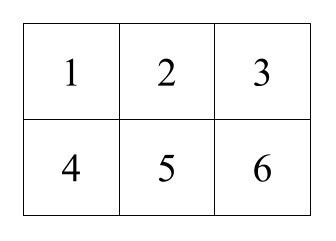
\includegraphics[width=0.25\textwidth]{figuras/posiciones.png}
\caption{Posibles posiciones de la ficha del segundo jugador en el juego ficha vs.\ dominó.}
\label{fig:posiciones}
\end{figure}

\begin{figure}[t]
\centering
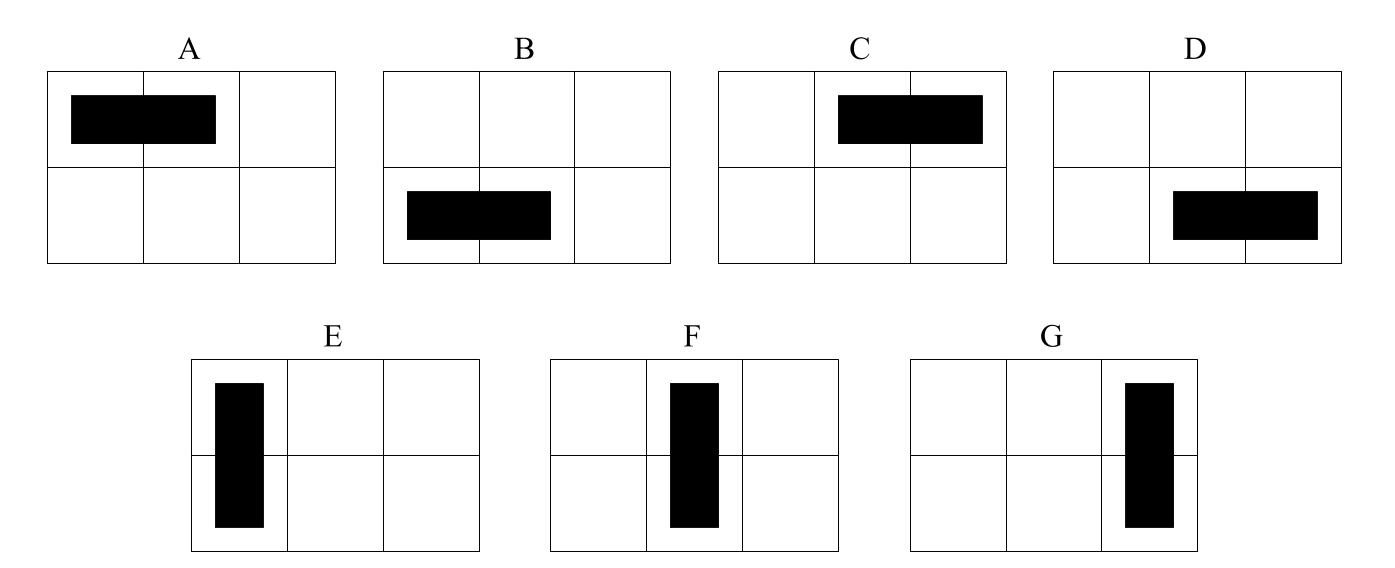
\includegraphics[width=\textwidth]{figuras/posiciones-domino.png}
\caption{Posibles posiciones de la ficha de dominó que representas las acciones del primer jugador en el juego ficha vs.\ dominó.}
\label{fig:posiciones-domino}
\end{figure}

\begin{table}[t]
\begin{center}
\caption{Matriz de pagos del juego ficha vs.\ dominó.}
\label{table:pagos-domino}
\begin{tabular}{ c | c | c | c | c | c | c |}
\multicolumn{1}{c}{}  &  \multicolumn{1}{c}{1} &  \multicolumn{1}{c}{2} & \multicolumn{1}{c}{3} & \multicolumn{1}{c}{4} & \multicolumn{1}{c}{5} & \multicolumn{1}{c}{6} \\ \cline{2-7}
A & -1 & -1 &  1 &  1 &  1 &  1 \\ \cline{2-7}
B &  1 &  1 &  1 & -1 & -1 &  1 \\ \cline{2-7}
C &  1 & -1 & -1 &  1 &  1 &  1 \\ \cline{2-7}
D &  1 &  1 &  1 &  1 & -1 & -1 \\ \cline{2-7}
E & -1 &  1 &  1 & -1 &  1 &  1 \\ \cline{2-7}
F &  1 & -1 &  1 &  1 & -1 &  1 \\ \cline{2-7}
G &  1 &  1 & -1 &  1 &  1 & -1 \\ \cline{2-7}
\end{tabular}
\end{center}
\end{table}

El problema de programación lineal asociado se encuentra en la Ecuación~\ref{apex:eq:pl-domino}. Este problema no tiene solución única (lo que implica que el juego no tiene un equilibrio de Nash único), una solución (primal y dual) viene dada por:

\begin{alignat}{1}
(z^*, x^*_1, x^*_2, x^*_4, x^*_5, x^*_6, x^*_6, x^*_7)\ =\ \left(\frac{1}{3}, \frac{1}{3}, \frac{1}{3}, 0, 0, 0, 0, \frac{1}{3}\right) \,, \\
(w^*, y^*_1, y^*_2, y^*_3,  y^*_4, y^*_5, y^*_6)\ =\ \left(\frac{1}{3}, \frac{1}{3}, 0, \frac{1}{3}, 0, \frac{1}{3}, 0\right) \,.
\end{alignat}

Esta solución corresponde a la estrategia en la que el jugador $1$ elige las posiciones A, B y G con probabilidad $\frac{1}{3}$ cada una, y el jugador $2$ elige las posiciones $1$, $3$, y $5$ con probabilidad $\frac{1}{3}$ cada una. Además, el valor del juego es igual a $\frac{1}{3}$. La Tabla~\ref{table:resultados-rm-domino} muestra el resumen de los resultados experimentales. Note que la máxima explotabilidad es igual a 0,01. Por otra parte, la Figura~\ref{fig:regret-rm-domino} muestra el \textit{regret} con respecto al número de iteraciones de este juego, donde se observa la convergencia del \textit{regret} en cada una de ellas.

\begin{table}[h]
\caption{Resultados Experimentales del juego ficha vs.\ dominó.}
\label{table:resultados-rm-domino}
\centering
\begin{tabular}{l r r r}
    \toprule
    & \multicolumn{1}{c}{A} & \multicolumn{1}{c}{B} & \multicolumn{1}{c}{C} \\ \midrule
    Ganancia esperada $u(\sigma)$ & 0,333 & 0,334 & 0,334  \\
    Explotabilidad $\varepsilon_{\sigma}$ & 0,010 & 0,007 & 0,004 \\
    Tiempo $T$ & 319,179 & 11,275 & 0,237  \\
    Iteraciones $I$ & 108.319.272,4 & 75.250,2 & 84.318,5 \\
    $T/I$ & $2,95 {\times} 10^{-6}$ & $1,50 {\times} 10^{-4}$ & $2,81 {\times} 10^{-6}$ \\
    \bottomrule
\end{tabular}
\end{table}
\graphicsRM{domino}{ficha vs.\ dominó}
 
\subsection*{Coronel Blotto}

En este juego cada uno de los jugadores tiene $S$ soldados en total que debe ubicar en $N$ campos de batallas. Cada soldado debe ser asignado a un único campo, pero cualquier número de soldados puede ser colocado en cualquier campo, incluyendo cero. Un jugador obtiene un campo de batalla si asigna más soldados que su oponente en ese campo de batalla. El juego es ganado por el jugador que obtenga un mayor número de campos y su pago es igual a la diferencia entre el número de campos obtenidos por cada uno de los jugadores \cite{bib:blotto-game}.

Formalmente el juego puede ser descrito de la siguiente manera. Cada jugador debe elegir $N$ números enteros, digamos $(a_1, a_2, ..., a_N)$ y $(b_1, b_2, ..., b_N)$, para el jugador $1$ y $2$ respectivamente, tales que $a_1 + a_2 + ... + a_N = S$ y $b_1 + b_2 + ... + b_N = S$, con $N < S$, donde $a_i$ y $b_i$ es la cantidad de soldados ubicados el $i$-ésimo campo por el primer y segundo jugador, respectivamente. La ganancia del jugador $1$ viene dada por:
\begin{alignat}{1}
|\{ 1 \leq i \leq N : a_i > b_i\}| - |\{ 1 \leq i \leq N : a_i < b_i\}| \,.
\end{alignat}

Este juego depende de dos parámetros: el número de soldados $S$ y el número de campos de batallas $N$, por lo que la matriz de pagos no es constante y por eso no es presentada como en los juegos anteriores. La matriz para un juego con $S$ soldados y $N$ es una matriz cuadrada de tamaño $\binom{N+S-1}{S-1}$.

En este juego es necesario generar la matriz de pagos dependiendo de los parámetros. Para esto se creó un programa que dado el número de campos de batalla ($N$) y el número de soldados ($S$), se generan todas las posibles distribuciones de cada uno de los jugadores mediante un algoritmo de \textit{backtracking}, y calcula el pago para cada juego posible, obteniendo como salida del programa la matriz deseada. De esta forma se generó la matriz de pagos para este juego cuando $N = 3$ y $S = 5$.

En este juego no se conoce un equilibrio de Nash teóricamente, para valores arbitrarios de $N$ y $S$. Sin embargo, debido a que la matriz de pagos es simétrica, el valor del juego debe ser igual a $0$. La Tabla~\ref{table:resultados-rm-blotto} muestra los resultados experimentales y la Figura~\ref{fig:regret-rm-coronel-blotto} muestra las gráficas del \textit{regret} con respecto al número de iteraciones para cada uno de los procedimientos; note la convergencia en cada uno de los casos.

\begin{table}[t]
\caption{Resultados Experimentales del juego coronel Blotto.}
\label{table:resultados-rm-blotto}
\centering
\begin{tabular}{l r r r}
    \toprule
    & \multicolumn{1}{c}{A} & \multicolumn{1}{c}{B} & \multicolumn{1}{c}{C} \\ \midrule
    Ganancia esperada $u(\sigma)$ & 0,000219 & 0,000150 & 0,000024 \\
    Explotabilidad $\varepsilon_{\sigma}$ & 0,010 & 0,010 & 0,009  \\
    Tiempo $T$ &  875,533 &  70,453 & 0,166 \\
    Iteraciones $I$ &  190.222.305,3 & 58.794,4  & 48.613,5 \\
    $T/I$ & $4,60{\times}10^{-6}$ & $1,20{\times}10^{-3}$ & $3,41{\times}10^{-6}$\\
    \bottomrule
\end{tabular}
\end{table}

\graphicsRM{coronel-blotto}{Coronel Blotto}
 
\section{Análisis de Experimentos}
A continuación, se analiza el desempeño de los procedimientos, comparándolos entre sí, observando la rapidez de convergencia de cada uno de ellos.

\subsection{Complejidad de Cada Iteración}

Los procedimientos cambian en la forma en que se elige la siguiente estrategia en cada iteración. En los procedimientos A y B se utiliza un regret condicional, en el que se mide el \textit{arrepentimiento} de cambiar una estrategia por otra. Esta métrica se debe mantener a lo largo de todas las iteraciones, por lo que cada iteración necesita memoria adicional de complejidad $\mathcal{O}(N^2 + M^2)$, donde $N$ y $M$ es el número de acciones posibles para el jugador $1$ y $2$, respectivamente. En el procedimiento C se utiliza únicamente el regret incondicional, por lo que la cantidad de memoria adicional es del orden $\mathcal{O}(N + M)$.

Con respecto a la complejidad de tiempo se tiene que los procedimientos de regret condicional e incondicional (A y C) son lineales en el número de acciones. Sin embargo, en el procedimiento B es necesario resolver un sistema de ecuaciones lineales para elegir cada estrategia nueva, del tamaño del número de acciones del jugador respectivo, obteniendo que la complejidad total es $\mathcal{O}(N^3 + M^3)$. La Tabla \ref{tab:complejidades-iteraciones} muestra un resumen de la complejidad en tiempo y memoria adicional.

\begin{table}[h]
    \caption{Complejidad por iteración de cada uno de los procedimientos.}
    \label{tab:complejidades-iteraciones}
    \centering
    \begin{tabular}{c c c}
        \toprule
         Procedimiento & Memoria & Tiempo  \\ \midrule
         A & $\mathcal{O}(N^2 + M^2)$ & $\mathcal{O}(N + M)$ \\ 
         B & $\mathcal{O}(N^2 + M^2)$ & $\mathcal{O}(N^3 + M^3)$ \\
         C & $\mathcal{O}(N + M)$     & $\mathcal{O}(N + M)$ \\ \bottomrule
    \end{tabular}
\end{table}

Por lo anterior, se observa que la velocidad de las iteraciones del procedimiento que calcula el vector invariante de probabilidad es más lenta en todos los casos, estando uno o dos órdenes de magnitud por encima, según el tamaño de la matriz. Por lo que, si la matriz es sumamente grande, el segundo método sería el menos adecuado.

\subsection{Número de Iteraciones}

Con respecto al número de iteraciones se nota, observando las Tablas~\ref{table:resultados-rm-matching-pennies}, \ref{table:resultados-rm-RPS}, \ref{table:resultados-rm-domino} y \ref{table:resultados-rm-blotto}, que el procedimiento A, \textit{regret} incondicional es el que necesita muchas más iteraciones para converger. Por otra parte, en algunos casos esta métrica fue menor en el procedimiento B y en otros casos el mínimo se obtuvo con el procedimiento C. También es importante destacar que en el juego de piedra, papel o tijera se tienen varios casos donde se obtiene la convergencia en menos de $10$ iteraciones (ver Apéndice \ref{apex:chapter:experimentos-rm}); esos son casos donde se obtiene el equilibrio de Nash de forma exacta en pocas iteraciones.

\subsection{Tiempo Transcurrido}

Observando el tiempo promedio de los procedimientos en las Tablas~\ref{table:resultados-rm-matching-pennies}, \ref{table:resultados-rm-RPS}, \ref{table:resultados-rm-domino} y \ref{table:resultados-rm-blotto}, se nota que el procedimiento A es el que emplea más tiempo en todos los casos, esto ocurre porque necesita muchas más iteraciones que los otros dos procedimientos. Por otra parte el procedimiento C es también más rápido que el procedimiento B, ya que la complejidad en cada iteración para resolver el sistema de ecuaciones ralentiza el tiempo total necesario, incluso, si la matriz es muy grande este procedimiento podría ser más lento que el procedimiento A y no sería factible.

Aunque el procedimiento donde se aplica \textit{Regret Matching} al regret incondicional (procedimiento C) es el más sencillo de implementar y el más rápido en converger, este procedimiento tiene una desventaja con respecto a los otros dos. Al utilizar el regret condicional, los dos primeros procedimientos garantizan que el regret condicional tiende a cero para cualquier par de estrategias de cada jugador y por lo tanto, conducen siempre a un equilibrio correlacionado. El tercer procedimiento sólo minimiza el regret incondicional y por lo tanto, si el juego es de más de dos jugadores o no es de suma cero, entonces ya no se puede garantizar que se encontrará alguna solución al juego.

\chapter{Counterfactual Regret Minimization}
\label{chapter:cfr}

El objetivo de este capítulo es presentar un algoritmo que permita encontrar un equilibrio de Nash en juegos en forma extensiva no determinista con información incompleta y probarlo empíricamente en distintos juegos. Aunque todo juego en forma extensiva puede ser representado en forma normal, esto no es de mucho interés pues la forma normal puede tener un tamaño exponencialmente más grande al tamaño del árbol. Se verá como el concepto de minimización del \textit{regret} puede ser extendido a juegos secuenciales, sin necesidad de la forma normal explícita. Los conceptos, procedimientos y teoremas mostrados en esta sección, son presentados en \cite{bib:cfr}.

\section{Descomposición del Regret}

La primera definición clave es la de \textit{regret}. Para esto, es necesario considerar jugar repetidamente un juego en forma extensiva. Sea $\sigma_i^t$ la estrategia usada por el jugador $i$ a tiempo $t$. La Definición \ref{def:average-overall-regret}, presenta el concepto de \textit{regret} promedio general.

\begin{definition}
\label{def:average-overall-regret}
El \textbf{regret promedio general} del jugador $i$ a tiempo $T$ es:
\begin{alignat}{1}
R_i^T\ =\ \max_{\sigma^* \in B_i} \, \frac{1}{T}\, \sum_{t = 1}^T \, u_i(\sigma_i^*, \sigma_{-i}^t) - u_i(\sigma^t) \,.
\end{alignat}
\end{definition}

\textcolor{red}{\bf **** Falta decir que es $\sigma_i^*$ y algun comentario de que mide $R^i_T$; e.g. el promedio de lo que el jugador $i$ dejor de ganar al no haber utilizado $\sigma_i^*$ ****}

Se denotará con $\bar{\sigma}_i^{T}$ la estrategia promedio, desde el tiempo 1 al tiempo $T$, del jugador $i$. En particular, para cada conjunto de información $I \in \mathcal{I}_i$ y para cada acción $a \in A(I)$ se define:
\begin{alignat}{1}
\bar{\sigma}_i^{T}(I)(a)\ =\ \frac{\sum_{t = 1}^T \pi^{\sigma^t_i}(I)\,\sigma^t_i(I)(a)}{\sum_{t = 1}^T \pi^{\sigma_i^t}(I)}
\end{alignat}
\textcolor{red}{\bf donde ... $\pi$ es .. y $\sigma$ es ...}

Esta estrategia es el promedio ponderado de las probabilidades $\sigma^t(I)(a)$ con respecto a que tan probable es alcanzar $I$ dado $\sigma_i^t$. La relación entre el \textit{regret} promedio general y el concepto de solución se muestra en el siguiente teorema.

\begin{theorem}
\label{theo:regret-nash}
En un juego de dos jugadores de suma cero si el regret promedio general a tiempo $T$ es menor que $\varepsilon$ entonces $\bar{\sigma}^{T}=(\bar\sigma^T_1,\bar\sigma^T_2)$ es un $2\varepsilon$-equilibrio de Nash.
\end{theorem}

Como consecuencia se obtiene que un algoritmo que lleve el \mbox{\textit{regret}} promedio general a cero conducirá a un equilibrio de Nash. La idea fundamental del enfoque presentado a continuación, propuesto en \cite{bib:cfr}, consiste en descomponer el \textit{regret} promedio general en un conjunto de términos aditivos de \textit{regret} que puedan ser minimizados de forma independientemente. En particular es necesario introducir un par de conceptos nuevos, la \textit{utilidad contrafactual} y el \textit{regret contrafactual inmediato}.

\begin{definition}
\label{def:utilidad-contrafactual}
Sea $\sigma$ un perfil estratégico e $I$ un conjunto de información (\textcolor{red}{\bf para el jugador $i$???}), la \textbf{utilidad contrafactual} del par $(\sigma,I)$ es la ganancia esperada dado que el conjunto $I$ es alcanzado y todos los jugadores juegan con la estrategia $\sigma$ con excepción del jugador $i$ que juega para alcanzar $I$. Formalmente, si $\pi^{\sigma}(h, h')$ denota la probabilidad  de ir de la historia $h$ a la historia $h'$ (ver abajo), entonces
\begin{alignat}{1}
u_i(\sigma, I)\ =\ \frac{\sum_{h \in I, z \in Z} \pi^{\sigma_{-i}}(h)\, \pi^{\sigma}(h, z)\, u_i(z)}{\pi^{\sigma_{-i}}(I)}
\end{alignat}
donde $\pi^{\sigma_{-i}}(I)$ denota ... y $Z$ denota el conjunto de nodos terminales en el árbol \textcolor{red}{\bf **** CHECK ****}
\end{definition}

La probabilidad $\pi^{\sigma}(h, h')$ de ir de la historia $h$ a la historia $h'$ usando el perfil $\sigma$ se define como \textcolor{red}{\bf **** CHECK ****}. \textcolor{red}{\bf **** También falta algun comentario que le de sentido a esta definición... en línea con el algoritmo de RM visto anteriormente... ****}

Para toda acción $a$ en $A(I)$, se define $\sigma|_{I \rightarrow a}$ como el perfil estratégico que es idéntico a $\sigma$ excepto que el jugador $i$ siempre elige $a$ en el conjunto de información $I$.

\begin{definition}
\label{def:regret-inmediato}
El \textbf{regret contrafactual inmediato} es:
\begin{alignat}{1}
R_{i, \text{imm}}^T(I)\ =\  \max_{a \in A(I)} \, \frac{1}{T} \, \sum_{t = 1}^T \, \pi^{\sigma_{-i}^t}(I) \biggl[ u_i(\sigma^t|_{I \rightarrow a}, I) - u_i(\sigma^t, I) \biggr]\,.
\end{alignat}
\end{definition}

Intuitivamente, el \textit{regret} contrafactual inmediato es el arrepentimiento del jugador $i$ en su decisión sobre el conjunto de información $I$, en términos de la utilidad contrafactual, con un término de ponderación adicional para la probabilidad contrafactual que $I$ alcanzaría en esa ronda si el jugador hubiera intentado hacer eso. Usualmente, es de mayor interés el \textit{regret} cuando es positivo, por lo que se define $R_{i, \text{imm}}^{T, +} (I) = \max\{R^T_{i, \text{imm}} (I), 0\}$. Luego, se tiene el siguiente resultado:

\begin{theorem}[\textcolor{red}{\bf **** REF ****}]
\begin{alignat}{1}
R_i^T\ \leq\ \sum_{I \in \mathcal{I}_i} R_{i, \text{imm}}^{T, +}(I) \,.
\end{alignat}
\end{theorem}

Debido a que minimizar el \textit{regret} contrafactual inmediato concuce a minimizar el \textit{regret} promedio general es posible enfocarse en minimizar los primeros para obtener un equilibrio de Nash.

\section{Regret Minimization}

Antes de mostrar el algoritmo principal, denominado \textit{Counterfactual Regret Minimization} (CFR) para los juegos en forma extensiva, es necesario introducir el algoritmo general de \textit{Regret Minimization}. Este algoritmo puede ser descrito en un dominio donde hay un conjunto fijo de acciones $A$, una función de utilidad $u^t : A \rightarrow \mathbb{R}$, y en cada ronda $t$ una distribución de probabilidad $p^t$ es elegida.

\begin{definition}
\label{def:regret}
El \textit{regret} promedio de no haber elegido la acción $a \in A$ hasta tiempo $T$, y en su lugar elegir la acción $a'$ con probabilidad $p^t(a')$ para $t=1,2,\ldots,T$, se define como:
\begin{alignat}{1}
R^T(a)\ =\ \frac{1}{T} \sum_{t = 1}^T \left[u^t(a) - \sum_{a' \in A}p^t(a')u^t(a')\right] \,.
\end{alignat}
\end{definition}

El algoritmo de \textit{Regret Minimization} consiste en utilizar una distribución de probabilidad $p^t$, a tiempo $t$, definida por
\begin{alignat}{1}
p^t(a)\ =\ 
\begin{cases}
\frac{R^{t, +}(a)}{\sum_{a' \in A} R^{t, +}(a')}\ & \text{si }\ \sum_{a' \in A} R^{t, +}(a') > 0 \,, \\
\frac{1}{|A|}\ & \text{en otro caso} \,.
\end{cases}
\end{alignat}
donde $R^{t, +}(a) = \max\{R^t(a), 0\}$. 


\begin{theorem}[\textcolor{red}{\bf **** REF ****}]
Si $|u| = \max_{t \in \{1, 2, ... T\}} \max_{a, a' \in A}\bigl[u^t(a) - u^t(a')\bigr]$, entonces el regret del algoritmo de Regret Minimization está acotado por:
\begin{alignat}{1}
\max_{a \in A}\,R^t(a)\ \leq\ |u| \sqrt{\frac{|A|}{T}} \,.
\end{alignat}
\end{theorem}

\section{Counterfactual Regret Minimization (CFR)}
\label{section:cfr}

El algoritmo de \textit{Counterfactual Regret Minimization} es una aplicación del algoritmo \textit{Regret Minimization} de forma independiente a cada conjunto de información. En particular, se mantiene para cada conjunto de información $I \in \mathcal{I}_i$ y cada acción $a \in A(I)$, la medida de regret:
\begin{alignat}{1}
R_i^T(I, a)\ =\ \frac{1}{T} \sum_{t = 1}^T \pi^{\sigma^t_{-i}}(I)\biggl[u_i(\sigma^t|_{I \rightarrow a}, I) - u_i(\sigma^t, I)\biggr]
\end{alignat}

Se definimos $R_i^{T, +}(I, a) = \max\{R_i^T(I, a), 0\}$, la estrategia $\sigma^{T+1}_i$ elegida por el jugador $i$ a tiempo $T+1$ es:
\begin{alignat}{1}
\label{eq:cfr-regret-matching}
\sigma_i^{T+1}(I)(a)\ =\
\begin{cases}
\frac{R_i^{T, +}(I, a)}{\sum_{a' \in A(I) R_i^{T, +}(I, a')}}\ & \text{si } \sum_{a' \in A(I) R_i^{T, +}(I, a')} > 0 \,, \\
\frac{1}{|A(I)|}\ & \text{en otro caso.} 
\end{cases}
\end{alignat}

Este algoritmo consiste en seleccionar las acciones de forma proporcional a la cantidad del \textit{regret} contrafactual positivo de no haber elegido esa acción. Si ninguna de estas cantidades es positiva, entonces la acción se elige con una distribución uniforme. Luego, como cota de convergencia, se tiene el siguiente resultado:

\begin{theorem}[\textcolor{red}{\bf **** REF ****}]
Si el jugador $i$ selecciona las acciones de acuerdo al procedimiento anterior, entonces $R^T_{i, \text{imm}}(I) \leq \Delta_{u, i} \sqrt{|A_i|/T}$ donde $\Delta_{u,i} = \textcolor{red}{\bf *****}$, y por lo tanto
\begin{alignat}{1}
R_i^T\ \leq\ \sum_{I\in\mathcal{I}_i} R^{T,+}_{i,imm}(I) \ 
        \leq\ \Delta_{u,i}\,|\mathcal{I}_i|\,\sqrt{\frac{|A_i|}{T}}
\end{alignat}
donde $|A_i| = \max \{ |A(h)| : P(h) = i \}$ es el máximo número de acciones que el jugador $i$ tiene disponibles en una historia dada.
\end{theorem}


\section{Monte Carlo Conterfactual Regret Minimization (MCCFR)}

En la versión presentada del algoritmo CFR es necesario recorrer el árbol completo en cada iteración, algo que puede ser muy ineficiente cuando el árbol es muy grande. Dicha versión se conoce como \textit{vanilla} CFR. En \cite{bib:montecarlo-cfr} se describe una familia general de algoritmos CFR (basados en muestreo) denominada Monte Carlo Conterfactual Regret Minimization (MCCRF) que evitan recorrer el árbol de forma completa en cada iteración.

La idea general es restringir los estados terminales alcanzados en cada iteración, pero manteniendo el mismo valor esperado para la utilidad contrafactual. Sea $\mathcal{Q} = \{Q_1, Q_2, ..., Q_r\}$ un conjunto de subconjuntos de $Z$ (el conjunto de nodos terminales en el àrbol) tal que su unión sea igual a $Z$. Cada uno de estos conjuntos será llamado un bloque. Sea $q_j > 0$ la probabilidad de considerar el bloque $Q_j$ en la iteración actual donde $\sum_{j = 1}^r {q_j} = 1$, y sea $q(z) = \sum_{j | j \in Q_i}$ \textcolor{red}{\bf **** CHECK ****} la probabilidad de considerar el nodo terminal $z$ para la iteración actual. La utilidad contrafactual muestreada, cuando se actualiza el bloque $j$ se define como
\begin{alignat}{1}
\tilde{u}_i(\sigma, I | j)\ =\ \sum_{h \in I, z \in Q_j} \frac{\pi^{\sigma_{-i}}(h)\,\pi^{\sigma}(h, z)\, u_i(z)}{q(z)\,\pi^{\sigma_{-i}}(I)} \,.
\end{alignat}

Lo interesante es que la esperanza de la utilidad contrafactual muestreada coincide con la utilidad contrafactura, como se muestra a continuación.

\begin{theorem}[\textcolor{red}{\bf **** REF ****}]
\label{theo:esperanza-MCCFR}
$E_{j \sim q_j} [\tilde{u}_i(\sigma, I | j)]\ =\ u_i(\sigma, I)$.
\end{theorem}

Si se elige un único bloque $Q_1=Z$, $\mathcal{Q} = \{Q_1\}$, que contiene todas las historias terminales y para el cual $q_1=1$, la utilidad contrafactual muestreada se convierte en la utilidad contrafactual, y se obtiene el algoritmo \textit{vanilla} CFR. Sin embargo, si se eligen los bloques para que incluyan todas las historias terminales con la misma secuencia de acciones en los nodos de azar \textcolor{red}{\bf **** ??? ****} se obtiene un algoritmo que se denomina \textit{chance-sampled} CFR, siendo este último la versión utilizada para estudiar los juegos presentados en este trabajo de grado. El algoritmo se implemento como es detallado en \cite{bib:introductionCFR} y que se presenta en el Apéndice~\ref{apex:chapter:algoritmos}.


\section{Detalles de Implementación y Ejecución}

Los algoritmos y la representación de los juegos fueron implementados en el lenguaje C++ utilizando la librería estándar y una librería adicional llamada \textit{Boost} \cite{bib:boost} para obtener funciones de hash de los diferentes tipos de datos utlizados. Para la representación de los juegos se utilizó una clase abstracta llamada \functionname{Game}, que recibe como \textit{template} los tipos para el estado, las acciones, las propiedades, los conjunto de información, y la función de hash del juego específico.

Esta clase contiene las funciones virtuales necesarias para recorrer el árbol del juego de forma \textbf{implícita}, tales como: \functionname{actions}, que retornan las acciones del juego en el estado actual, \functionname{update\_state}, que actualiza el estado del juego dada una acción a realizar, \functionname{terminal\_state} que indica si un estado es terminal o no, \functionname{utility} que retorna la utilidad en un estado terminal, entre otras. Los algoritmos CFR y GEBR utilizan esta clase abstracta en su implementación. \textcolor{red}{\bf **** GEBR? ****}

Para cada tipo de juego, se creó una clase derivada de la clase \functionname{Game} en donde se especializan las funciones virtuales de la clase \functionname{Game} según las reglas de cada juego. De esta forma se puede utilizar la misma implementación de los algoritmos para todos los juegos.

Cabe destacar que todos los juegos fueron representados mediantes árboles con la raíz como único nodo de azar. Algunos juegos tienen esta representación de forma natural, por ejemplo, el Kuhn Poker, ya que las cartas se reparten al inicio y luego se juega acorde a esa distribución, sin volver a introducir ninguna jugada aleatoria. Otros juegos pueden tener nodos de azar distintos a la raíz; sin embargo, siempre es posible transformarlos a un árbol que represente el mismo juego donde todos los nodos de azar son condensados en la raíz y cada hijo de la raíz representa una elección por cada uno de los nodos de azar del árbol original. En esta representación se asume que todas las decisiones aleatorias se toman al inicio del juego.

La clase \functionname{Game} y todos los algoritmos son implementados suponiendo a la raíz como único nodo de azar en el juego. Además, se omiten los conjuntos de información donde existe una única acción posible, ya que en estos casos no hay ninguna decisión que tomar. 

Las ejecuciones de los algoritmos se realizaron en \textit{Amazon Web Services} (AWS), utilizando el servicio \textit{Amazon Elastic Compute Cloud} (Amazon EC2), instanciando máquinas virtuales con las siguientes caracteríscas:
\begin{itemize}[noitemsep]
    \item Procesador: Intel Broadwell E5-2686v4 \makeatletter{@} 2.3GHz.
    \item 8 cores y 32Gb de memoria RAM.
    %\item Sistema Operativo: Amazon Linux 2 AMI (HVM).
\end{itemize}

Para probar los algoritmos se implementaron tres clases de juegos diferentes: \textit{One Card Poker} (OCP), \textit{Dudo}, un juego de dados, y una versión del juego de dominó para $2$ personas. Se crearon varias instancias por clase de acuerdo a los parámetros de inicialización que reciben cada uno de ellas. Para la resolución de cada instancia se utilizó el algoritmo de CFR \textcolor{red}{\bf *** CUAL VERSION? ***} y se iteró sobre el árbol durante $10$ horas aproximadamente. Una vez terminado el tiempo asignado se calculó la mejor respuesta para cada jugador y la explotabilidad. 

En este trabajo, consideramos que una instancia de un juego se considera resuelta si la explotabilidad de la estrategia obtenida es menor que el $1\%$ de la mínima unidad de utilidad posible en el juego.

Para evaluar la convergencia de los algoritmos y la estrategia obtenida se utilizaron las métricas de \textit{regret} y explotabilidad, respectivamente. Para calcular la explotabilidad en estos juegos se implementó el algoritmo propuesto en \cite{bib:thesis-marc-lanctot}, denominado \textit{Generalized Expectimax Best Response} (GEBR), descrito en el Apéndice~\ref{apex:chapter:algoritmos}. La complejidad de este algoritmo es $\mathcal{O}(ND)$ donde $N$ es el número de nodos del árbol y $D$ es la profundidad del árbol. Note que el algoritmo tiene una alta complejidad por lo que se usa únicamente para calcular la explotabilidad de la estrategia final.

Por cada juego se presenta una tabla que resume los resultados. Estas tablas contienen el número de nodos del árbol ($N$), el número de conjuntos de información ($I$), el valor del juego usando la estrategia obtenida ($u({\sigma})$), y la explotabilidad ($\varepsilon_{\sigma}$) calculada por GEBR. Se agrega además, en cada tabla, el número de iteraciones realizadas durante el tiempo de entrenamiento y la última columna indica si el juego fue resuelto o no, según lo establecido anteriormente. Por último, también se muestra la gráfica del \textit{regret} con respecto al número de iteraciones sobre algunas de las instancias de cada juego. Las gráficas completas pueden ser encontradas en el Apéndice~\ref{apex:chapter:experimentos-cfr}.

\subsection*{One-Card Poker}
\textit{One-Card Poker}, abreviado OCP($N$), es la versión generalizada del juego Kuhn Póker, explicado en el Capítulo \ref{section:kuhn-poker}. En este juego, cada jugador recibe una carta de un mazo de $N$ cartas y luego pueden apostar o retirarse según las mismas reglas del Kuhn Poker. Note que OCP(3) es equivalente al Kuhn Poker. El árbol de este juego tiene $9N(N-1)+1$ nodos (incluyendo el nodo inicial, que es el nodo de azar) y hay $4N$ conjuntos de información entre ambos jugadores. 

La Tabla \ref{table:resultados-CFR-OCP} muestra un resumen de los resultados de las instancias del juego OCP. Se observa que se lograron resolver todas los casos propuestos. La Gráfica~\ref{fig:cfr-regret-ocp-200} muestra el \textit{regret} con respecto al número de iteraciones en el juego OCP$(200)$. Se observa que al principio el regret aumenta debido a que el regret se inicializa en $0$ y empieza a aumentar a medida que se descubren los conjuntos de información. Luego, se observa como converge a $0$ a medida que transcurren las iteraciones.

\begin{table}[h]
    \centering
    \caption{Resultados del algoritmo CFR en el juego OCP($N$) con diferentes números de cartas $N$.}
    \label{table:resultados-CFR-OCP}
    \begin{tabular}{lrrrrrc}
        \toprule
        Juego & $N$ & $I$ & Iteraciones & $u(\sigma)$ & $\varepsilon_{\sigma}$ (\%) & Resuelto \\ \midrule
        OCP$(3)$        &          55 &      12 & 1.181.763.638 & -0,056 & 0,0098 & \cmark \\
        OCP$(12)$       &       1.189 &      48 & 1.147.919.240 & -0,062 & 0,0032 & \cmark \\
        OCP$(50)$       &      22.051 &     200 & 1.145.291.974 & -0,058 & 0,0099 & \cmark \\
        OCP$(200)$      &     358.201 &     800 & 1.128.993.847 & -0,056 & 0,0078 & \cmark \\
        OCP$(1000)$     &   8.991.001 &   4.000 & 1.087.573.694 & -0,056 & 0,0098 & \cmark \\
        OCP$(5000)$     & 224.955.001 &  20.000 & 1.038.367.354 & -0,056 & 0,0241 & \cmark \\
        \bottomrule
    \end{tabular}
\end{table}

\begin{figure}[h]
    \centering
    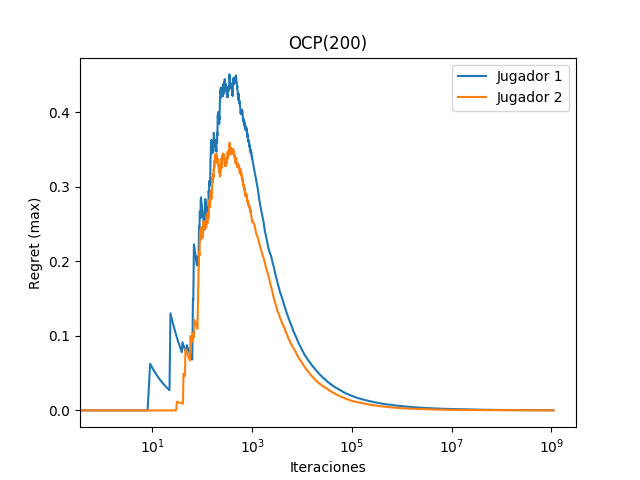
\includegraphics[width=0.5\textwidth]{graficas/cfr/ocp/OCP(200).png}
    \caption{Gráficas del \textit{regret} con respecto al número de iteraciones del juego \textit{One Card Poker} $(200)$. \textcolor{red}{**** poner otra gráfica, 2 gráficas horizontales por juego ****}}
    \label{fig:cfr-regret-ocp-200}
\end{figure}

\subsection*{Dudo}
Dudo, también conocido como \textit{Bluff}, \textit{Liar's Dice} o Perudo, es un juego de dados y apuestas. Usualmente se juega entre $2$ y $6$ jugadores. Los jugadores se ubican en forma circular y cada uno de ellos tiene un número de dados. De forma simultánea, todos lanzan sus dados, cada jugador puede ver el resultado de sus propios dados, pero no puede ver el resultado de los dados de los otros jugadores. Una vez hecho esto, los jugadores empiezan a apostar sobre el número de veces que apareció una cara en específico en todos los dados que hay en la mesa.

Una apuesta consiste en decir $2$ números $(x, y)$. Esto indica que el jugador apuesta que hay al menos $x$ dados cuyo resultado fue el número $y$. El primer jugador (que se elige previamente mediante el lanzamiento de 1 dado o de alguna otra forma), realiza la primera apuesta y, en sentido horario, cada jugador puede hacer una apuesta más alta o decir \say{dudo} y retar al jugador anterior. Una apuesta es más alta que otra si el número de dados que se anuncian en la apuesta ($x$) es mayor, o si el número de dados es igual, pero la cara apostada ($y$) es mayor. Por ejemplo $(3, 1)$ es mayor que $(2, 5)$, y ambas apuestas son mayores que $(2, 3)$.

Por otra parte, si un jugador reta al jugador previo, se descubren todos los dados de todos los jugadores. Si la cantidad de dados con la cara $y$ es mayor o igual a $x$, donde $(x, y)$ fue la apuesta realizada por el jugador, el jugador que hizo el reto pierde un dado. En caso contrario, el jugador que hizo la apuesta pierde un dado. Luego, todos los jugadores lanzan sus dados nuevamente y una nueva ronda de apuestas empieza por el jugador que perdió la ronda anterior. Un jugador pierde cuando se queda sin dados, el ganador es el último jugador con al menos un dado restante. La figura \ref{fig:dudo} muestra una foto del juego de \textit{Perudo}, una versión comercial de este juego, que está diseñada para $6$ jugadores, donde cada jugador empieza con $5$ dados. En la figura se observan los vasos que se utilizan para lanzar los dados y evitar que cada jugador vea los dados de los demás.

\begin{figure}[t]
    \centering
    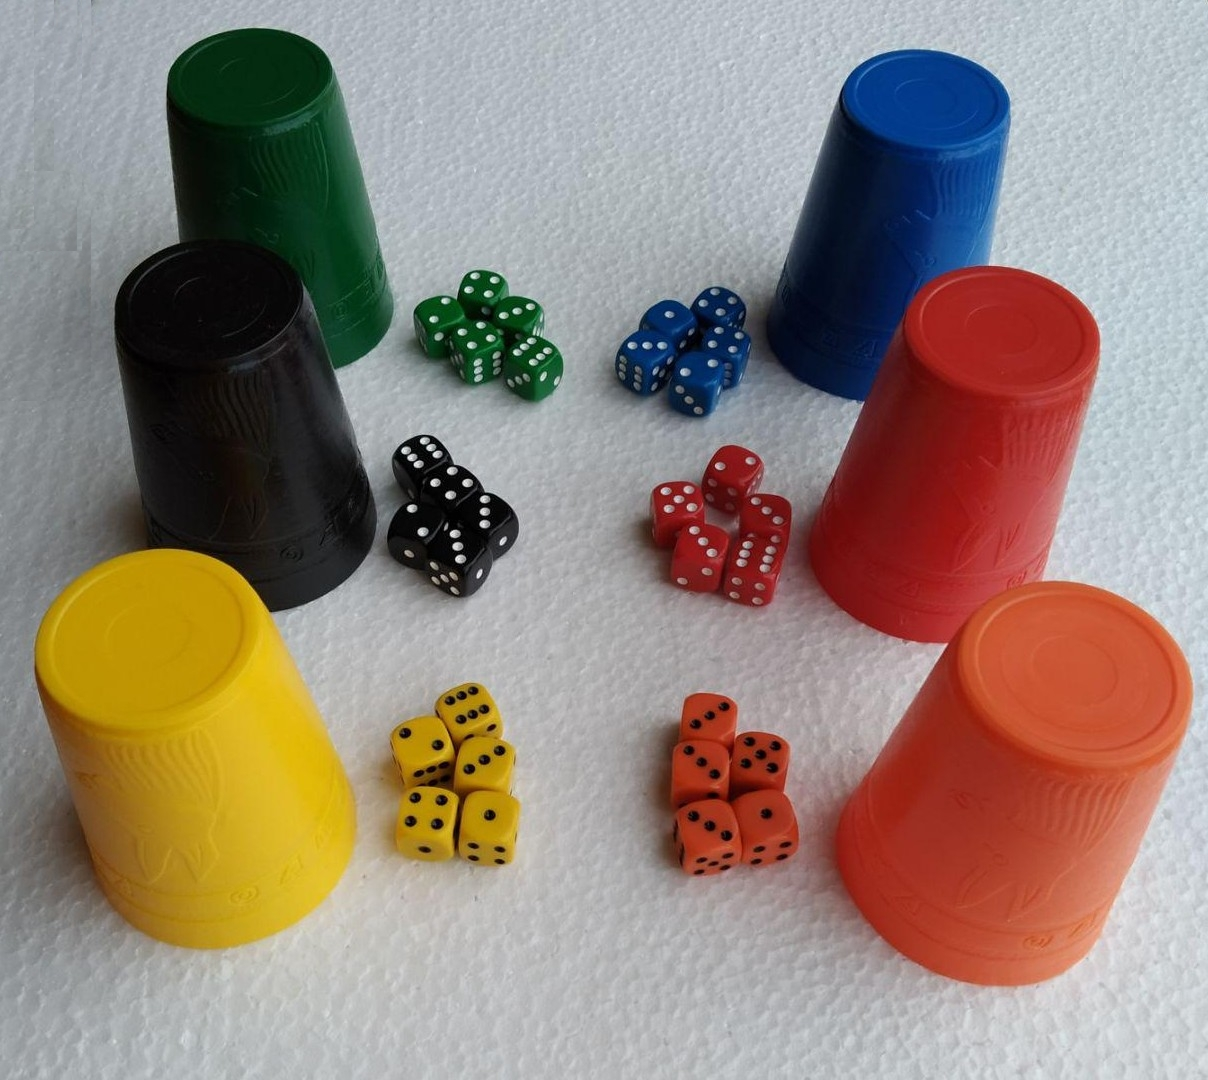
\includegraphics[width=0.4\textwidth]{figuras/dudo.jpg}
    \caption{Juego dudo. Los vasos se utilizan para lanzar los dados y evitar que los oponentes vean el resultado.}
    \label{fig:dudo}
\end{figure}

En este trabajo consideraremos este juego para $2$ jugadores únicamente. Dudo$(K, D_1, D_2)$ hará referencia a una única ronda de apuestas de $2$ jugadores, donde el primer jugador tiene $D_1$ dados, el segundo jugador tiene $D_2$ dados y cada dado tiene $K$ caras. El juego completo consiste en múltiples rondas, donde $D_1$ o $D_2$ disminuye en una unidad al finalizar cada ronda. Cuando uno de los jugadores pierde todos los dados obtiene una utilidad de $-1$, mientras que su oponente obtiene una utilidad de $1$. En este juego cada ronda se considerará un subjuego y se representará con un árbol independiente, donde los valores esperados para los juegos Dudo$(K, D_1 - 1, D_2)$ y Dudo$(K, D_1, D_2 - 1)$ se precalculan y se utilizan como utilidad para las hojas del árbol Dudo$(K, D_1, D_2)$. Note que en el juego estándar $K$ siempre tiene un valor de $6$.

Cuando el jugador $i$ lanza $D_i$ dados hay $\binom{D_i+K-1}{K-1}$ resultados diferentes posibles, ya que cada resultado puede ser representado con una tupla $(a_1, a_2, ..., a_k)$, donde $a_j$ representa el número de dados con la cara $j$, por lo que $\sum_j^K = D_i$ y $a_j \geq 0$. Por otra parte, cada secuencia de apuestas puede ser representada por una secuencia binaria de longitud $K(D_1 + D_2)$ donde el $i$-ésimo bit es $1$ si la $i$-ésima secuencia más alta fue dicha durante la ronda, y $0$ en caso contrario. Por ejemplo, si $D_1 = D_2 = 1$, las apuestas $(1, 1)-(1, 3)-(1, 6)-(2, 4)-(2, 5)-(1, 6)$ se representa con la secuencia binaria $101001000110$. Por lo tanto, existen $2^{K(D_1 + D_2)}$ secuencias diferentes. Cada secuencia pertenece a un jugador en específico, por lo que si $D_1 = D_2$, el número de conjuntos de información es igual a  $\binom{D_i+K-1}{K-1}2^{K(D_1 + D_2)}$, incluyendo los conjuntos de información con una única acción posible. Para excluir estos conjuntos de información, debemos excluir las secuencias donde la última apuesta es la máxima apuesta posible, pues el siguiente jugador sólo podría decir \say{dudo}. La cantidad de estas secuencias es igual a $2^{K(D_1 + D_2)-1}$. Luego, el número de conjuntos de información con más de una acción posible es igual a $\binom{D_i+K-1}{K-1}2^{K(D_1 + D_2)-1}$ dado que ambos jugadores tienen el mismo número de dados.

Para contar el número total de nodos, se puede considerar el lanzamiento de los dados de forma independiente, pues las secuencias posibles de apuestas no dependen del resultado de los dados. Por lo expuesto anteriormente, el número posible de apuestas es igual a $2^{K(D_1+D_2)}$, pero después de cada secuencia siempre se puede decir \say{dudo}, salvo para la secuencia vacía. El número total de nodos (incluyendo nodos terminales y no terminales) es igual a $\binom{D_1+K-1}{K-1}\binom{D_1+K-1}{K-1}(2^{K(D_1+D_2)+1}-1)+1$.

La Tabla~\ref{table:resultados-CFR-dudo} muestra el resumen de los resultados de las instancias del juego dudo. En este juego no se alcanzó la cota deseada para la explotabilidad para las instancias Dudo$(4, 2, 2)$, Dudo$(5, 2, 2)$, Dudo$(6, 1, 2)$ y Dudo$(6, 2, 1)$, siendo la instancia Dudo$(5, 2, 2)$ la que posee la estrategia más explotable con más del $15\%$ de la ganancia posible. Esto debido al bajo número de iteraciones realizadas durante el entrenamiento (menos de $4.000$) por el gran tamaño del árbol. La Gráfica~\ref{fig:cfr-regret-dudo-5-2-2} corresponde al juego Domino$(5, 2, 2)$. Esta tiene un comportamiento similar a la gráfica anterior pero se observa que la convergencia está inconclusa, por lo que la estrategia final encontrada para Dudo$(5, 2, 2)$ tiene alta explotabilidad.

\begin{table}[h]
    \centering
    \caption{Resultados del algoritmo CFR en el juego dudo.}
    \label{table:resultados-CFR-dudo}
    \begin{tabular}{lrrrrrc}
        \toprule
        Juego & $N$ & $I$ & Iteraciones & $u(\sigma)$ & $\varepsilon_{\sigma}$ (\%) & Resuelto \\ \midrule
        Dudo$(3, 1, 1)$ &         1.144 &          96 & 77.243.464 & -0,111 &  0,0098 & \cmark \\
        Dudo$(3, 1, 2)$ &        18.415 &       1.152 & 10.050.143 & -0,465 &  0,0211 & \cmark \\
        Dudo$(3, 2, 1)$ &        18.415 &       1.152 &  9.903.467 &  0,506 &  0,0111 & \cmark \\
        Dudo$(3, 2, 2)$ &       294.877 &      12.288 &  1.137.993 & 0,0054 &  0,2887 & \cmark \\
        Dudo$(4, 1, 1)$ &         8.177 &         512 & 18.697.532 & -0,125 &  0,0259 & \cmark \\
        Dudo$(4, 1, 2)$ &       327.641 &      14.366 &  1.215.600 & -0,508 &  0,0971 & \cmark \\
        Dudo$(4, 2, 1)$ &       327.641 &      14.366 &  1.213.799 &  0,552 &  0,3701 & \cmark \\
        Dudo$(4, 2, 2)$ &    13.107.101 &     327.680 &     63.109 & 0,0069 &  2,1132 & \xmark \\
        Dudo$(5, 1, 1)$ &        51.176 &       2.560 &  4.521.208 & -0,120 &  0,1186 & \cmark \\
        Dudo$(5, 1, 2)$ &     4.915.126 &     163.840 &    151.235 & -0,565 &  0,6197 & \cmark \\
        Dudo$(5, 2, 1)$ &     4.915.126 &     163.840 &    143.698 &  0,581 &  0,0122 & \cmark \\
        Dudo$(5, 2, 2)$ &   471.858.976 &   7.864.320 &      3.826 &  0,836 & 15,1963 & \xmark \\
        Dudo$(6, 1, 1)$ &       294.877 &      12.288 &  1.067.782 & -0,111 &  0,0975 & \cmark \\
        Dudo$(6, 1, 2)$ &    66.060.163 &   1.769.472 &     17.702 & -0,593 &  4,5781 & \xmark \\
        Dudo$(6, 2, 1)$ &    66.060.163 &   1.769.472 &     17.221 &  0,592 &  3,9594 & \xmark \\
        \bottomrule
    \end{tabular}
\end{table}

\begin{figure}[h]
    \centering
    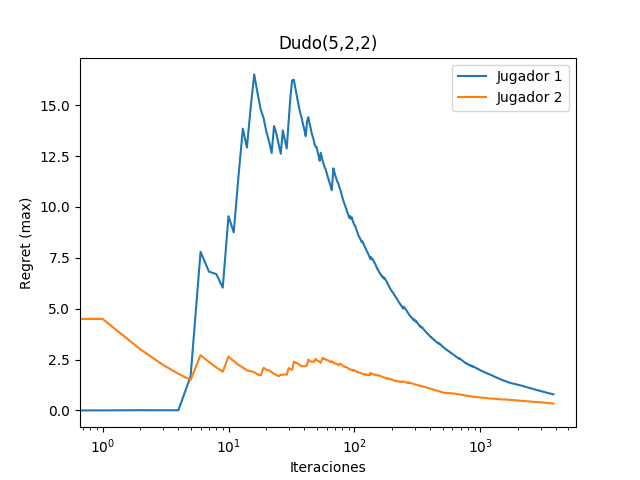
\includegraphics[width=0.5\textwidth]{graficas/cfr/dudo/Dudo(5,2,2).png}
    \caption{Gráficas del \textit{regret} con respecto al número de iteraciones del juego Dudo $(5, 2, 2)$.}
    \label{fig:cfr-regret-dudo-5-2-2}
\end{figure}

\subsection*{Dominó para Dos Jugadores}
%En este trabajo se utilizó una versión de este juego para $2$ jugadores. 
Al inicio del juego cada jugador toma una cantidad específica de piezas de forma aleatoria y las piezas restantes se dejan sin descubrir para ser usadas en turnos posteriores. Al igual que en el juego tradicional de dominó, los jugadores juegan por turnos alternados (el primero jugador se elige de forma arbitraria). Cada uno debe colocar una ficha válida acorde a las reglas \textit{estándares} en Venezuela del juego. Si un jugador no puede colocar una ficha toma una ficha de las que no están descubiertas (si todavía hay disponibles), el jugador verifica si puede colocar la ficha tomada y en caso contrario pasa el turno y juega el oponente.
El juego termina cuando alguno de los jugadores usa todas las piezas o cuando ambos jugadores no pueden jugar ni tomar piezas nuevas; en este último caso se dice que el juego está bloqueado. El ganador es el jugador que se queda sin piezas o, en caso de bloqueo, el jugador que acumule menos puntos en todas las piezas que quedaron en su mano. La utilidad obtenida es el número de puntos que el jugador perdedor acumuló en las piezas que quedaron en su mano (con signo positivo para el jugador ganador y signo negativo para el perdedor). Cabe destacar que sólo se puede tomar una pieza o pasar, si no se puede realizar una jugada con la mano actual.

Usualmente se utilizan $28$ piezas, donde las piezas pueden tener entre $0$ y $6$ puntos en cada extremo, y cada jugador recibe $7$ piezas al inicio del juego. En este trabajo se parametriza el número máximo de puntos que puede tener una ficha, así como la cantidad de piezas repartidas inicialmente. De esta forma Domino$(M, N)$ refiere a un juego donde las piezas tienen entre $0$ y $M$ puntos (con un total de $(M+1)(M+2)/2$ piezas) y cada jugador recibe $N$ piezas al inicio del juego.

En este juego no es fácil calcular el tamaño del árbol y el número de conjuntos de información, principalmente porque las acciones posibles en un estado dependen tanto de la mano del jugador como de las piezas en la mesa. En el Kuhn Poker siempre hay $2$ acciones posibles (${pasar, apostar}$) y en el Dudo las acciones disponibles dependen únicamente de la última apuesta y no dependen de los dados que tengan los jugadores. Así que estos parámetros fueron determinados recorriendo el árbol del juego mediante búsqueda en profundidad.

La Tabla~\ref{table:resultados-CFR-domino} muestra el resumen de los resultados del juego dominó. En este caso no fue posible resolver la instancia Domino$(3, 4)$ con respecto a los juegos de dominó. La Gráfica~\ref{fig:cfr-regret-domino-3-3} muestra el \textit{regret} con respecto al número de iteraciones del juego Domino$(3, 3)$. Al igual que en las gráficas anteriores, se observa como el regret crece al principio para luego converger a $0$.

\begin{table}[h]
    \centering
    \caption{Resultados del algoritmo CFR en el juego dominó.}
    \label{table:resultados-CFR-domino}
    \begin{tabular}{lrrrrrc}
        \toprule
        Juego & $N$ & $I$ & Iteraciones & $u(\sigma)$ & $\varepsilon_{\sigma}$ (\%) & Resuelto \\ \midrule
        Domino$(2, 2)$ &         7.321 &     102 & 585.191.577 & 2,4000 & 0,0000 & \cmark \\
        Domino$(3, 2)$ &    46.534.657 &  88.947 & 436.905.363 & 2,8767 & 0,0292 & \cmark \\
        Domino$(3, 3)$ &   246.760.993 & 107.854 &  79.751.183 & 2,1539 & 0,3599 & \cmark \\
        Domino$(3, 4)$ & 1.547.645.185 & 104.050 &  11.984.261 & 3,2034 & 1,3630 & \xmark \\
        \bottomrule
    \end{tabular}
\end{table}

\begin{figure}[h]
    \centering
    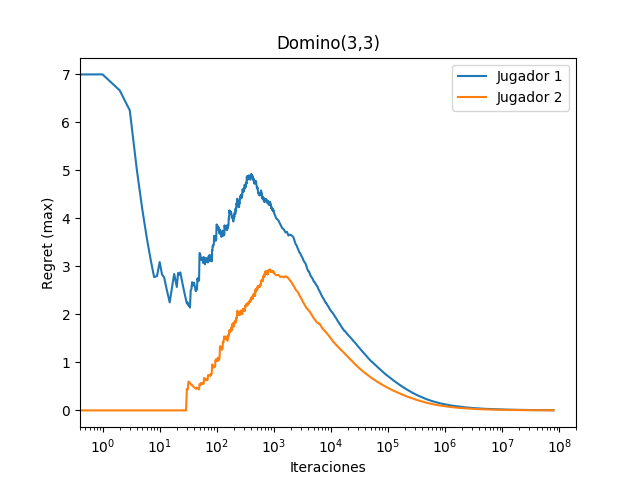
\includegraphics[width=0.5\textwidth]{graficas/cfr/domino/Domino(3,3).png}
    \caption{Gráficas del \textit{regret} con respecto al número de iteraciones del juego Dominó $(3, 3)$.}
    \label{fig:cfr-regret-domino-3-3}
\end{figure}


\chapter*{Conclusiones}

Sugerencias y revisiones de esta clase enviarlos a los correos \texttt{ccontreras@usb.ve} y \texttt{asajo@usb.ve}.
\nocite{*}
\bibliography{epilogo/referencias}
\appendix
\chapter{Resultados Experimentales, Regret Matching en Juegos en Forma Normal}

En este apéndice se presentan las tablas y gráficas detalladas para los juegos en forma normal descritos en la sección \ref{section:descripcion-juegos-fn}. Para cada juego se muestra una tabla con la estrategia obtenida en la última corrida de cada uno de los procedimientos y, en caso de conocerse, el equilibrio de Nash. Para cada estrategia se muestra la utilidad de cada jugador si utilizan una mejor respuesta frente a la estrategia calculada para el oponente $v_1$ y $v_2$, así como la explotabilidad $\varepsilon_{\sigma}$ (ver la Sección \ref{section:explotabilidad} para definiciones formales).

Además, se presenta una tabla que indica el tiempo de cada ejecución ($T$), el número de iteraciones para alcanzar la cota deseada ($I$) y el tiempo promedio de cada iteración en cada una de las ejecuciones ($T/I$), así como el promedio del tiempo y del número de iteraciones para cada procedimiento. También se muestran las gráficas del regret por iteraciones, para observar su convergencia. Estas gráficas son mostradas con una escala logarítmica en el eje $x$ para apreciar mejor los resultados.

\newcommand{\graphicsRM}[2]{
\begin{figure}[htpb!]
    \caption{Gráficas del regret con respecto al número de iteraciones del juego #1}
    \label{fig:regret-#2}
    \centering
    \includegraphics[width=0.58\textwidth]{graficas/#2/procedimiento-A.png}
    \includegraphics[width=0.58\textwidth]{graficas/#2/procedimiento-B.png}
    \includegraphics[width=0.58\textwidth]{graficas/#2/procedimiento-C.png}
\end{figure}
}

\section{Matching Pennies}

En este juego, si un jugador elige cada acción con una probabilidad de $0.5$, entonces su ganancia esperada es igual a $0$, sin importar la estrategia de su oponente, obteniendo el equilibrio de Nash cuando ambos jugadores utilizan esta estragia. Las estrategias obtenidas no corresponden al equilibrio de Nash, sin embargo, garantizan una utilidad cercana a $0$ en todos los casos, obteniendo una explotabilidad no mayor a $0.008$, como se muestra en la Tabla \ref{tab:estrategias-matching-pennies}. Por lo que todas las estrategias obtenidas son un $\varepsilon$- equilibrio de Nash, con $\varepsilon < 0.008$.

\begin{table}[hbt!]
    \centering
    \begin{tabular}{c|c|c|c|c}
        & E.N. & A & B & C \\ \hline
        $\sigma_1$   & $(0.500, 0.500)$ & $(0.500, 0.500)$ & $(0.500, 0.500)$ & $(0.500,  0.500)$ \\
        $\sigma_2$   & $(0.500, 0.500)$ & $(0.497, 0.503)$ & $(0.503, 0.497)$ & $(0.504,  0.496)$ \\ \hline
        $(v_1, v_2)$ & $(0.000, 0.000)$ & $(0.006, 0.000)$ & $(0.006, 0.000)$ & $(0.008, 0.000)$ \\ \hline
        $\varepsilon_{\sigma}$ & $0$ & $0.006$ & $0.006$ & $0.008$ \\ \hline
    \end{tabular}
    \caption{Estrategias obtenidas del juego Matching Pennies}
    \label{tab:estrategias-matching-pennies}
\end{table}



La Tabla \ref{tab:resultados-matching-pennies} muestra los resultados obtenidos relacionados al tiempo y número de iteraciones de los procedimientos. El procedimiento A, regret condicional, tuvo una duración promedio de $10.276$ segundos, con un número promedio de iteraciones de $3892550.4$, obteniendo un promedio de $2.64 {\times} 10^{-6}$ segundos por iteración. Con el procedimiento B, que utiliza un vector invariante de probabilidad, se obtuvo un tiempo, número de iteraciones y tiempo por iteración promedios de $3.777$ segundos, $25616.6$ iteraciones y $3.03 {\times} 10^{-5}$ segundos por iteración, respectivamente. Por último, el procedimiento C, regret incondicional, se obtuvo un tiempo promedio de $0.042$, el número de iteraciones promedio fue de $16260.5$, obteniendo un promedio de $2.58 {\times} 10^{-6}$ segundos por iteración. 

\begin{table}[hbt!]
    \scriptsize
    \centering
    \begin{tabular}{r r r | r r r | r r r}
    \multicolumn{3}{c}{A} & \multicolumn{3}{c}{B} & \multicolumn{3}{c}{C} \\ \hline
    $T$ & $I$ & $T/I$ & $T$ & $I$ & $T/I$ & $T$ & $I$ & $T/I$ \\  \hline
	$7.663$ & $3068341$ & $2.50 {\times} 10^{-06}$ & $0.985$ & $32510$ & $3.03 {\times} 10^{-05}$ & $0.002$ & $955$ & $2.53 {\times} 10^{-06}$ \\
	$9.650$ & $3857071$ & $2.50 {\times} 10^{-06}$ & $1.748$ & $56946$ & $3.07 {\times} 10^{-05}$ & $0.064$ & $24968$ & $2.55 {\times} 10^{-06}$ \\
	$23.313$ & $8950013$ & $2.60 {\times} 10^{-06}$ & $0.552$ & $18401$ & $3.00 {\times} 10^{-05}$ & $0.061$ & $23854$ & $2.57 {\times} 10^{-06}$ \\
	$11.757$ & $4240611$ & $2.77 {\times} 10^{-06}$ & $0.309$ & $10197$ & $3.03 {\times} 10^{-05}$ & $0.025$ & $9724$ & $2.57 {\times} 10^{-06}$ \\
	$2.377$ & $877335$ & $2.71 {\times} 10^{-06}$ & $0.747$ & $24892$ & $3.00 {\times} 10^{-05}$ & $0.011$ & $4188$ & $2.59 {\times} 10^{-06}$ \\
	$5.062$ & $1818992$ & $2.78 {\times} 10^{-06}$ & $0.848$ & $28142$ & $3.01 {\times} 10^{-05}$ & $0.025$ & $9666$ & $2.60 {\times} 10^{-06}$ \\
	$4.281$ & $1557496$ & $2.75 {\times} 10^{-06}$ & $0.132$ & $4405$ & $3.01 {\times} 10^{-05}$ & $0.045$ & $16951$ & $2.64 {\times} 10^{-06}$ \\
	$22.110$ & $8230100$ & $2.69 {\times} 10^{-06}$ & $1.307$ & $43116$ & $3.03 {\times} 10^{-05}$ & $0.021$ & $8155$ & $2.64 {\times} 10^{-06}$ \\
	$3.691$ & $1432846$ & $2.58 {\times} 10^{-06}$ & $0.639$ & $21311$ & $3.00 {\times} 10^{-05}$ & $0.093$ & $35270$ & $2.64 {\times} 10^{-06}$ \\
	$12.853$ & $4892699$ & $2.63 {\times} 10^{-06}$ & $0.500$ & $16246$ & $3.08 {\times} 10^{-05}$ & $0.076$ & $28874$ & $2.64 {\times} 10^{-06}$ \\ \hline
	$10.276$ & $3892550.4$ & $2.64 {\times} 10^{-06}$ & $0.777$ & $25616.6$ & $3.03 {\times} 10^{-05}$ & $0.042$ & $16260.5$ & $2.58 {\times} 10^{-06}$ \\ \hline
    \end{tabular}
    \caption{Resultados del juego Matching Pennies}
    \label{tab:resultados-matching-pennies}
\end{table}

La Figura \ref{fig:regret-matching-pennies} muestra el regret incondicional con respecto al tiempo de la última corrida, para los $3$ procedimientos. Se observa que en todos los casos el \textit{regret} total de cada jugador converge a cero.

\graphicsRM{Matching Pennies}{matching-pennies}


\section{Piedra, Papel o Tijeras}

En este juego, al igual que en el anterior, ambos jugadores pueden garantizar una utilidad esperada de $0$ sin importar la estrategia utilizada por su oponente, que se obtiene al elegir cada acción con igual probabilidad. Las estrategias obtenidas son presentadas en la tabla \ref{tab:estrategias-RPS}. No todas corresponden al equilibrio de Nash exacto, sin embargo, cada una de ellas es un $\varepsilon$-equilibrio de Nash con $\varepsilon < 0.01$.

\begin{table}[hbt]
    \centering
    \begin{tabular}{c c|c|r|r}
        & & Estrategias & $v_1 / v_2$ & $\varepsilon_{\sigma}$ \\
        \hline
        \multirow{2}{*}{EN}
        & $\sigma_1$ & $(0.333, 0.333, 0.333)$ & $0.000$ & \multirow{2}{*}{$0.000$}\\
        & $\sigma_2$ & $(0.333, 0.333, 0.333)$ &  $0.000$ & \\
        \hline
        \multirow{2}{*}{A}
        & $\sigma_1$ & $(0.332, 0.335, 0.332)$ & $0.003$ & \multirow{2}{*}{$0.006$}\\
        & $\sigma_2$ & $(0.331, 0.334, 0.335)$ & $0.003$ & \\
        \hline
        \multirow{2}{*}{B}
        & $\sigma_1$ & $(0.330, 0.334, 0.336)$ & $0.006$ & \multirow{2}{*}{$0.010$}\\
        & $\sigma_2$ & $(0.329, 0.335, 0.337)$ & $0.004$ & \\
        \hline
        \multirow{2}{*}{C}
        & $\sigma_1$ & $(0.333, 0.337, 0.330)$ & $0.005$ & \multirow{2}{*}{$0.009$} \\
        & $\sigma_2$ &$(0.336, 0.330, 0.335)$  & $0.004$ & \\
        \hline
    \end{tabular}
    \caption{Estrategias obtenidas del juego Piedra, Papel o Tijeras}
    \label{tab:estrategias-RPS}
\end{table}

La Tabla \ref{tab:resultados-RPS} muestra los resultados obtenidos relacionados al tiempo y número de iteraciones de los procedimientos. El procedimiento A, \textit{regret} condicional, tuvo una duración promedio de $25.715$ segundos, con un número promedio de iteraciones de $4519054.1$, obteniendo un promedio de $2.7 {\times} 10^{-6}$ segundos por iteración. Con el procedimiento B, que utiliza un vector invariante de probabilidad, se obtuvo un tiempo, número de iteraciones y tiempo por iteración promedios de $0.345$ segundos, $6601.3$ iteraciones y $5.23 {\times} 10^{-5}$ segundos por iteración, respectivamente. Por último, el procedimiento C, \textit{regret} incondicional, se obtuvo un tiempo promedio de $0.049$, el número de iteraciones promedio fue de $19321.1$, obteniendo un promedio de $2.54 {\times} 10^{-6}$ segundos por iteración.

\begin{table}[hbt]
    \scriptsize
    \centering
    \begin{tabular}{r r r | r r r | r r r}
    \multicolumn{3}{c}{A} & \multicolumn{3}{c}{B} & \multicolumn{3}{c}{C} \\ \hline
    $25.715$ & $9107389$ & $2.82 {\times} 10^{-06}$ & $0.724$ & $13750$ & $5.26 {\times} 10^{-05}$ & $0.034$ & $12967$ & $2.64 {\times} 10^{-06}$ \\
    $29.494$ & $10951479$ & $2.69 {\times} 10^{-06}$ & $0.692$ & $13257$ & $5.22 {\times} 10^{-05}$ & $0.041$ & $16096$ & $2.57 {\times} 10^{-06}$ \\
    $7.015$ & $2641656$ & $2.66 {\times} 10^{-06}$ & $0.000$ & $6$ & $4.36 {\times} 10^{-05}$ & $0.063$ & $24423$ & $2.56 {\times} 10^{-06}$ \\
    $4.610$ & $1748365$ & $2.64 {\times} 10^{-06}$ & $0.849$ & $16255$ & $5.22 {\times} 10^{-05}$ & $0.048$ & $18613$ & $2.56 {\times} 10^{-06}$ \\
    $8.051$ & $3033028$ & $2.65 {\times} 10^{-06}$ & $0.000$ & $3$ & $4.28 {\times} 10^{-05}$ & $0.082$ & $32222$ & $2.55 {\times} 10^{-06}$ \\
    $9.870$ & $3717278$ & $2.66 {\times} 10^{-06}$ & $0.000$ & $3$ & $4.28 {\times} 10^{-05}$ & $0.084$ & $33042$ & $2.54 {\times} 10^{-06}$ \\
    $2.749$ & $1037895$ & $2.65 {\times} 10^{-06}$ & $0.000$ & $3$ & $4.06 {\times} 10^{-05}$ & $0.049$ & $19316$ & $2.55 {\times} 10^{-06}$ \\
    $11.971$ & $4517546$ & $2.65 {\times} 10^{-06}$ & $0.556$ & $10644$ & $5.23 {\times} 10^{-05}$ & $0.024$ & $9601$ & $2.54 {\times} 10^{-06}$ \\
    $14.974$ & $5606070$ & $2.67 {\times} 10^{-06}$ & $0.000$ & $3$ & $3.74 {\times} 10^{-05}$ & $0.014$ & $5621$ & $2.55 {\times} 10^{-06}$ \\
    $7.532$ & $2829835$ & $2.66 {\times} 10^{-06}$ & $0.631$ & $12089$ & $5.22 {\times} 10^{-05}$ & $0.054$ & $21310$ & $2.55 {\times} 10^{-06}$ \\ \hline
    $12.198$ & $4519054.1$ & $2.70 {\times} 10^{-06}$ & $0.345$ & $6601.3$ & $5.23 {\times} 10^{-05}$ & $0.049$ & $19321.1$ & $2.54 {\times} 10^{-06}$ \\ \hline
    \end{tabular}
    \caption{Resultados del juego Piedra, Papel o Tijeras}
    \label{tab:resultados-RPS}
\end{table}

La Figura \ref{fig:regret-RPS} muestra el regret incondicional con respecto al tiempo de la última corrida para los procedimientos A, B y C. Se observa como el \textit{regret} total de ambos jugadores converge a cero.

\graphicsRM{Piedra, Papel o Tijeras}{RPS}

\section{Ficha vs. Dominó}

El primer jugador puede garantizar una ganancia esperada de, al menos $1/3$, por lo que el segundo jugador puede garantizar no perder más de $1/3$. A diferencia de los juegos anteriores, la matriz de pagos de este juegos no es simétrica y el primer jugador tiene ventaja sobre el segundo. Además, este juego no tiene un equilibrio de Nash único. En la Tabla \ref{tab:estrategias-RPS} se observa que las estrategias obtenidas para el primer jugador le permiten obtener una ganancia esperada al menos de $0.330$, $0.326$ y $0.329$, respectivamente para los procedimientos A, B y C. Todos estos valores son menores que $1/3$, pero con una diferencia menor que $0.01$. Por otra parte el segundo jugador puede garantizar un valor esperado no menor que $-0.338$ con cualquiera de los procedimientos.

\begin{table}[hbt]
    \centering
    \begin{tabular}{c c|c|r|r}
        & & Estrategias & $v_1 / v_2$ & $\varepsilon_{\sigma}$ \\
        \hline
        \multirow{2}{*}{EN}
        & $\sigma_1$ & $(0.333, 0.333, 0.000, 0.000, 0.000, 0.000, 0.333)$ & $0.333$ & \multirow{2}{*}{$0.000$}\\
        & $\sigma_2$ & $(0.333, 0.000, 0.333, 0.000, 0.333, 0.000)$ &  $-0.333$ & \\
        \hline
        \multirow{2}{*}{A}
        & $\sigma_1$ & $(0.136, 0.137, 0.116, 0.118, 0.198, 0.081, 0.214)$ & $0.338$ &\multirow{2}{*}{$0.010$} \\
        & $\sigma_2$ & $(0.165, 0.171, 0.163, 0.166, 0.166, 0.169)$ & $-0.328$ &\\
        \hline
        \multirow{2}{*}{B}
        & $\sigma_1$ & $(0.121, 0.118, 0.135, 0.137, 0.214, 0.078, 0.198)$ & $0.335$ & \multirow{2}{*}{$0.007$} \\
        & $\sigma_2$ & $(0.157, 0.178, 0.156, 0.177, 0.157, 0.175)$ & $-0.331$ & \\
        \hline
        \multirow{2}{*}{C}
        & $\sigma_1$ & $(0.128, 0.128, 0.129, 0.134, 0.208, 0.073, 0.202)$ & $0.334$ & \multirow{2}{*}{$0.004$} \\
        & $\sigma_2$ & $(0.169, 0.165, 0.168, 0.164, 0.169, 0.165)$ & $-0.330$ & \\
        \hline
    \end{tabular}
    \caption{Estrategias obtenidas del juego Ficha vs Dominó}
    \label{tab:estrategias-domino}
\end{table}

La Tabla \ref{tab:resultados-domino} muestra los resultados obtenidos relacionados al tiempo y número de iteraciones de los procedimientos de este juego. El procedimiento A, regret condicional, tuvo una duración promedio de $319.179$ segundos, con un número promedio de iteraciones de $108319272.4$, obteniendo un promedio de $2.95 {\times} 10^{-6}$ segundos por iteración. Con el procedimiento B, que utiliza un vector invariante de probabilidad, se obtuvo un tiempo, número de iteraciones y tiempo por iteración promedios de $11.275$ segundos, $75250.2$ iteraciones y $1.5 {\times} 10^{-4}$ segundos por iteración, respectivamente. Por último, el procedimiento C, regret incondicional, se obtuvo un tiempo promedio de $0.237$, el número de iteraciones promedio fue de $84318.5$, obteniendo un promedio de $2.81 {\times} 10^{-6}$ segundos por iteración. 

\begin{table}[hbt]
   \scriptsize
    \centering
    \begin{tabular}{r r r | r r r | r r r}
    \multicolumn{3}{c}{A} & \multicolumn{3}{c}{B} & \multicolumn{3}{c}{C} \\ \hline
	$669.839$ & $215859538$ & $3.10 {\times} 10^{-06}$ & $4.458$ & $29721$ & $1.50 {\times} 10^{-04}$ & $0.188$ & $66700$ & $2.81 {\times} 10^{-06}$ \\
	$309.685$ & $117568373$ & $2.63 {\times} 10^{-06}$ & $9.019$ & $60333$ & $1.49 {\times} 10^{-04}$ & $0.260$ & $92401$ & $2.82 {\times} 10^{-06}$ \\
	$399.170$ & $152612646$ & $2.62 {\times} 10^{-06}$ & $3.646$ & $24338$ & $1.50 {\times} 10^{-04}$ & $0.212$ & $75674$ & $2.81 {\times} 10^{-06}$ \\
	$131.570$ & $38097125$ & $3.45 {\times} 10^{-06}$ & $12.996$ & $86898$ & $1.50 {\times} 10^{-04}$ & $0.145$ & $51776$ & $2.80 {\times} 10^{-06}$ \\
	$263.482$ & $96741015$ & $2.72 {\times} 10^{-06}$ & $4.516$ & $30170$ & $1.50 {\times} 10^{-04}$ & $0.134$ & $47862$ & $2.80 {\times} 10^{-06}$ \\
	$203.854$ & $77156602$ & $2.64 {\times} 10^{-06}$ & $15.420$ & $103021$ & $1.50 {\times} 10^{-04}$ & $0.385$ & $136950$ & $2.81 {\times} 10^{-06}$ \\
	$201.267$ & $76467409$ & $2.63 {\times} 10^{-06}$ & $17.399$ & $115935$ & $1.50 {\times} 10^{-04}$ & $0.351$ & $124882$ & $2.81 {\times} 10^{-06}$ \\
	$316.007$ & $97849871$ & $3.23 {\times} 10^{-06}$ & $17.266$ & $115056$ & $1.50 {\times} 10^{-04}$ & $0.203$ & $72315$ & $2.81 {\times} 10^{-06}$ \\
	$383.736$ & $110341861$ & $3.48 {\times} 10^{-06}$ & $12.805$ & $85532$ & $1.50 {\times} 10^{-04}$ & $0.271$ & $96438$ & $2.81 {\times} 10^{-06}$ \\
	$313.177$ & $100498284$ & $3.12 {\times} 10^{-06}$ & $15.227$ & $101498$ & $1.50 {\times} 10^{-04}$ & $0.220$ & $78187$ & $2.81 {\times} 10^{-06}$ \\ \hline
	$319.179$ & $108319272.4$ & $2.95 {\times} 10^{-06}$ & $11.275$ & $75250.2$ & $1.50 {\times} 10^{-04}$ & $0.237$ & $84318.5$ & $2.81 {\times} 10^{-06}$ \\ \hline
    \end{tabular}
    \caption{Resultados del juego Ficha vs Dominó}
    \label{tab:resultados-domino}
\end{table}

\graphicsRM{Ficha vs. Dominó}{domino}

La Figura \ref{fig:regret-domino} muestra el regret incondicional con respecto al tiempo de la última corrida, para los procedimientos A, B y C. Se observa como el \textit{regret} máximo converge a cero para ambos jugadores en cada uno de los procedimientos.



\section{Coronel Blotto}

En este juego no se posee un equilibrio de Nash como referencia. Sin embargo, como la matriz de pagos es simétrica, el valor del juego debe ser $0$, así que las estrategias obtenidas, se mostradas en la Tabla \ref{tab:estrategias-coronel-blotto}, deben garantizar un valor esperado cercano a $0$. En esta tabla, también se observa que cada una de las estrategias tienen una explotabilidad menor o igual que $0.011$.

\begin{table}[hbt]
    \scriptsize
    \centering
    \begin{tabular}{c}
        Estrategias \\
        \hline
        Procedimiento A \\ \hline
         $(0, 0, 0.126, 0.113, 0, 0, 0, 0.080, 0, 0.100, 0, 0.131, 0, 0.001, 0.111, 0.118, 0.094, 0.124, 0, 0, 0)$ \\
         $(0, 0, 0.101, 0.109, 0, 0, 0, 0.116, 0, 0.139, 0, 0.132, 0, 0.002, 0.076, 0.076, 0.141, 0.106, 0, 0, 0)$ \\
         $(v_1, v_2) = (0.002, 0.008)$ \\
         $\varepsilon_{\sigma} = 0.01$ \\
        \hline
        Procedimiento B \\ \hline
         $(0, 0.002, 0.093, 0.110, 0.001, 0, 0.002, 0.111, 0.001, 0.128, 0.001, 0.126, 0, 0.001, 0.076, 0.112, 0.088, 0.145, 0.001, 0.001, 0)$ \\
         $(0, 0.001, 0.102, 0.107, 0.001, 0, 0.0, 0.154, 0.001, 0.099, 0, 0.055, 0.001, 0, 0.156, 0.113, 0.140, 0.069, 0.002, 0.001, 0)$ \\
         $(v_1, v_2) = (0.004, 0.007)$ \\
         $\varepsilon_{\sigma} = 0.011$ \\
        \hline
        Procedimiento C \\ \hline
         $(0, 0, 0.119, 0.106, 0, 0, 0, 0.110, 0, 0.107, 0, 0.108, 0, 0, 0.122, 0.122, 0.117, 0.1, 0, 0, 0)$ \\
         $(0, 0, 0.148, 0.096, 0, 0, 0, 0.099, 0, 0.095, 0, 0.093, 0, 0, 0.155, 0.126, 0.117, 0.070, 0, 0, 0)$ \\
         $(v_1, v_2) = (0.004, 0.005)$ \\
         $\varepsilon_{\sigma} = 0.009$ \\
        \hline
    \end{tabular}
    \caption{Estrategias obtenidas del juego Coronel Blotto}
    \label{tab:estrategias-coronel-blotto}
\end{table}

Los resultados obtenidos relacionados al tiempo y número de iteraciones de cada procedimiento son mostrados en la Tabla \ref{tab:resultados-coronel-blotto}.

\begin{table}[hbt]
   \scriptsize
    \centering
    \begin{tabular}{r r r | r r r | r r r}
    \multicolumn{3}{c}{A} & \multicolumn{3}{c}{B} & \multicolumn{3}{c}{C} \\ \hline
	$940.377$ & $197127165$ & $4.77 {\times} 10^{-06}$ & $90.239$ & $75420$ & $1.20 {\times} 10^{-03}$ & $0.047$ & $13559$ & $3.50 {\times} 10^{-06}$ \\
	$532.020$ & $109697363$ & $4.85 {\times} 10^{-06}$ & $74.886$ & $62704$ & $1.19 {\times} 10^{-03}$ & $0.192$ & $56383$ & $3.41 {\times} 10^{-06}$ \\
	$396.583$ & $82924728$ & $4.78 {\times} 10^{-06}$ & $56.735$ & $47416$ & $1.20 {\times} 10^{-03}$ & $0.046$ & $13664$ & $3.39 {\times} 10^{-06}$ \\
	$362.203$ & $80521418$ & $4.50 {\times} 10^{-06}$ & $41.290$ & $34596$ & $1.19 {\times} 10^{-03}$ & $0.162$ & $47742$ & $3.40 {\times} 10^{-06}$ \\
	$967.890$ & $207963652$ & $4.65 {\times} 10^{-06}$ & $69.359$ & $58123$ & $1.19 {\times} 10^{-03}$ & $0.090$ & $26547$ & $3.40 {\times} 10^{-06}$ \\
	$1016.540$ & $245737655$ & $4.14 {\times} 10^{-06}$ & $64.457$ & $53560$ & $1.20 {\times} 10^{-03}$ & $0.118$ & $34715$ & $3.41 {\times} 10^{-06}$ \\
	$553.971$ & $112170109$ & $4.94 {\times} 10^{-06}$ & $80.789$ & $67624$ & $1.19 {\times} 10^{-03}$ & $0.261$ & $76657$ & $3.40 {\times} 10^{-06}$ \\
	$966.339$ & $204832370$ & $4.72 {\times} 10^{-06}$ & $138.294$ & $115846$ & $1.19 {\times} 10^{-03}$ & $0.358$ & $105149$ & $3.40 {\times} 10^{-06}$ \\
	$1787.020$ & $384044065$ & $4.65 {\times} 10^{-06}$ & $84.924$ & $70978$ & $1.20 {\times} 10^{-03}$ & $0.121$ & $35434$ & $3.42 {\times} 10^{-06}$ \\
	$1232.380$ & $277204528$ & $4.45 {\times} 10^{-06}$ & $92.610$ & $77517$ & $1.19 {\times} 10^{-03}$ & $0.260$ & $76285$ & $3.41 {\times} 10^{-06}$ \\ \hline
	$875.533$ & $190222305.3$ & $4.60 {\times} 10^{-06}$ & $79.358$ & $66378.4$ & $1.20 {\times} 10^{-03}$ & $0.166$ & $48613.5$ & $3.41 {\times} 10^{-06}$ \\ \hline
    \end{tabular}
    \caption{Resultados del juego Coronel Blotto}
    \label{tab:resultados-coronel-blotto}
\end{table}

 El procedimiento A, regret condicional, tuvo una duración promedio de $875.533$ segundos, con un número promedio de iteraciones de $190222305.3$, obteniendo un promedio de $4.60 {\times} 10^{-6}$ segundos por iteración. Con el procedimiento B, que utiliza un vector invariante de probabilidad, se obtuvo un tiempo, número de iteraciones y tiempo por iteración promedios de $79.358$ segundos, $66378.4$ iteraciones y $1.2 {\times} 10^{-3}$ segundos por iteración, respectivamente. Por último, el procedimiento C, regret incondicional, se obtuvo un tiempo promedio de $0.166$, el número de iteraciones promedio fue de $48613.5$, obteniendo un promedio de $3.41 {\times} 10^{-6}$ segundos por iteración.
 
 \graphicsRM{Coronel Blotto}{coronel-blotto}
 
 La Figura \ref{fig:regret-coronel-blotto} muestra el regret incondicional con respecto al tiempo de la última corrida para los tres procedimientos. Se observa que el regret máximo tiende a cero para cada uno de los jugadores en todos los procedimientos.
 
% \chapter{Licencia}
\label{appendix:Licencia}
Copyright 2012 C. Contreras and A. Sajo-Castelli
  
  This work may be distributed and/or modified under the
  conditions of the LaTeX Project Public License, either version 1.3
  of this license or (at your option) any later version.
  The latest version of this license is in
    http://www.latex-project.org/lppl.txt
  and version 1.3 or later is part of all distributions of LaTeX
  version 2005/12/01 or later.
  
  This work has the LPPL maintenance status `maintained'.
  
  The Current Maintainer of this work are C. Contreras and A. Sajo-Castelli

\end{document}
